% Die Vorlage fuer Abschlussarbeiten benutzt die hervorragende
% Klasse ``hepthesis'' von Andy Buckley
% zusammengestellt von : Felix Richter, 02.03.2010

%\documentclass[12pt,twoside,bind,ams,a4paper,hyper]{hepthesis}
\documentclass[12pt,twoside,bind,ams,a4paper]{hepthesis}

% Unicode(UTF-8)-Kodierung anschalten. Damit koennen dann alle
% deutschen Umlaute und fremdsprachlichen Zeichen direkt verwendet werden (z.B. - statt \"A)
% es muss allerdings ein unicode-faehiger Editor benutzt werden (unter Linux alle, unter Windows ???).
\usepackage[utf8]{inputenc}
\usepackage[T1]{fontenc}
% fuer eine Arbeit in deutscher Sprache sinnvoll:
\usepackage[ngerman, english]{babel}
% Schriftarten: Variante 1
\usepackage{lmodern,hfoldsty,charter}
% Schriftarten: Variante 2
%\usepackage{charter}
% Paket fuer mathematische Symbole
\usepackage{amssymb}

% Paket fuer Literaturverzeichnis nach DIN
\usepackage{natbib}
% Literaturzitate in eckige Klammern setzen
\setcitestyle{square}

% Paket zum Einbinden von ein- oder mehrseitigen PDFs
\usepackage{pdfpages}

\usepackage{url}

% Paket zur typographisch richtigen Angabe von Groessen mit SI-Masseinheiten
\usepackage[squaren]{SIunits}

% Paket fuer Bra-/Ket-Vektor-Schreibweise, mit automatischer Groessenanpassung
\usepackage{braket}

% New packages
\usepackage{multirow}

% Neue Kommandos
\newcommand{\dps}[1]{\displaystyle{#1}}
\newcommand{\eq}[1]{({\ref{#1}})}
\newcommand{\fig}[1]{Fig.~{\ref{#1}}}
\newcommand{\tab}[1]{Tab.~{\ref{#1}}}
\def\dd{\text{d}}
\newcommand{\mean}[1]{\left\langle #1 \right\rangle}
\newcommand{\partder}[2]{\dfrac{\partial {#1}}{\partial {#2}}}
\newcommand{\frstder}[1]{\dfrac{\partial}{\partial {#1}}}
\newcommand{\comma}{\; , \quad}
\newcommand{\point}{\quad .}

\title{Suspended Sediment Transport near Sloping Topography}
\author{Kirstin Schulz}

% Die folgenden Zeilen aktivieren, wenn ein PDF mit anklickbarem Inhaltsverzeichnis
% sowie anklickbaren Verweisen auf Gleichungen und Literaturhinweise erzeugt werden soll.
% Die folgenden Zeilen auskommentieren, wenn ein PDF zum reinen Ausdruck erzeugt werden soll.
% Zusaetzlich muss oben im documentclass-Befehl, die Option ``hyper'' herausgenommen  
% bzw. hinzugefuegt werden.
%\hypersetup{
% pdfauthor = {\theauthor},
% pdftitle = {\thetitle},
% pdfsubject = {Master's thesis, University of Rostock, Germany, 2010},
% bookmarksopen=true
%}


% Zeilenanstaende -- eins der folgenden auswaehlen. 1 1/2 ist Voreinstellung, sollte 
% beibehalten werden.

%\setmainmatterspacing{single}
%\setmainmatterspacing{onehalf}
%\setmainmatterspacing{double}

\begin{document}

\begin{frontmatter}
% ``klassisches'', vollstaendig in Latex gesetztes Titelblatt
% Klassische Titelseite

\thispagestyle{empty}
\begin{center}
\vspace*{-2cm}

\includegraphics[width=0.75\textwidth]{unilogo-siegel-farbe}\\
\vspace*{3cm}
    {\titlefont \huge \onehalfspacing
	\thetitle 
    \par}%
   \vfill
%  \vskip 6em
    {\normalfont\normalcolor\bfseries
	\large
	Dissertation \\
	\large
%	im Studiengang Physik\\
	zur\\
	Erlangung des akademischen Grades\\
	doctor rerum naturalium (Dr. rer. nat.)\\ 
	der Mathematisch-Naturwissenschaftlichen Fakultät\\
	der Universität Rostock
    \par}%
\end{center}\par
%\vfill
\vspace*{2.5cm}
\noindent\begin{minipage}[b]{\textwidth}
{\bf
  \noindent vorgelegt von\\
  Kirstin Schulz, geb.~am 10.~Januar 1988 in 
Clausthal-Zellerfeld\\

%%% Nur für Pflichexemplare

%  \begin{tabbing}
%  Betreuer und 1.~Pr\"ufer :  \= PD Dr. Lars Umlauf, Leibniz Institut für 
%Ostseeforschung\\
% 2.~Pr\"ufer: \> ???, Universität Rostock \\
%  \end{tabbing}

  \noindent Rostock, den 07. Oktober 2016
  }
\end{minipage}




% Alternative: Titelblatt im Uni-Corporate-Design aus Word/OpenOffice-Vorlage erstellen,
% als PDF abspeichern/exportieren und hier mit pdfpages einbinden.
% \includepdf[pages={1}]{titelseite-cd.pdf}


\begin{abstract}[Abstract]
\thispagestyle{plain}
Sediment transport is governed by the complex interplay of many different 
processes. Near sloping topography, sediment transport can be triggered by 
asymmetries in the density stratification during an oscillatory current going 
up and down the slope. This process was investigated in detail by means of an 
idealized numerical model. It was found that the process depends on the 
strength of the vertical stratification and the slope angle, and residual 
sediment transport is directed upslope for most of the parameter constellations. 
A more profound numerical model was used to successfully reproduce observations 
of this process from the East China Sea, and to investigate the effect of Earth 
rotation. Another data set was analyzed to investigate sediment dynamics 
across the rim of a deep basin in the Baltic Sea. It was found that parts of 
the sediment transported there are dispersed across the bottom slope into 
shallower areas.
\end{abstract}


\begin{abstract}[Zusammenfassung]
\thispagestyle{plain}
\sloppy
Der Transport von Sedimenten wird von dem komplexen Zusammenspiel vieler 
verschiedener Prozesse bestimmt. Nahe eines geneigten Meeresbodens können 
Asymmetrien in der vertikalen Dichteschichtung während der Phasen einer 
oszillierenden Strömung quer zum Hang einen residuellen Sedimenttransport 
verursachen. Dieser Prozess wurde mit der Hilfe eines idealisierten numerischen 
Modells detailliert untersucht. Es hat sich gezeigt, dass die Stärke der 
vertikalen Dichteschichtung und der Winkel des Hanges großen Einfluss auf 
diesen Prozess haben, der residuelle Sedimenttransport aber für den Großteil 
der Parameterkombinationen hangaufwärts gerichtet ist. Das Modell wurde 
erweitert, um erfolgreich Beobachtungen dieses Prozesses aus dem 
Ostchinesischen Meer zu reproduzieren und um den Einfluss der Erdrotation zu 
bestimmen. Ein weiteres Datenset wurde analysiert um die Sedimentdynamik 
am Hang eines tiefen Beckens in der Ostsee zu untersuchen. Es wurde 
herausgefunden, das Sediment, welches einmal in das Becken hinein transportiert 
wurde, auch wieder in Richtung flacherer Gebiete verteilt werden kann.
\fussy
\end{abstract}

\cleardoublepage

\thispagestyle{plain}

\begin{center}
 \textbf{Acknowledgements}
\end{center}

I like to express my deep gratitude to the people who surrounded and supported 
me during my PhD time. In the last three years I did not only get to know a 
totally new field of scientific work, but I met unbelievably wonderful 
people that made my time in Rostock to be a great experience. 

In first place, I thank my supervisor Lars Umlauf, who invested so much time 
and energy to make a physicist out of me. Thank you for encouraging me all the 
time and thank you for all your advice, and for helping me through the hard 
times when nothing went right.

I also thank the other three members of my thesis committee: Hans Burchard, 
thank you for introducing me to all the people on the conferences and for 
always offering your help. You were like a second supervisor for me. Henk 
Schuttelaars, thank you for all the wonderful conversations, in Havard as well 
as on the Christmas Market, and your advice on my work and my future. And 
finally Gregor Rehder, who was the most sympathetic chief scientist I ever went 
on a cruise with. 

I greatly thank my working group and the colleagues from the project. Thanks 
to all the people that shared some time in room 214 with me: Mahdi 
Mohammadi-Aragh, who helped me so much during my first time and provided me with 
the most important schedule ever, Kaveh Purkiani and Johannes Becherer, Merten 
Siegfried, Selina Müller and Madline Kniebusch, who all contributed to the 
familiar and relaxed atmosphere in our office. Special thanks goes to Chris 
Lappe, who untiringly answered all my questions about oceanography and who tried 
to explain internal waves to me at least a hundred times. Thanks to GETMan Knut 
Klingbeil, for permanent support with everything related to computers, and for 
your ability to encourage me. Thanks to Elisabeth Schulz, who I always looked up 
to. Thanks to Peter Holtermann for showing me Galvano, to Ulf Gräwe, 
Xaver Lange and Berkay Basdurak for providing support and a wonderful and 
relaxed working atmosphere. Thanks to Berit Recklebe for being the shield to 
protect me from administration and for being a friend from my first working day 
on. I also want to thank Toralf Heene and Sebastian Beier for the technical 
support and their patience with me, and of course the crew members of the 
research vessels Alkor, Elisabeth Mann Borgese and Maria S. Merian. Thanks to 
my biologist Dr. David Kaiser, and Claudia Morys, Dennis Bunke, Jana Wölfel, 
Mayya Gogina, Florian Cordes and Julia Regnery, who made the ships cruises an 
unforgettable experience and became my closest friends during my time in 
Rostock.\newpage
\thispagestyle{plain} I am so grateful that I had the opportunity to meet all of 
you and I hope we will stay in touch.

I also want to express my gratitude to Prof. Dr. Margit Rösler, who was my 
mentor during my years at the Technical University of Clausthal-Zellerfeld, and 
who taught me to never surrender to a problem. I would also like to thank 
Wiebke Klünder and Markus Schreiber for always being there for me, during study 
times and beyond.

In the end, I want to thank my perfect flatmate Josephina Seltenheim, for 
providing me shelter when I came to Rostock and for being such a wonderful 
person, and all my other friends in Berlin. I always loved to have you around. 
I want to thank my best friend Jennifer Smoch for your endless support with 
anything and the wonderful times we have together and my partner Christian 
Meier for his patience and for moving to the Netherlands with me. I thank my 
family, my grandmother Eva Eggeling and especially my mother Maike, 
for creating a wonderful childhood for me and for supporting me in every 
possible way. Everything I have achieved so far I owe to you. I thank my amazing 
brother Paul for all the years we have been together and my father Uwe for 
everything he did for me. Finally, I particularly want to thank Marko 
Lipka, who shared his apartment, Socke the dog and his small family with me for 
the last two years. You and Klara were such a huge and wonderful part of my 
life here and I will miss you so much. Goodbye und Guten Flug. 

\textbf{Regarding the publications in chapter 2 and 3:} These studies were 
carried out in the context of the interdisciplinary project SECOS, funded by the 
German Federal Ministry of Education and Research under grant 03F0666A, WP 2.1 
(PI: Lars Umlauf). We are grateful to Henk Schuttelaars (TU Delft), Hans
Burchard, Ulf Gr{\"a}we, Knut Klingbeil, and Jan-Torben Witte (all IOW) for 
modeling support and helpful comments on the manuscripts.  Computations were
carried out with a modified version of General Ocean Turbulence Model
(GOTM, www.gotm.net) with the SPM component implemented using the
Framework for Aquatic Biogeochemical Models (FABM,
www.sf.net/projects/fabm). Observational data used in chapter \ref{kap-jgr} are
available from co-author T.\ Endoh upon request

\newpage

\tableofcontents

\end{frontmatter}

\begin{mainmatter}
\chapter{Introduction}
\label{kap-intro}

% Seitennummerierung auf arabische Zahlen umstellen, neu beginnend im Kapitel 1
\pagenumbering{arabic}

%\chapterquote{Dämliches Zitat}{Zitierter Mensch}

Motivation

Outline Diss.
\chapter{Sediment transport over sloping topography}
\label{kap-slope}

\section{Motivation}

To investigate basin scale sediment transport pathways, a distinct knowledge about the underlying, small scale processes is crucial. Motivated by the outcomes of studies on estuarine dynamics, which trigger sediment transport processes, the setting for a basic process study about suspended sediment transport by an oscillatory
\chapter{Slope-induced tidal straining: Analysis of rotational effects}
\label{kap-jgr}

Tidal straining is known to be an important factor for the generation
of residual currents and transports of suspended matter in the coastal
ocean. Recent modeling studies and field experiments have revealed a
new type of ``slope-induced'' tidal straining, in which the horizontal
density gradient required for this process is induced by the presence
of a slope rather than by river runoff (as in classical tidal
straining). Slope-induced tidal straining is investigated here with
the help of an idealized numerical model, and results are compared to
a recent data set from the East China Sea providing first direct
observational evidence. The focus of this study is on the effect of
rotation that was ignored in previous investigations. The model is
shown to reproduce the key features of the observations, in particular
the strain-induced generation of unstable stratification in the bottom
boundary layer during periods of upslope flow. Rotation effects are
found to significantly reduce the upslope tidal pumping of suspended
material but also give rise to a newly identified pumping mechanism
that results in a vigorous transport of suspended material along the
slope. It is shown that slope-induced tidal straining is likely to be
relevant for a wide range of oceanic slopes exposed to tidal motions.

\section{Introduction}
In many estuaries and regions of the coastal ocean, the tidal dynamics
and the generation of residual transports are strongly modified by the
presence of a horizontal density gradient, typically maintained by
river runoff or differential heating. In these cases, the horizontal
density gradient interacts with the vertical tidal shear to induce a
periodic modulation of the vertical density structure that is usually
referred to as Strain-Induced Periodic Stratification (SIPS). During
flood, dense water is advected on top of lighter water, thus
destabilizing the water column, whereas during ebb, light water is
transported on top of denser water, inducing stable stratification
\citep{vanAken86a,Simpsonetal90a}.

\cite{MacCreadyGeyer2014a} summarized the present understanding of the
dynamical implications of this tidal straining process, highlighting
in particular the role of SIPS for the generation of tidal asymmetries
in mixing (see their Fig.\ 2). They pointed out that the generally
larger turbulent diffusivities observed during the less stratified
flood phase are reflected in tidal asymmetries in the velocity
profiles, inducing a landward residual circulation near the bottom,
and a seaward return current in the upper part of the water
column. From extensive numerical experiments,
\cite{BurchardHetland2010a} concluded that in tidally energetic systems
the contribution of this ``tidal straining circulation'' to the total
residual circulation may be significantly larger than the
gravitationally-driven component, challenging the classical view of
estuarine circulation.

\cite{JayMusiak94a} proposed that the mixing asymmetries due to SIPS
may also have a profound impact on the residual transport of suspended
material. These authors showed that due to stronger turbulence during
the flood phase, high concentrations of suspended material are
generally correlated with flood currents (directed landward), thus
inducing a residual landward transport of suspended material
\citep{Unclesetal85a,JayMusiak94a,ScullyFriedrichs2007a}. Idealized
numerical experiments revealed that this ``tidal pumping'' mechanism
generally dominates over the advection of suspended material by the
residual current \citep{Burchardetal2013a}. 

\begin{figure}
  \noindent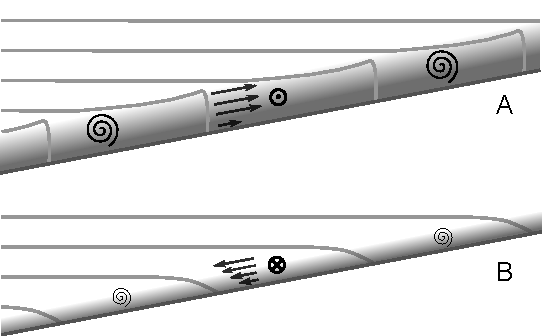
\includegraphics[width=30pc]{sketch.pdf}
  \caption{Slope-induced tidal straining causing (a) unstable
    stratification during upslope flow and (b) stable stratification
    during downslope flow (SIPS). Gray lines denote isopycnals, arrows
    show the current direction. Gray-shaded areas near the bottom
    indicate the presence of suspended material; spirals symbolize
    near-bottom turbulence.}
  \label{sketch}
\end{figure}

In a recent modeling study, \cite{schulzumlauf2016} proposed that
similar tidal straining and pumping processes may occur also in
vicinity of a topographic slope --- with the important difference,
however, that no externally imposed horizontal density gradient (e.g.,
due to river runoff) is required. In this case, the (quasi-)horizontal
density gradient is generated by the projection of the vertical
interior density gradient onto the slope
(Fig.\ \ref{sketch}). Slope-induced tidal straining is confined to a
turbulent bottom boundary layer (BBL), but the process is otherwise
completely analogous to classical tidal straining over a flat bottom:
during upslope flow, dense water is advected on top of lighter water,
resulting in unstable stratification, enhanced near-bottom turbulence,
and high concentrations of suspended material
(Fig.\ \ref{sketch}a). Vice-versa, during downslope flow, the
straining of the cross-slope density gradient induces a tendency for
increasing stratification inside the BBL, which in turn leads to
reduced BBL turbulence, smaller BBL thicknesses, and lower sediment
concentrations. Using an idealized one-dimensional (slope-normal)
numerical model, \cite{schulzumlauf2016} showed that tidal pumping
leads to a net cross-slope transport of suspended material, similar to
the tidal pumping mechanism over a flat bottom described by
\cite{JayMusiak94a}. In their study, \cite{schulzumlauf2016} ignored
the effect of rotation, which may, however, be essential in many
realistic settings. This point will therefore be investigated in
detail in the following analysis.

First observational evidence for slope-induced tidal straining was
recently discussed by \cite{Endohetal2016a}, who analyzed an extensive
data set, including turbulence microstructure observations, from a
topographic slope exposed to strong tidal currents in the East China
Sea. These authors described a periodic destabilization of the water
column during periods with upslope tidal currents, induced by the
presence of a persistent cross-slope density gradient. The latter
turned out to be consistent with the projection of the vertical
density gradient onto the slope, and therefore with the importance of
slope-induced tidal straining.

Here, we attempt to clarify the mechanisms, implications, and
relevance of slope-induced tidal straining on a real oceanic shelf by
combining the results from previous modeling studies by
\cite{UmlaufBurchard2011a} and \cite{schulzumlauf2016} with the
experimental data by \cite{Endohetal2016a}.  In section
\ref{modeldescription}, we extend the model used by
\cite{schulzumlauf2016} to include the effects of rotation before we
briefly summarize the field observations discussed by
\cite{Endohetal2016a} in section \ref{studysite}. After deriving model
parameters from these observations in section \ref{observations}, we
discuss the model results in section \ref{modelresults}, and compare
them to the field data. The implications of tidal straining for the
generation of residual currents and the residual transport of
suspended material are analyzed in section \ref{residualsjgr} before we
draw some conclusions in section \ref{conclusions}.


\section{Model description}\label{modeldescription}

\subsection{Model geometry}\label{modelgeometry}

Following previous modeling studies of slope-induced straining
\citep{UmlaufBurchard2011a,schulzumlauf2016}, we investigate in the
following the motion of a vertically stratified Boussinesq fluid in
the vicinity of a uniform slope with slope angle $\alpha$. The
geometry is two-dimensional with the horizontal and vertical
coordinates denoted by $\hat{x}$ and $\hat{z}$, respectively, and the
fluid is assumed to rotate with angular velocity $f / 2$ about the
vertical axes (Fig.\ \ref{geometry}). Vertical stratification is
quantified with the help of the buoyancy frequency,
\begin{equation}
  \label{N2}
  N^2 = \frac{\partial b}{\partial \hat{z}} \, ,
\end{equation}
where $b$ denotes buoyancy. Above the BBL, we assume that isopycnals
remain strictly horizontal during all times, and that $N^2$ approaches
the constant background value $N^2_\infty$. Close to the bottom,
however, isopycnals will be distorted as a result of boundary mixing,
and the local buoyancy $b$ will differ from the equilibrium buoyancy
$b_\infty$ (black and gray lines Fig.\ \ref{geometry}).

\begin{figure}
  \noindent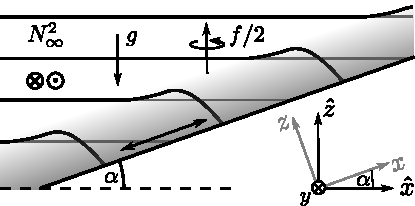
\includegraphics[width=30pc]{geometry.pdf}
  \caption{Schematic view of the model geometry and density structure
    (black lines) near a uniform slope with slope angle $\alpha$. Gray
    lines indicate isopycnal equilibrium levels ($b_\infty =
    const.$). Upslope and slope-normal coordinates are denoted by $x$
    and $z$, respectively. Arrows symbolize the oscillating
    near-bottom currents.}
  \label{geometry}
\end{figure}

Introducing a rotated coordinate system with the cross-slope,
along-slope, and slope-normal coordinates denoted by $x$, $y$, and $z$
(see Fig.\ \ref{geometry}), it can be shown from simple geometrical
arguments that under the above conditions also the cross-slope
buoyancy gradient is constant:
\begin{equation}
  \label{dbdxjgr}
  \frac{\partial b}{\partial x} = N^2_\infty \sin \alpha \, ,
\end{equation}
illustrating the generation of a quasi-horizontal ($\alpha \ll 1$)
buoyancy gradient by the projection of the purely vertical interior
stratification onto the slope
\citep{Garrettetal93a,UmlaufBurchard2011a}.

\subsection{Model equations}\label{modelequations}

Assuming that all cross-slope and along-slope gradients vanish, except
the cross-slope buoyancy gradient defined in (\ref{dbdxjgr}), the problem
becomes geometrically one-dimensional in the slope-normal
$z$-direction. The Boussinesq equations can then be written as
\citep{Umlaufetal2015a}:
\begin{align}
  \label{ueq}
  \frac{\partial u}{ \partial t} -fv \cos \alpha  &= (b - b_\infty) \sin \alpha 
+ P_x - \frac{\partial \tau_x}{ \partial z} \, , \\
  \label{veq}
  \frac{ \partial v}{\partial t} + fu \cos \alpha &= P_y - 
\frac{\partial \tau_y}{\partial z}                             \, , \\
  \label{beq}  
  \frac{\partial b}{\partial t} &= -u N^2_\infty \sin \alpha - 
\frac{\partial G}{\partial z}                              \, , 
\end{align}
with $u$ and $v$ denoting the upslope and along-slope velocities, and
$\tau_x$, $\tau_y$ and $G$ the slope-normal turbulent fluxes of
momentum (per unit mass) and buoyancy, respectively. $P_x(t)$ and
$P_y(t)$ are integration constants that play the role of prescribed
external pressure gradients. The cross-slope buoyancy gradient in the
advection term in (\ref{beq}) has been expressed with the help of
(\ref{dbdxjgr}). Note that in contrast to previous studies of
slope-induced tidal straining that only considered the plane
non-rotating case ($f=0$, $v=0$), equations (\ref{ueq}) -- (\ref {beq}) now
include rotational effects that turned out to be essential to describe
the motions at our study site.

The equilibrium buoyancy $b_\infty$ appearing in the first term on the
right hand side of (\ref{ueq}) evolves as a result of cross-slope
buoyancy advection, and can therefore be described by an advection
equation of the form.
\begin{equation}
  \label{binf}
  \frac{\partial b_\infty}{\partial t} + u_\infty N_\infty^2 \sin \alpha = 0 \, 
,
\end{equation}
which directly follows from (\ref{beq}) for $z \rightarrow \infty$.

Far away from the boundary ($z\rightarrow \infty$), we assume that all
slope-normal gradients, except the buoyancy gradient vanish, whereas at
the lower boundary ($z = 0$) we use the boundary conditions
\begin{equation}
  \label{uvbBC}
  u=v=0, \quad \frac{\partial b}{\partial z}=0 \, .
\end{equation}

\cite{schulzumlauf2016} also discussed a simple transport equation for
the concentration $c$ of suspended particulate material (SPM)
exhibiting a vertical sinking motion $w_s$ relative to the moving
fluid:
\begin{equation}
  \label{ceq}
  \frac{\partial c}{\partial t} = - \frac{\partial }{\partial z} \left( F_z - c 
w_s  \cos \alpha \right) \, , 
\end{equation}
where $F_z$ is the slope-normal turbulent SPM flux. At the bottom,
this flux equals the erosion flux:
\begin{equation}
  \label{Fzjgr}
  F_z = \alpha_e \max \left\{ \frac{|\tau_b|}{\tau_c} -1,0 \right\} \quad 
\text{at $z=0$} \, ,
\end{equation}
where $\alpha_e$ is the erosion parameter, $\tau_b$ the bottom stress,
and $\tau_c$ the critical shear stress for erosion.

The turbulent fluxes appearing in (\ref{ueq}) -- (\ref{beq}) and
(\ref{ceq}) are computed from gradient expressions of the form
\begin{equation}
  \label{turbfluxes}
  \tau_x = - \nu_t   \frac{\partial u}{\partial z} \, , \quad
  \tau_y = - \nu_t   \frac{\partial v}{\partial z} \, , \quad
  G      = - \nu^b_t \frac{\partial b}{\partial z} \, , \quad
  F_z    = - \nu^b_t \frac{\partial c}{\partial z} \, , 
\end{equation}
where $\nu_t$ is the turbulent viscosity, and $\nu^b_t$ the turbulent
diffusivity of buoyancy and SPM. The diffusivities are computed from a
second-moment turbulence model that includes two prognostic equations
for the turbulent kinetic energy $k$ and the dissipation rate
$\varepsilon$. This turbulence model is identical to that described in
detail in \cite{UmlaufBurchard2011a}, \cite{Umlaufetal2015a}, and
\cite{schulzumlauf2016}, and, for brevity, this description is not
repeated here. The general properties of this class of turbulence
models are reviewed in \cite{UmlaufBurchard2005a}; details about the
numerical implementation may be found in \cite{Umlaufetal2005a}. In
the non-turbulent region above the BBL ($z \rightarrow \infty$), the
turbulent fluxes are assumed to vanish.  Also, as we only investigate
flows at high Reynolds number in this study, all molecular fluxes are
ignored.

\subsection{Model properties}\label{modelproperties}
In the following, we will assume that BBL motions are driven by a
harmonic horizontal pressure force pointing into an arbitrary
horizontal direction, here referred to as the $n$-direction:
\begin{equation}
  \label{Pn}
  P_n = P \cos (\omega t + \phi) \; ,
\end{equation}
where $\omega$ is the forcing frequency, $\phi$ the phase, and $P$ the
magnitude of the pressure force. Denoting the angle between the $n$-
and $x$-directions as $\beta$, the components of $P_n$ in the $x$- and
$y$-directions are $P_x = P_n \cos \beta$ and $P_y = P_n \sin
\beta$. It is straightforward to show from (\ref{ueq}) and (\ref{veq})
that for the harmonic forcing in (\ref{Pn}), the velocities in the
inviscid region above the BBL ($z\rightarrow \infty$) are described by
\begin{align}
  \label{Un}
  u_n & = P \frac{\omega}{\omega^2 - f^2} \sin ( \omega t + \phi) \\
  u_s & = P \frac{f     }{\omega^2 - f^2} \cos ( \omega t + \phi) \, ,
  \label{Us}
\end{align}
with $u_n$ and $u_s$ denoting the components in the $n$- and
$s$-directions, respectively (the latter obtained from rotating the
$y$-axis by the angle $\beta$). For $\omega>f$, the velocity vector is
seen to anti-cyclonically trace an ellipse with axes ratio
$e=\omega/f$, where the main axis points into the direction of the
pressure gradient. Due to the lack of viscous damping in the
non-turbulent layer above the BBL, velocities increase toward infinity
if resonance is reached ($\omega=f$). The harmonic pressure term in
(\ref{Pn}) will be used below as a simple representation of tidal
forcing in a rotating system

The situation becomes more complex inside the BBL due to the
appearance of the internal pressure term $(b-b_\infty) \sin \alpha$ in
(\ref{ueq}). \cite{Umlaufetal2015a} showed that this term represents
the tendency of isopycnals to relax back to their equilibrium
positions ($b=b_\infty$), which implies the possibility of reversible
BBL oscillations at the frequency
\begin{equation}
  \label{omegacjgr}
  \omega_c^2 = f^2 \cos^2 \alpha + N_\infty^2 \sin^2 \alpha \, ,
\end{equation}
indicating that BBL resonance occurs for $\omega=\omega_c$
\citep{UmlaufBurchard2011a}. Vice-versa, if $N_\infty$, $f$, and
$\omega$ are considered to be given, BBL resonance will be observed if
the slope $\alpha$ approaches the critical slope $\alpha_c$ found from
inverting (\ref{omegacjgr}). Model properties exhibit qualitative changes
during the transition from subcritical to supercritical slopes, and
some of the model assumptions break down near critical slopes
\citep{UmlaufBurchard2011a,schulzumlauf2016}.

Near the geographic location investigated in this study, the
parameters $N^2_\infty,\, f,$ and $\alpha$ are derived in the chapters
below and summarized in Tab.\ \ref{input}. The frequency for critical
boundary layer resonance derived from these parameters is $\omega_c =
7.69 \times 10^{-5}$~s~$^{-1}$, corresponding to a period of $T_c = 22.7$~h. As
discussed in more detail below, the proximity of $T_c$ to the diurnal
tidal period is one of the reason why the diurnal tides are neglected
in our model analysis.

\begin{table}
\caption{Standard parameters used for the simulations in sections
  \ref{modelresults} and \ref{residualsjgr}}\label{input}
\begin{center}
\begin{tabular}{ccccccc}
\hline
\hline
$\alpha$ & $N_\infty^2$ & $f$ & $z_0$ & $\tau_c$ & $\alpha_e$ \\
\hline
$3 \times 10^{-4}$ & $6.5 \times 10^{-4}\, \text{s}^{-2}$ & $7.65 \times 
10^{-5}\, 
\text{s}^{-1}$ & $10^{-3}\, \text{m}$ & $10^{-4}$~m$^2$~s$^{-2}$ & 
$10^{-4}$~kg~s$^{-1}$~m$^{-2}$ \\
\hline
\end{tabular}
\end{center}
\end{table}

Finally, for the following discussion of residual transports it is
useful to note that \cite{UmlaufBurchard2011a} showed that under the
above conditions (harmonic forcing, zero mixing above the BBL), the
residual upslope transport vanishes
\begin{equation}
  \label{uint}
  \int_0^\infty \langle u \rangle dz = 0 \, ,
\end{equation}
where the angular brackets denote the average over one forcing period
$T = 2 \pi / \omega$.

\section{Study site and methods}\label{methods}

\subsection{Study site}

In July 2011, hydrographic and turbulence microstructure measurements
were performed near position S in the East China Sea
(Fig.\ \ref{studysite}). The study site was located at $31^\circ
44.9'\,\text{N}, \, 125^\circ 50.0'\,\text{E}$ on a mildly sloping
continental shelf at approximately 68~m water depth. The inertial
period at this latitude is $T_f = 23.3$ hours. Based on a
finite-element global ocean tidal model with a regionally refined
numerical grid, \cite{Lefevreetal2000} showed that the East China Sea
is subject of strong tidal motions with the four major constituents
being: the principal lunar and solar tides, $M_2$ and $S_2$, with
semi-diurnal periods, and the luni-solar and principal lunar diurnal
tides, $K_1$ and $O_1$, respectively. The $M_2$ tide is dominant here,
about three times stronger than the second largest tidal component,
the $S_2$. The two diurnal tides are of similar magnitude and about 4
times weaker than the $M_2$ component. Similar results were derived from 
observations of current velocity data at  $31^\circ 45'\,\text{N}, \, 127^\circ 
25'\,\text{E}$ (east of position S) \citep[][]{Yoshikawaetal2012a}. It should 
be noted that the inertial period is close to the periods of the diurnal tides,
precluding a straightforward spectral distinction between diurnal
tidal and near-inertial signals in a short time series.

\begin{figure}
  \noindent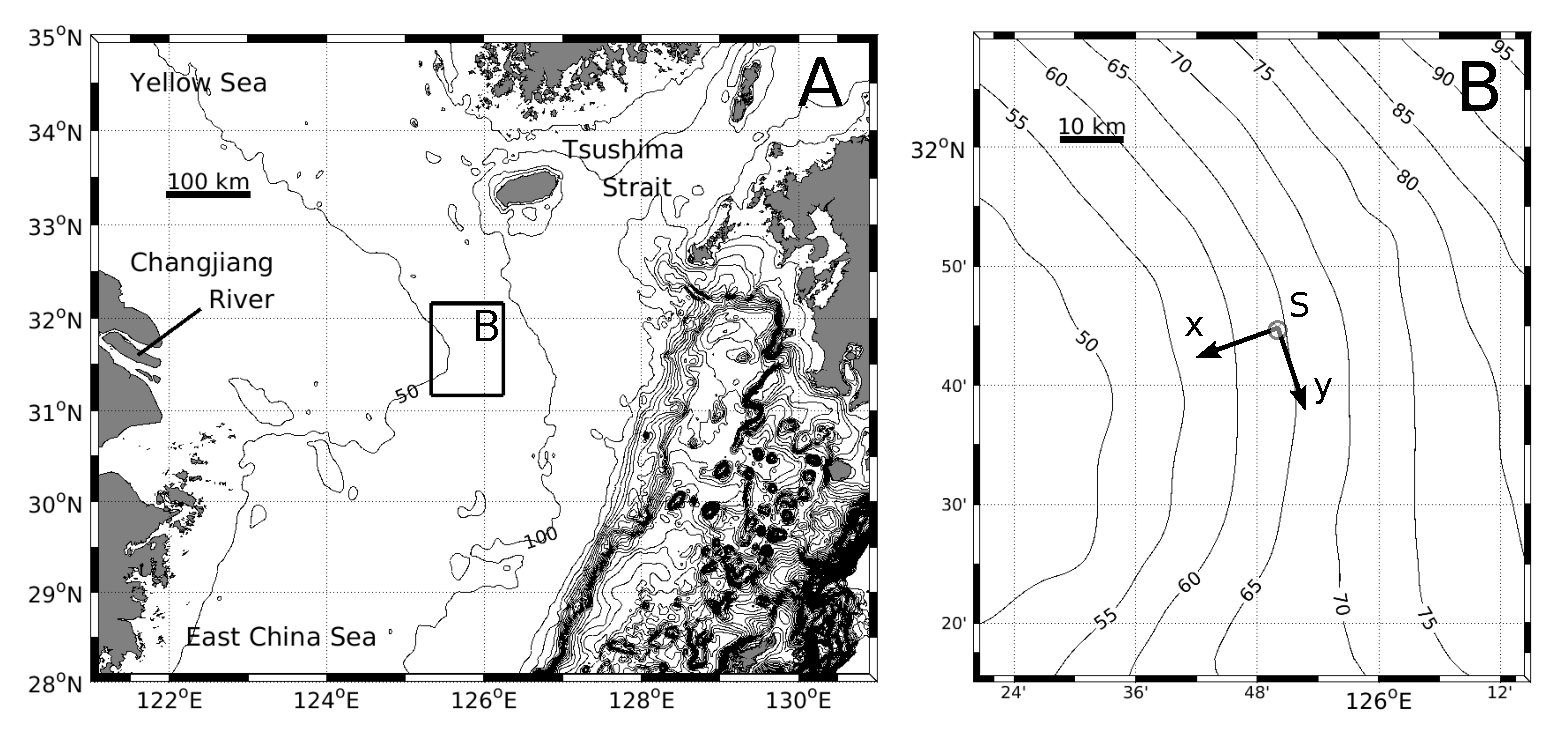
\includegraphics[width=35pc]{studyside.pdf}
  \caption{Maps of (a) East China Sea, and (b) study area with
    deployment location ``S''. Local cross-slope and along-slope
    directions are denoted by $x$ and $y$ (rotated by 20 degrees with
    respect to the zonal and meridional directions,
    respectively). Bathymetry is in meters, based on bathymetric data
    described in \cite{Choietal2002a}.}
  \label{studysite}
\end{figure}

Fig.\ \ref{studysite} illustrates that position S is located
approximately 400~km away from the Changjiang river mouth, which forms
the by far largest freshwater source in this
region. \cite{Endohetal2016a} pointed out that this large spatial
separation, and the fact that the less dense river water will mainly
affect the near-surface layer during the thermally stratified summer
period, suggests that the BBL at position S is unlikely to be
dynamically influenced by freshwater runoff.

In the area of interest, the main axis of the bottom slope, i.e.\ the
direction of maximum inclination, is orientated approximately $20$
degrees relative to the zonal direction (Fig.\ \ref{studysite}b). To
be consistent with the model geometry shown in Fig.\ \ref{geometry},
we introduce a local coordinate system with the $x$- and $y$-axes
pointing in the upslope and along-slope directions, respectively, as
indicated in Fig.\ \ref{studysite}b. Using an identical coordinate
system, \cite{Endohetal2016a} showed that the along-slope density
gradient is nearly negligible compared to the cross-slope
gradient. They also found that the observed periodic density
variations in the BBL were largely caused the by up- and downslope
advection of isopycnals due to the tides, which forms the most
important prerequisite for the occurrence of slope-induced tidal
straining (see Fig.\ \ref{sketch}).

Echosounding data from the cruise (not shown) showed that the
bathymetry exhibits a nearly perfectly linear slope in the
$x$-direction on horizontal scales of the order of a few tens of
kilometers. According to these data, the topographic slope is
approximately $3 \times 10^ {-4}$, which is also taken as the default
value for the numerical simulations described below. Several
bathymetric data sets for the East China Sea are available, but due to
their coarse resolution the slope angle near position S tends to be
somewhat overestimated. Recent topographic data discussed in
\cite{Choietal2002a} suggests, e.g., a slope of nearly $6 \times
10^{-4}$ near the study site. The sensitivity of our results with
respect to these uncertainties in the slope angle will be discussed
in Appendix B.

\subsection{Methods}

The dataset we discuss here was collected with a 600-kHz ADCP
(Workhorse from Teledyne RD Instruments) and a tethered turbulence
microstructure profiler (TurboMAP-5 from JFE Advantech, Japan) during
a cruise of the training ship Nagasaki-Maru in July 2011. Echo
sounding data were obtained with a KFC-300 quantitative echo sounder
from Sonic, Japan.

The ADCP was mounted on a trawl-resistant bottom frame, and deployed
on the seabed from 16:40 JST (Japan Standard Time) on 16 July to 15:40
JST on 21 July. The vertical bin size was set to 1~m, and the depth of
the first bin was located 3~m above the seabed, i.e.\ at approximately
65 m depth. The ADCP was operated in standard RDI ``mode 1'', sampling
the along-beam velocities at a rate of 1.3~Hz during 20-minute bursts
starting every half hour. From the along-beam velocities averaged over
20 minutes (1600 pings), the horizontal components of the velocity were 
calculated at half-hour intervals.

The microstructure profiler was deployed from the ship within about
500~m distance from the ADCP between 17:00 JST on 17 July and 06:00
JST on 19 July. While the profiler was freely descending at a speed of
0.5 -- 0.6~m~s$^{-1}$, vertical shear and temperature microstructure
were sampled at a rate of 512~Hz, whereas temperature, conductivity,
pressure, turbidity, fluorescence, and the acceleration of the
instrument were sampled at a rate of 64~Hz. A total of 101 profiles
between a depth of 10 m and the bottom were obtained. From the
microscale vertical shear, the dissipation rate of turbulent kinetic
energy, $\varepsilon$, was estimated, assuming locally isotropic
turbulence \citep[][]{Hinze1987} across 1-m windows as described in
more detail in \cite{Endohetal2016a}. A series of 1-3 profiles taken
approximately every hour was averaged to provide hourly means.

\subsection{Analysis of tidal motions}

Tidal forcing parameters for the idealized simulations described below
were found by extracting the major tidal constituents from the
velocities observed at position S. We performed this tidal analysis
based on the velocity records at 30~m depth (38~m above the bottom),
noting that results were not particularly sensitive with respect to
small variations of this parameter. This choice for the ADCP reference
level was found to be a reasonable compromise between data quality
(deteriorating with increasing distance from the ADCP) and our attempt
to reduce the impact of bottom friction (increasing towards the
bottom). Prior to the following analysis, the velocities were
projected onto the topography-following $x$- and $y$-directions shown
in Fig.\ \ref{studysite}b.

\begin{figure}
  \noindent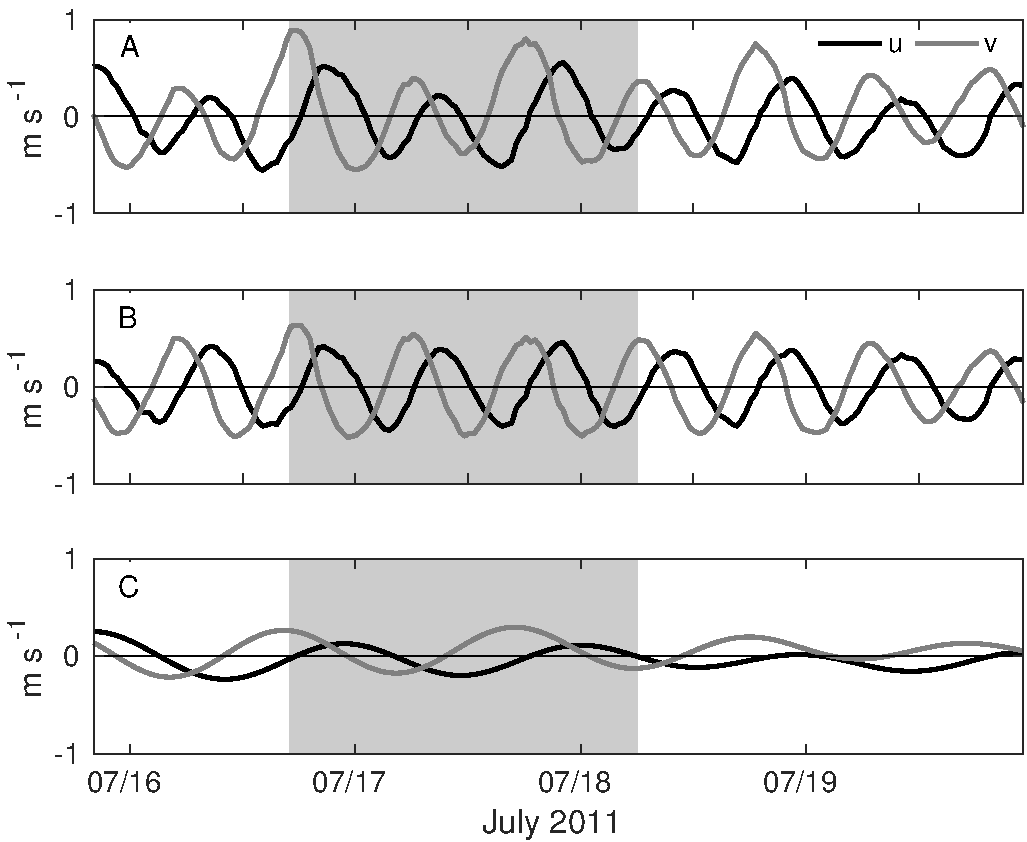
\includegraphics[width=30pc]{timeseries.pdf}
  \caption{Time-series of cross-slope ($u$) and along-slope ($v$)
    velocity components based on ADCP measurements in 30~m depth at
    position S: (a) unfiltered data, (b) highpass-filtered $M_2$ tidal
    currents, and (c) lowpass-filtered diurnal
    and subtidal currents. Period with microstructure measurements at
    position S is indicated in gray.}
  \label{tides}
\end{figure}

To decompose the observed signals into semi-diurnal and diurnal
components, we used a phase-preserving high-order filter with a cutoff
frequency of 15 hours. Comparison of the unfiltered
(Fig.\ \ref{tides}a) and highpass-filtered semi-diurnal velocities
(Fig.\ \ref{tides}b) clearly shows that the currents at our study site
were dominated by a regular $M_2$ tide with an amplitude of
approximately 0.5 m~s$^{-1}$, with slightly more energy in the
along-slope direction. This tidal constituent explains approximately
83\% of the total variance of the signal. The diurnal signal
(Fig.\ \ref{tides}c) is substantially weaker, and shows a clear trend
for both decreasing magnitude and and increasing frequency during the
observational period. Pure tidal motions are unlikely to exhibit such
variability on a time scale of only a few days, suggesting that the
observed signal is a mixture of near-inertial motions, which may
quickly vary in time due to their direct dependence on the wind
forcing, and different diurnal tidal constituents.

It is worth noting that a detailed tidal model of the East China Sea
by \cite{Baoetal2000} yields a velocity amplitude of approximately
0.5~m~s$^{-1}$ for the $M_2$ component at position S, in good
agreement with our data. For the diurnal $K_1$ tide, velocity amplitudes around
0.1~m~s$^{-1}$ were found, approximately twice as large as those of the
$O_1$ constituent. Our observations (see Fig.\ \ref{tides}c) suggest
that the model of \cite{Baoetal2000} slightly overestimates tidal
motions in the diurnal frequency band.

\section{Observations and model parameters}\label{observations}

\subsection{Observations}

The observations at position S have been described in detail by
\cite{Endohetal2016a}. Here, we only summarize their main findings to
provide the context for the discussion of the models results below.

Fig.\ \ref{meanprofiles} shows the averaged vertical structure of
salinity $S$, potential temperature $\theta$, potential buoyancy $b$,
and the (square of the) buoyancy frequency $N^2$, based on the average
of all profiles obtained at position S. Here, we define the buoyancy
as $b = - g (\rho_\theta-\rho_0)/\rho_0$, where $\rho_\theta$ is
potential density and $\rho_0=1000$~kg~m$^{-3}$ a constant reference
density. The figure shows that the lower part of the water column is
characterized by a nearly well-mixed BBL of more than 35~m thickness,
capped by a strongly stratified ``interior'' region with approximately
linear stratification, slightly larger than $N^2=10^{-3}$~s$^{-2}$.
Inside the BBL, the average stratification is 1-2 orders of magnitude
smaller compared to this interior region (Fig.\ \ref{meanprofiles}d).

\begin{figure}[ht]
  \noindent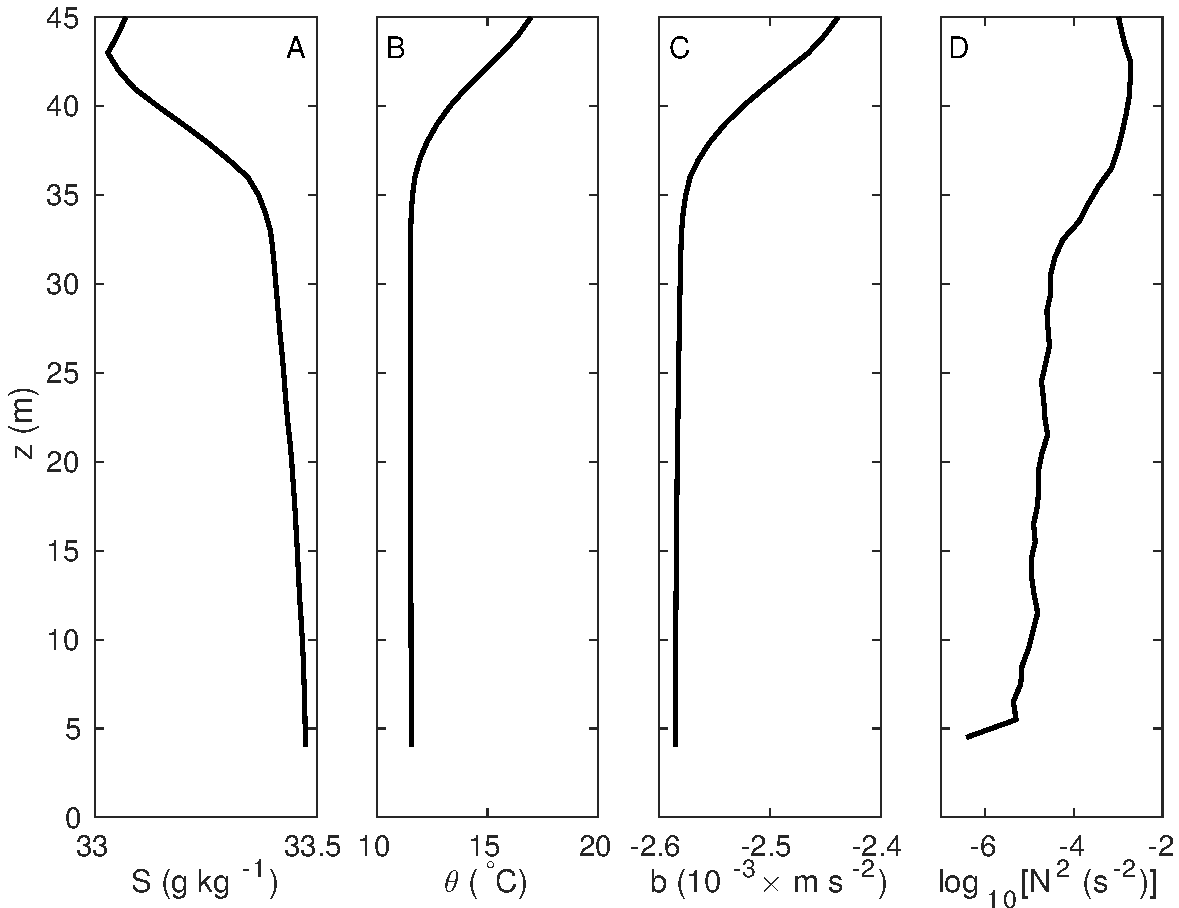
\includegraphics[width=30pc]{res_daten.pdf}
  \caption{Mean profiles of: (a) salinity, (b) potential temperature,
    (c) buoyancy, and (d) buoyancy frequency squared. Profiles are based on the 
average of all available microstructure profiles at station S (gray-shaded 
period in Fig.\ \ref{tides}).}
  \label{meanprofiles}
\end{figure}

As already discussed in the context of Fig.\ \ref{tides}, BBL
velocities are dominated by regular $M_2$ tidal motions, however, with
a significant diurnal modulation and indications for a frictional
reduction of the tidal velocities toward the bottom
(Fig.\ \ref{fielddata}a,b). Also the buoyancy anomaly
$\tilde{b}=b-\langle b \rangle$, where $ \langle b \rangle$ denotes
the tidally-averaged buoyancy shown in Fig.\ \ref{meanprofiles}c, is
characterized by a clear $M_2$ tidal variability with a $\pi/2$ phase
lag with respect to the $u$-component (Fig.\ \ref{fielddata}c). This
phase shift is expected if buoyancy variations are due to advection of
a constant cross-slope buoyancy gradient as mathematically described
by (\ref{beq}).

\begin{figure}[ht]
  \noindent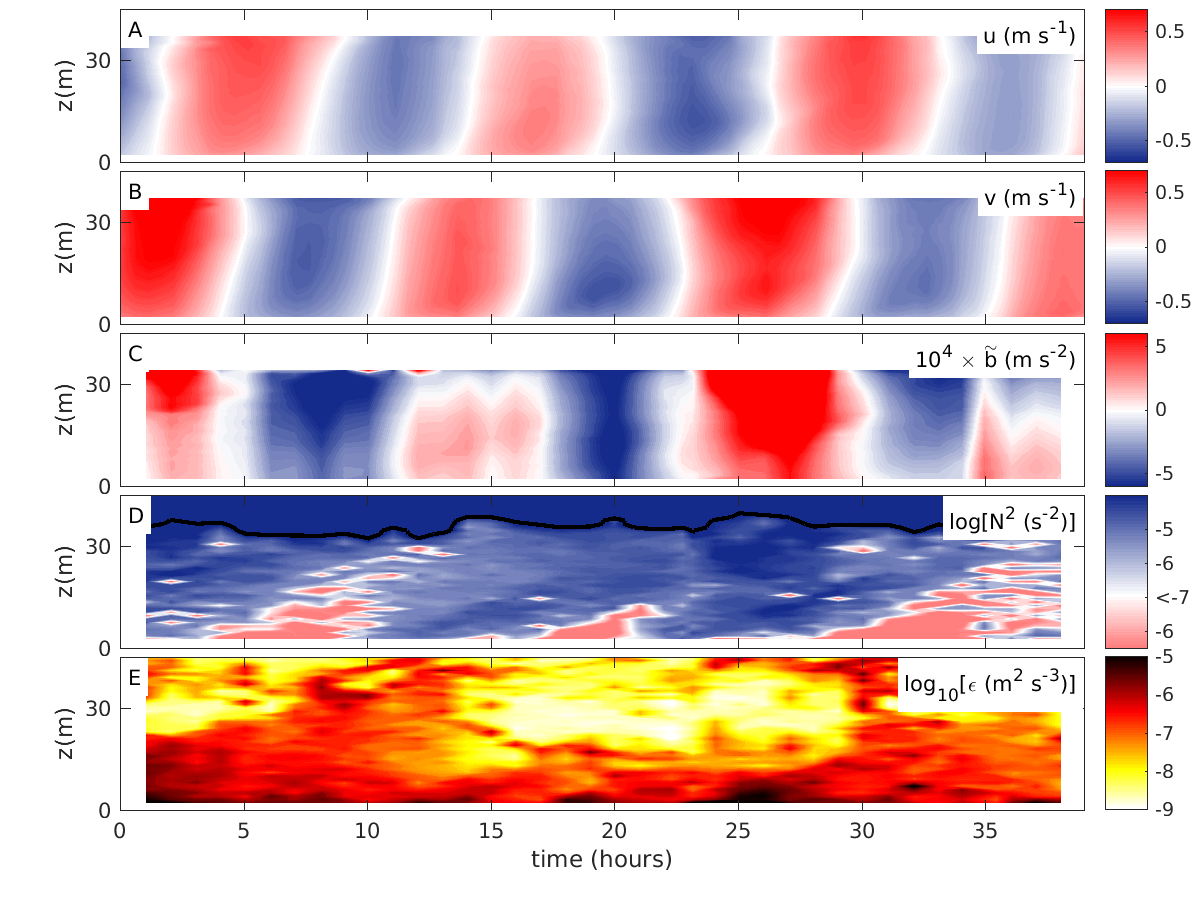
\includegraphics[width=40pc]{daten_teos10.png}
  \caption{Evolution of observed (a) cross-slope velocity, (b)
    along-slope velocity, (c) buoyancy fluctuations, (d) buoyancy
    frequency, and (e) turbulence dissipation rate. Note the special
    logarithmic color scale in (d): for $N^2 < 0$ (unstable
    stratification), the value of $| N^2 |$ is plotted in red shading,
    whereas regions with positive $N^2$ are plotted in blue
    shading. The black line indicates values of $N^2 = 10^{-3.7}$~s$^{-2}$ and 
    marks the vertical extent of the BBL. The time axis starts on 17 July 
    16:00 JST.}
  \label{fielddata}
\end{figure}

In the context of the present study, the most interesting feature in
these observations is the periodic destabilization of the lower part
of the BBL (Fig.\ \ref{fielddata}d) that \cite{Endohetal2016a} showed
to be consistent with slope-induced tidal straining as delineated in
Fig.\ \ref{sketch}. These unstable regions appear at the $M_2$ tidal
frequency, exhibit a significant vertical phase shift, and affect a
large fraction of the BBL. Beyond the key role played by the $M_2$
tidal currents in this processes a diurnal suppression of the vertical extent 
of 
the unstable regions is visible in Fig.\ \ref{fielddata}c), which should be 
kept in mind when interpreting the model results below (the diurnal signal is 
neglected in our model forcing).

Despite the dominant $M_2$ tidal forcing, the turbulence dissipation
rates shown in Fig.\ \ref{fielddata}d do not exhibit a clear tidal
signal. This is easily understood from the fact that the near-bottom
velocity vector at position S essentially rotates at the $M_2$ tidal
frequency without large modulations in magnitude (Fig.\ \ref{tides}c),
different from previous field studies in regions with more rectilinear
tides \citep[e.g.][]{Simpsonetal2002,Burchardetal2002a}. Noticeable is 
therefore 
in particular a diurnal modulation of the dissipation rate that is shown to be 
related to the vertical shear caused by the interference between diurnal and 
semidiurnal tidal currents rather than to the lateral advection of 
stratification in the upper part of the BBL \citep{Wakataetal2016a}.


\subsection{Model parameters}\label{parameters}

The solution of the system of equations in (\ref{ueq}) - (\ref{uvbBC})
depends on a number of model parameters that determine: the properties
of the rotating fluid ($f$, $N_\infty$), the slope ($\alpha$, $z_0$),
and the tidal forcing ($P_x$, $P_y$). In addition, if the transport of
suspended material is considered, the erosion parameter $\alpha_e$,
the critical shear-stress $\tau_c$, and the sinking speed $w_s$
appearing (\ref{ceq}) and (\ref{Fzjgr}) have to be specified.

Most obvious is the choice of the Coriolis parameter ($f=7.65 \times
10^{-5}$~s$^{-1}$) and the bottom slope ($\alpha=3 \times 10^{-4}$),
which can be determined without further assumptions from the local
latitude and the echo sounding data obtained during the cruise,
respectively (see above). As the bottom roughness is not well
constrained, we chose a standard value here ($z_0=0.001$~m), and
discuss the sensitivity of our results with respect to this parameter
in Appendix B.

The determination of the time-dependent forcing functions $P_x(t)$ and
$P_y(t)$ is based on the following considerations. Firstly, we require
a purely monochromatic forcing as in (\ref{Pn}) in order to allow the
model to reach periodic conditions after an appropriate spin-up period
to be able to compute well-defined tidal averages. Secondly, in view
of the idealized nature of our model, we will focus on forcing
functions that are as simple as possible but still sufficient to
mirror all key features of the observed BBL dynamics.

With this rationale in mind, and recalling that the $M_2$ tide largely
determines the observed velocity variance at our study site, we
computed the forcing functions based on the amplitude and phase of a
pure $M_2$ tide with period $T_{M_2} = 12.42\,\text{h}$. Also, as
discussed above in the context of (\ref{omegacjgr}), the diurnal tidal
components are close to the critical period, $T_c=22.7$~h, which is
likely to induce unphysical resonance effects in the modeled BBL.

We thus fitted a sinusoidal $M_2$ signal to the highpass-filtered
velocity data shown in Fig.\ \ref{tides}b, using the standard
least-squares fitting procedure described in \cite{EmeryThomson2001a},
however, with the following difference: the axes ratio of the tidal
ellipse was kept fixed at the value $\omega/f$ for consistency with
the model solution in (\ref{Un}). This modified fitting procedure
yields a tidal ellipse with a velocity amplitude of 0.53~m~s$^{-1}$
along the major axis, which is rotated at an angle of 107 degrees
counter-clockwise with respect to the along slope direction (see
Fig.\ \ref{fitellipse}). The analytical solution is seen to slightly
overestimate the observed ellipticity but provides otherwise a good
representation of the data.  It is worth noting that orientation and
tidal amplitude are also consistent with the $M_2$ tidal ellipse found
by \cite{Baoetal2000} near this position.

\begin{figure}
  \noindent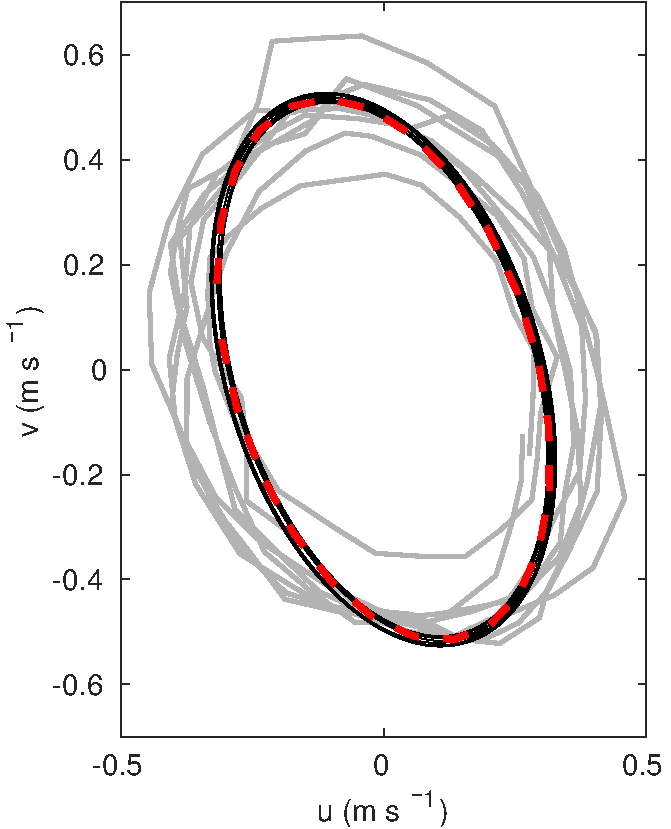
\includegraphics[width=20pc]{fitellipse.pdf}
  \caption{Highpass-filtered $M_2$ tidal currents at 30~m depth (light
    gray) and modeled velocities in the region above the BBL (black
    lines). The dashed red line indicates a fit to the data based on a
    tidal ellipse with prescribed axes ratio $\omega \slash f$.}
  \label{fitellipse}
\end{figure}

In the next step, we computed amplitude and phase of the pressure
function $P_n$ defined in (\ref{Pn}) be inverting (\ref{Un}), using
the observed velocity amplitude. Projecting the result onto the $x$-
and $y$-directions finally yields the required pressure functions
$P_x(t)$ and $P_y(t)$. As shown above, fully periodic model solutions
for this type of pressure forcing correspond to the tidal ellipse
described by (\ref{Un}) in the non-turbulent model region above the
BBL. However, numerical tests have shown that transients (mainly
inertial oscillations) generated during the abrupt start of the
simulations do not decay in this region due to the lack of any
physical damping mechanism. The problem can be strongly reduced (but
not fully eliminated) by linearly increasing the periodic pressure
forcing from zero to full amplitude over a period of 10 days. After a
spin-up period of additional 40 days, the solutions become fully
periodic inside the BBL (where transients quickly decay as a result of
viscous damping) and nearly periodic in the undamped region above the
BBL (see Fig.\ \ref{fitellipse}). As we are only interested in the
processes inside the BBL, small deviations from perfect periodicity
above the BBL are of no consequence for the following analyses.

Finally, the relevant background stratification $N_\infty$ can be
conveniently computed from the cross-slope buoyancy gradient $\partial
b / \partial x$, using the projection relation in (\ref{dbdxjgr}). Here,
we estimate $\partial b / \partial x$ following \cite{Endohetal2016a},
who noted that buoyancy fluctuations inside the nearly well-mixed BBL
are largely determined by up- and downslope advection. Thus, for this
purpose, the buoyancy equation in (\ref{beq}) can be approximated as
\begin{equation}
  \label{badv}
  \frac{\partial b}{\partial t} = -u \frac{\partial b}{\partial x} \; ,
\end{equation}
assuming that $\partial b / \partial x$ is constant.

Similar to \cite{Endohetal2016a}, we find that $\partial b / \partial
x=2 \times 10^{-7}$~s$^{-2}$ largely explains the observed buoyancy
fluctuations due cross-slope tidal motions (see below). According to
(\ref{dbdxjgr}), for the observed bottom slope, this value yields
$N_\infty^2 \approx 7 \times 10^{-4}$~s$^{-2}$, slightly smaller than
the measured vertical stratification above the BBL
(Fig.\ \ref{meanprofiles}d) but of the correct order of magnitude. As
pointed out by \cite{Endohetal2016a}, the relevant interior
stratification for slope-induced tidal straining is that
\emph{adjacent} to the BBL (i.e., in the interior region located at
the same depth level as the BBL at position S) rather than
\emph{above} the BBL. It is likely that the real interior
stratification adjacent to the BBL, rather than being vertically
homogeneous as assumed in our model, slightly decays with depth away
from the thermocline region.

\section{Modeling slope-induced tidal straining} \label{modelresults}

Using the periodic tidal forcing described in
section~\ref{modelproperties}, and the model parameters in
Tab.\ref{input}, we investigate in the following to which extent our
idealized model is able to reproduce the features of the observed
BBLs. For easier comparison between field data (Fig.\ \ref{fielddata})
and model results (Fig.\ \ref{modeloutcome}), time axes have been
aligned to reproduce the correct phase relationships in the $M_2$
tidal currents after the model has become periodically stationary. Due
to their periodic nature, model results are only shown for two tidal
periods for clarity.

\begin{figure}
  \noindent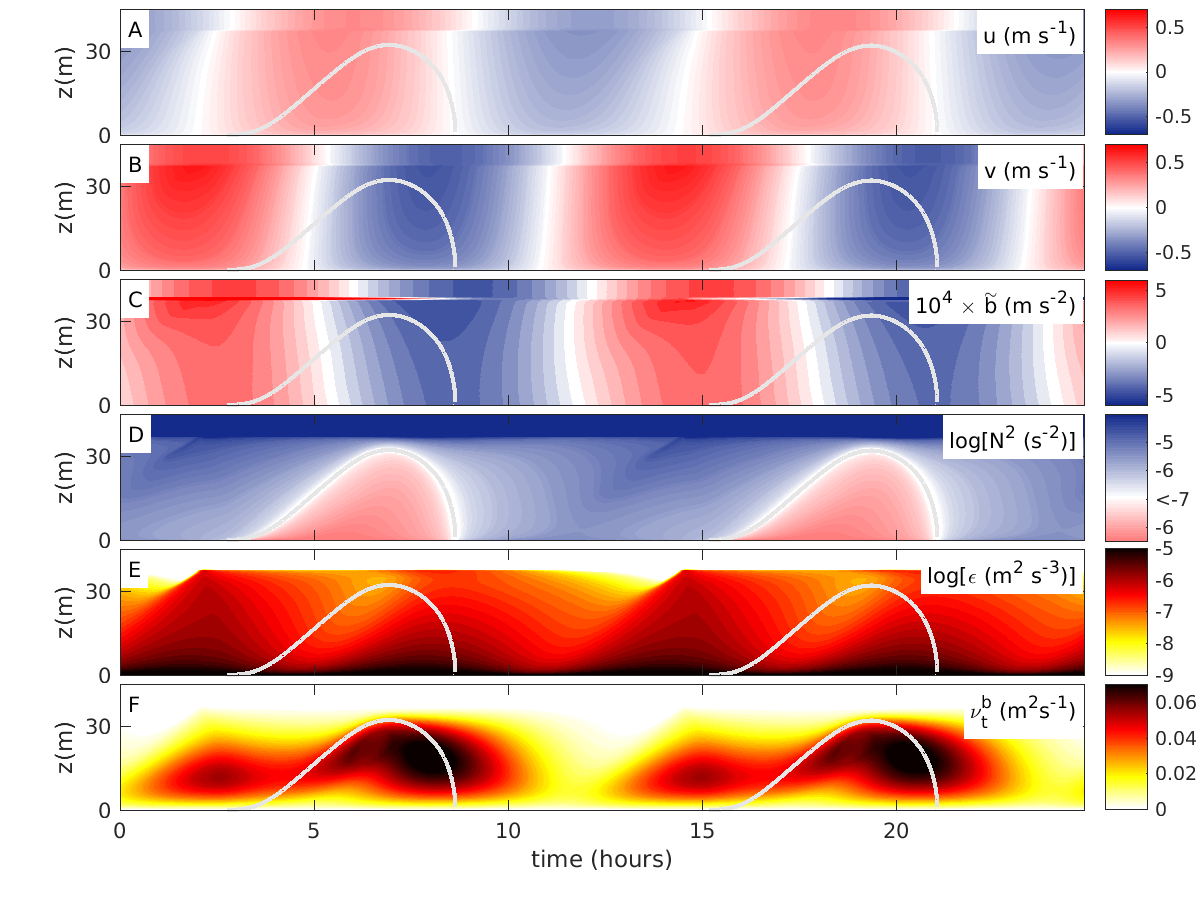
\includegraphics[width=40pc]{modeloutcome.png}
  \caption{Evolution of modeled (a) cross-slope velocity, (b)
    along-slope velocity, (c) buoyancy fluctuations, (d) buoyancy
    frequency, (e) turbulence dissipation rate, and (f) turbulent
    diffusivity. Gravitationally unstable regions are indicated by
    gray lines in all panels. Axes ranges, color scales, and time axis
    are identical to those used in Fig.\ \ref{fielddata}. }
  \label{modeloutcome}
\end{figure}

The modeled velocities (Fig.\ \ref{modeloutcome}a,b) mirror the
observed $M_2$ tidal variability with good accuracy but do not exhibit
the observed diurnal modulation, which is obviously a consequence of
neglecting the diurnal tidal constituents in our simulations. As
explained above, the diurnal signal is significant but not essential
for the process studied here.  Similar to the observations, also the
model results show clear indications for a frictional reduction of the
velocities towards the bottom, which is an essential requirement for
the development of SIPS.

Also the magnitude and phase of the tidal buoyancy fluctuations shown
in Fig.\ \ref{modeloutcome}c are in good agreement with the data,
supporting the idea that the variability in buoyancy is largely a
result of cross-slope advection as discussed above. The strong diurnal
modulation of the buoyancy fluctuations in the upper part of the BBL
found in the observations is, however, not represented by the
model, as diurnal tides are ignored in our simulations.

While the good agreement between model and data regarding the tidal
velocity and buoyancy fluctuations is largely a result of the selected
forcing variables and model parameters, the correct prediction of BBL
stratification provides a much more stringent test of the model
performance. Fig.\ \ref{modeloutcome}d shows that the model provides
an excellent representation of the evolution of BBL stratification in
at least two important aspects. First, the predicted BBL thickness is
approximately 37~m, and therefore well inside the observational range
(see Fig.\ \ref{fielddata}d). In view of the complex interplay between
slope-induced re-stratification and mixing that determines the BBL
thickness, this is a remarkable result. Second, the model is also able
to reproduce the periodic generation and destruction of stratification
(SIPS) inside the BBL, in particular regarding the occurrence of
gravitationally unstable layers during periods of upslope flow. The
observed and modeled unstable layers have a similar vertical extent
and timing but, different from the model, the observations also
exhibit a strong diurnal modulation of stratification that leads to a
suppression of the convective layer thickness during every second
instance of their occurrence (e.g., at $t \approx 20$~h in
Fig.\ \ref{fielddata}d), which cannot be reproduced in the model, of course,
again because diurnal tides are ignored.

As pointed out above, the imprint of this diurnal modulation in
stratification is also clearly visible in the observed dissipation
rates (Fig.\ \ref{fielddata}e) but, for the reasons described above,
cannot be reproduced by the model. The model does, however, correctly
predict the strong increase of the dissipation rates towards the
bottom, and the correct order of magnitude of dissipation at the
beginning and end of observation period (Fig.\ \ref{modeloutcome}e). Modeled
dissipation rates show a $M_4$ periodicity with a $M_2$ modulation
that reflects the ellipticy of the tidal currents: largest dissipation
rates are found at peaks of the $v$-component, which dominates the
$M_2$ tidal motions (see above).

While the variability in the modeled dissipation rates is therefore
mainly driven by variations in tidal forcing, the eddy diffusivities
shown in Fig.\ \ref{modeloutcome}f are also strong affected by
variations in stratification associated with SIPS. Although peaks in
dissipation rate and eddy diffusivity approximately coincide, the
latter shows a much stronger tidal asymmetry: largest diffusivities
are found during periods of upslope flow, when slope-induced tidal
straining reduces vertical stratification, or even causes regions with
negative $N^2$. We will see in the following that this modulation of
the eddy diffusivity is essential for the generation of residual
transports.



\section{Dynamics of suspended material} \label{residualsjgr}

One of the most important implications of tidal straining is the
generation of residual currents and residual transports of dissolved
substances and suspended material. \cite{Endohetal2016a} speculated
that this process may also play an essential role for the transport of
suspended material at their study site in the East China Sea. Although
their turbidity measurements (see their Fig.\ 2i) clearly show
strongly enhanced concentrations of suspended material inside the BBL,
their data were too limited to draw any definite conclusions about
residual SPM transports. In the following, we therefore discuss a
number of idealized simulations to clarify the mechanisms and
potential implications of slope-induced tidal straining for the
residual transport of suspended material.

\subsection{Temporal variability}\label{temporal}

Our simulations are based on the SPM transport equation in (\ref{ceq})
and the simple erosion model in (\ref{Fzjgr}). Lacking information about
sediment properties at the study site, we vary the sinking speed,
identified by \cite{schulzumlauf2016} as the key parameter
determining the transport of suspended material, over a broad range of
values. For the critical shear stress, $\tau_c$, and the erosion
parameter, $\alpha_e$, shown to be of only secondary importance by
\cite{schulzumlauf2016}, we adopt the standard values suggested by
these authors (see Tab.\ \ref{input}).

\begin{figure}[ht]
  \noindent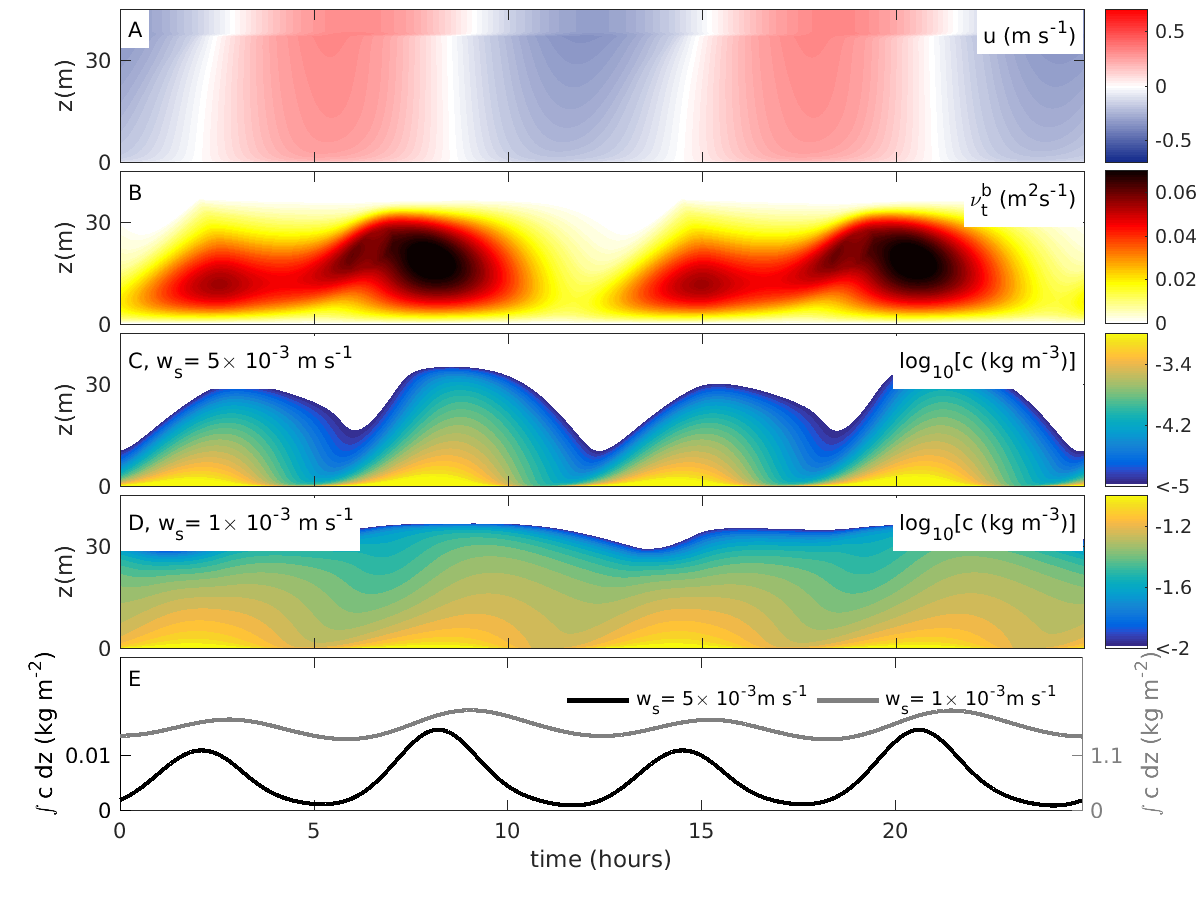
\includegraphics[width=40pc]{divc.png}
  \caption{Evolution of (a) cross-slope velocity, (b) turbulent
    diffusivity, and (c,d) SPM concentrations for two different
    settling velocities: $w_s=5 \times 10^{-3}$~m~s$^{-1}$ and $w_s=1
    \times 10^{-3}$~m~s$^{-1}$. Panel (e) shows the corresponding
    integrated SPM concentrations. Panels (a) and (b) are re-drawn
    from Fig.\ \ref{modeloutcome}a,f for better orientation.}
  \label{wsdifference}
\end{figure}

Fig.\ \ref{wsdifference}c,d reveals for two different sinking speeds
that maxima in the SPM concentrations follow maxima in the turbulence
diffusivities with a small phase shift, which mirrors the time
required to mix eroded material up into the BBL. Concentration maxima
are found when the cross-slope velocity $u$ is close to zero
(Fig.\ \ref{wsdifference}a), or, likewise, when the magnitude of the
more energetic along-slope flow component $v$ attains maximum values
(Fig.\ \ref{modeloutcome}b). Tidal asymmetries resulting from the
modulation of the turbulent diffusivity due to SIPS are clearly
evident in both local and vertically integrated SPM concentrations
(Fig.\ \ref{wsdifference}c-e). For large sinking speeds
(Fig.\ \ref{wsdifference}c), highest concentrations are found at the
end of the period with upslope flow, when turbulent diffusivities are
maximum, along-slope velocities close to their maximum negative values
($v<0$), and cross-slope velocities close to zero. Similar SPM maxima
are also found at the end of downslope flow period, however, with
significantly smaller concentrations due to the comparably smaller
turbulent diffusivities.

The strong correlation between high SPM concentrations and negative
along-slope speeds constitutes a tidal pumping mechanism that, as
discussed in more detail below, leads to a vigorous residual transport
of suspended material along the slope in the negative
$y$-direction. Tidal pumping is much less effective in the cross-slope
$x$-direction because SPM concentration maxima are associated with
minima in the magnitude of the cross-slope velocity ($u \approx
0$). Although tidal asymmetries in SPM concentrations can also be
discerned for the case with low sinking speeds
(Fig.\ \ref{wsdifference}d,e), they are less pronounced, and their
potential to trigger tidal pumping is therefore expected to weaker.

Finally, it is worth noting that the collapse of cross-slope tidal
pumping mentioned above is qualitatively different from the
non-rotating case investigated by \cite{schulzumlauf2016}. Although
their simulations showed similar tidal asymmetries with highest
turbulent diffusivities and SPM concentrations observed during periods
of upslope flow, these maxima occurred earlier compared to the rotating
case. This is easily understood from the fact that in the non-rotating
case the $v$-component, dominating BBL turbulence in our case, is
lacking, and highest diffusivities are thus observed significantly
before the upslope flow reversal. In the non-rotating case, high SPM
concentrations are therefore correlated with significant upslope
velocities ($u>0$), resulting in an effective upslope pumping of
suspended material.


\subsection{Residual transports}\label{residualtransports}
The residual transports of suspended material in the cross-slope and
along-slope directions are defined as
\begin{equation}
  \label{FxFy}
  F_x = \langle u c \rangle - \langle c \rangle w_s \sin \alpha \; , \quad
  F_y = \langle v c \rangle \; ,  
\end{equation}
where the angular brackets denote the tidal average. The second term
in the cross-slope flux $F_x$ represents the small downslope motion of
vertically sinking material near a sloping
bottom. \cite{schulzumlauf2016} showed that this term is generally
negligible for small slopes ($\alpha \ll 1$), and therefore will be
ignored in the following.

\cite{schulzumlauf2016} also pointed out that the fluxes defined in
(\ref{FxFy}) are of limited use for the analysis of the tidal
transport mechanisms due to their direct dependency on the SPM
concentrations. Instead, they suggested to normalize the SPM fluxes
with the concentrations, which removes this dependency:
\begin{equation}
 \label{ucvc}
 \begin{array}{rcl}
 u_c &=& \displaystyle 
            \frac{\langle u c \rangle}{\langle c \rangle} 
         =  \langle u \rangle + \frac{\langle \tilde{u} \tilde{c} 
\rangle}{\langle c \rangle} \; , \\[5mm]
 v_c &=& \displaystyle
           \frac{\langle v c \rangle}{\langle c \rangle} 
         =  \langle v \rangle + \frac{\langle \tilde{v} \tilde{c} 
\rangle}{\langle c \rangle} \; .
 \end{array}
\end{equation}
The normalized velocities $u_c$ and $v_c$ are recognized as the
effective velocities at which SPM is transported across and along the
slope during a tidal cycle. In the second step in (\ref{ucvc}), we
have further decomposed all quantities into tidal averages and
fluctuations (denoted by the tilde), revealing that the transport
velocities are the sum of the residual velocities and correlation
terms representing the effect of tidal pumping.

\begin{figure}
  \noindent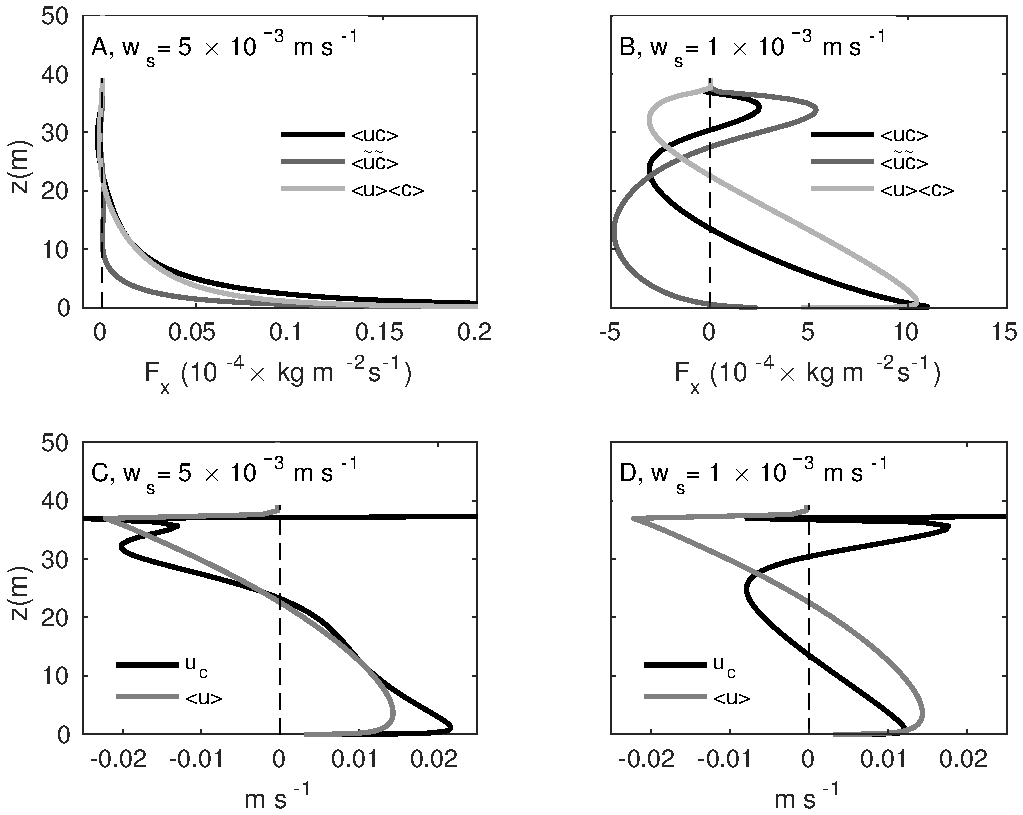
\includegraphics[width=40pc]{restrans.pdf}
  \caption{Residual cross-slope fluxes of suspended material for
    settling velocities (a) $w_s = 5 \times 10^{-3}$~m~s$^{-1}$ and
    (b) $w_s = 1 \times 10^{-3}$~m~s$^{-1}$ with contributions from
    the residual currents and tidal pumping as indicated. Panels (c)
    and (d) show the corresponding effective transport velocities
    defined in (\ref{ucvc}). Note the different axes ranges. }
  \label{residualu}
  
\end{figure}
Figs.\ \ref{residualu} and \ref{residualv} compare cross-slope and
along-slope SPM fluxes for the two sinking speeds shown in
Fig.\ \ref{wsdifference}c,d. As already speculated in section
\ref{temporal}, for the larger sinking speed the contribution of tidal
pumping to the total cross-slope flux is small due to the fact that
high SPM concentrations generally co-occur with negligible cross-slope
speeds (Fig. \ref{residualu}a). This is confirmed by
Fig.\ \ref{residualu}c, showing that the transport velocity $u_c$ is
of the same order of magnitude as the residual current $\langle u
\rangle$. Different from the non-rotating case investigated by
\cite{schulzumlauf2016}, tidal pumping is therefore not the
dominating process in this example. This is also true for the case
with a small sinking speed (Fig. \ref{residualu}b,d), which is,
however, further complicated by the fact that the contributions of the
residual current and tidal pumping may point into different
directions.

\begin{figure}
  \noindent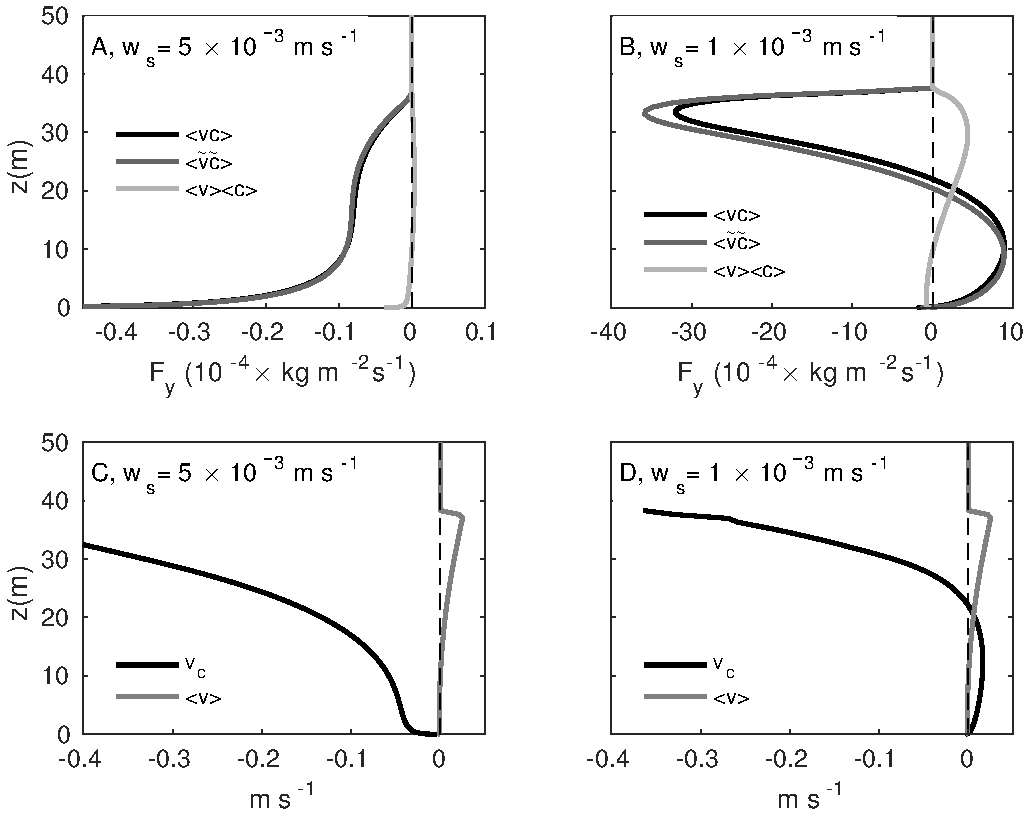
\includegraphics[width=40pc]{restransv.pdf}
  \caption{As in Fig.\ \ref{residualu}, but now for the along-slope
    SPM fluxes and transport velocities. Note that the axes ranges are
    different from Fig.\ \ref{residualu}.}
  \label{residualv}
\end{figure}

The situation changes completely if the along-slope fluxes are
considered. Fig.\ \ref{residualv}a,b shows that for both sinking
speeds tidal pumping provides the overwhelming contribution to the net
SPM fluxes. The strong correlation between large SPM concentrations
and negative along-slope velocities for the case with a large sinking
speed (see section \ref{temporal}) induces a residual flux of
suspended material in the negative $y$-direction that is almost one
order of magnitude larger than the corresponding cross-slope flux
(Fig.\ \ref{residualu}a). The effectiveness of tidal pumping in this
case is corroborated by Fig.\ \ref{residualv}c, showing that the
contribution of the residual current to the effective transport
velocity $v_c$ is generally negligible. Typical transport velocities
in the lower part of the BBL, where SPM concentrations are high, are
of the order of $0.1$~m~s$^{-1}$, suggesting that suspended material
is transported approximately 5~km along the slope during one tidal
cycle.

Particularly notable is the two-layer structure determining the
along-slope SPM transport for the case with a low sinking speed
(Fig.\ \ref{residualv}b), which may be explained as follows. Comparing
the along-slope velocities in Fig.\ \ref{modeloutcome}b and the SPM
concentrations in Fig.\ \ref{wsdifference}d shows that during periods
of positive along-slope flow, near-bottom SPM concentrations are
highest because stable stratification prevents resuspended material to
be diluted by mixing across a larger fraction of the BBL. The opposite
is the case for periods with negative along-slope flow. Here, SPM is
mixed up high into the BBL, because mixing is not suppressed by stable
stratification any more. The net effect of the resulting correlations
is a positive along-slope transport near the bottom, and a negative
transport in the upper part of the BBL.


\subsection{Variable sinking speed and stratification}
To quantify the variability of SPM transport across a larger parameter
space, it is useful to introduce the normalized integrated fluxes,
\begin{equation}
  \label{ucint}
  U_c = \frac{ \int \langle uc \rangle dz}{\int \langle c \rangle dz}
  \; , \quad V_c = \frac{\int \langle vc \rangle dz}{\int \langle c
    \rangle dz} \; .
\end{equation}
Analogous to the vertically variable transport velocities $u_c$ and
$v_c$, the vertically integrated expressions in (\ref{ucint}) define
bulk measures for the residual velocities at which SPM is transported
across and along the slope, respectively \citep{schulzumlauf2016}.

\begin{figure}[ht]
  \noindent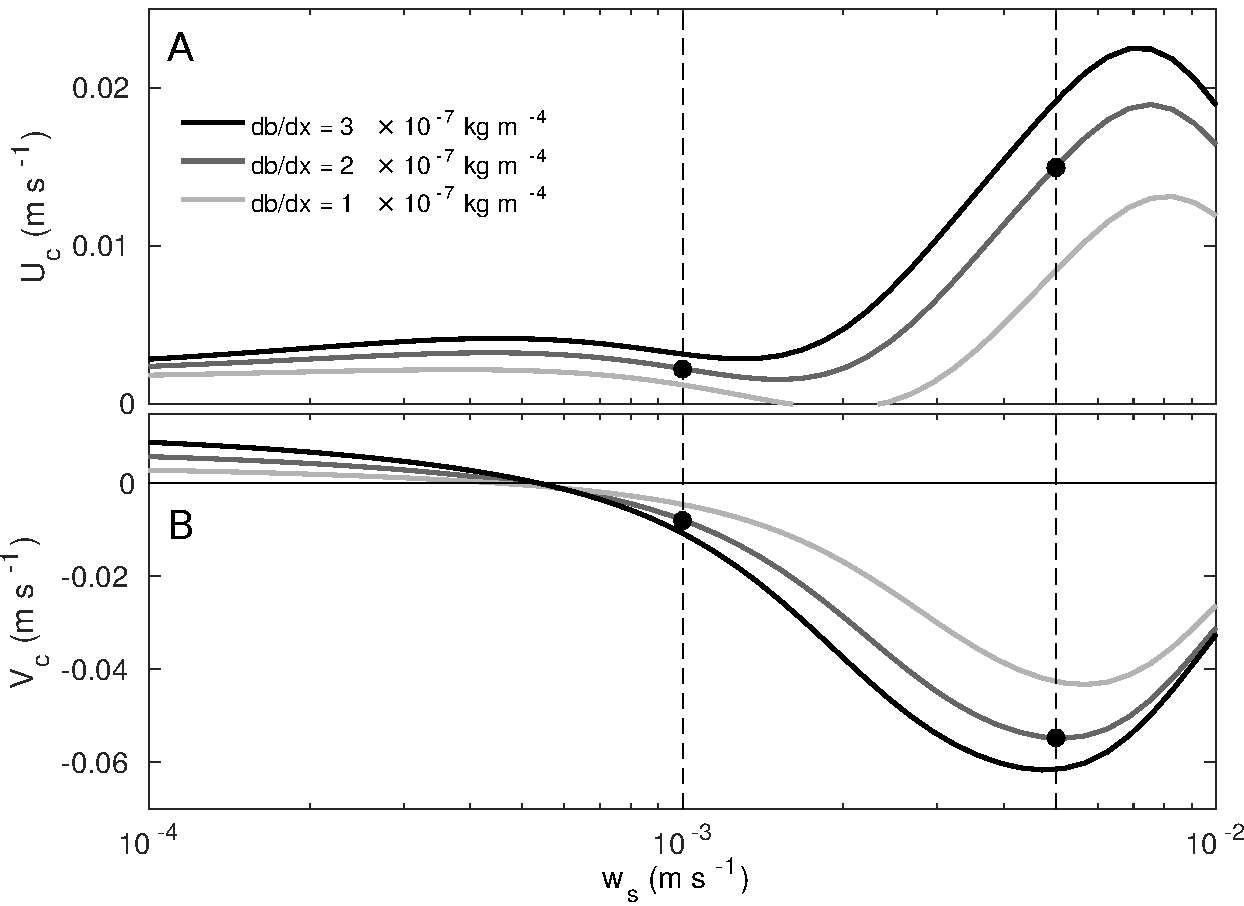
\includegraphics[width=30pc]{wsvariation.pdf}
  \caption{Distribution of (a) cross-slope and (b) along-slope
    transport velocities, $U_c$ and $V_c$, for variable settling
    velocities and cross-slope buoyancy gradients (all other
    parameters as in Tab.\ \ref{input}).  Dashed vertical lines
    indicate the standard cases of small and large settling velocities
    discussed in the context of
    Fig.\ \ref{wsdifference}.}\label{wsvariation}
\end{figure}

In Fig.\ \ref{wsvariation}, the distribution of $U_c$ and $V_c$ for
varying settling velocities is displayed.  As already discussed in
section \ref{residualtransports}, the cross-slope sediment flux is
largely determined by the contribution of the residual current,
$\langle u \rangle \langle c \rangle$, which is directed upslope near
the bottom and downslope in the upper part of the BBL. The
contribution of tidal pumping is either relatively small (for large
sinking speeds, see Fig.\ \ref{residualu}a,c), or even counteracts the
contribution of the residual current (for small sinking speeds, see
Fig.\ \ref{residualu}b,d). The local maximum in $U_c$ for $w_s \approx
7 \times 10^{-3}$~m~s$^{-1}$ (Fig.\ \ref{wsvariation}a) can thus be
explained as follows. For settling velocities higher than this optimal
value, suspended matter remains inside a thin near-bottom layer, where
flow velocities are strongly reduced due to frictional effects. SPM
transport is not efficient in this case. Material that exhibits
settling velocities smaller than the optimal value is more
homogeneously distributed across the BBL, implying that the
near-bottom upslope transport is partly compensated by a downslope
transport in the upper part of the BBL.  The local minimum, visible
Fig.\ \ref{wsvariation}a for sinking speeds slightly larger than
$w_s=10^{-3}$~m~s$^{-1}$, originates from the effect of tidal pumping,
opposing the contribution of the residual current for material with
small settling velocities (see Fig.\ \ref{residualu}b). It is
remarkable that for virtually all settling velocities investigated
here, the transport is directed upslope, similar to the non-rotating
case studied by \cite{schulzumlauf2016}.

Different from the cross-slope transport of suspended material, the
along-slope transport is mainly determined by tidal pumping
(Fig.\ \ref{residualv}). In this case, $V_c$ reaches a local minimum
(maximum negative transport rates) near $w_s \approx 5 \times
10^{-3}$~m~s$^{-1}$. This optimum value is also marked in
Fig.\ \ref{wsvariation}, and corresponds to the case of large sinking
speed discussed in the previous sections. The maximum in the transport
rate for this value of the sinking speed is shaped by two competing
effects. For settling velocities larger than the optimum value,
suspended material is largely located inside the thin frictional
near-bottom layer, where tidal pumping is not effective and $V_c$ thus
decreases. For material sinking slower than the optimal value, the
negative near-bottom transport is partly compensated by an opposing
transport in the upper part of the BBL (see example in
Fig.\ \ref{wsvariation}b). If sinking speeds are small enough, this
effect may even cause a reversal of the transport direction
(Fig.\ \ref{wsvariation}b). Comparing the magnitudes of $U_c$ and
$V_c$ in Fig.\ \ref{wsvariation}, it is evident that along-slope tidal
pumping results in a factor of 2-3 larger transport velocities
compared to the cross-slope direction.

Finally, it is worth noting that Fig.\ \ref{wsvariation} also reveals
that stronger background stratification enhances the SPM transport
mechanisms in both the cross-slope and along-slope directions. This is
little surprising, however, as stratification is one of the
prerequisites for slope-induced tidal straining and pumping. The
existence of an optimal settling velocity for up-slope transport, and
the observed dependency on background stratification, are in agreement
with the findings of \cite{schulzumlauf2016} for the non-rotating
case.



\subsection{Rotational effects}

According to (\ref{Un}) and (\ref{Us}), the shape of the tidal ellipse
is determined by the Coriolis parameter, which is therefore likely to
have an important impact on tidal straining and SPM transport. In the
following, we investigate this effect in a series of simulations with
varying latitude (varying Coriolis parameter), leaving all other
parameters as in Tab.\ \ref{input}. For the sinking speed, we assume
$w_s=5 \times 10^{-4}$~m~s$^{-1}$, corresponding to the optimal value
for along-slope tidal pumping identified in the previous section.

We consider two special cases for the pressure forcing in
(\ref{Pn}). In the first case, we assume that the pressure force is
directed exactly in the cross-slope direction ($P_x \neq 0$, $P_y=0$),
whereas in the second case the forcing is purely along-slope ($P_x =
0$, $P_y \neq 0$). Using the analytical solution in (\ref{Un}), we
adjust the pressure force $P$ for each case exactly such that the
velocity amplitude in the direction of the forcing remains constant at
a value of 0.5~m~s$^{-1}$. This results in a tidal ellipse with the
(constant) major axes oriented parallel to the pressure force (i.e.,
either cross-slope or along-slope), and the minor axes increasing in
magnitude with increasing Coriolis parameter. The latter is varied by
changing the latitude from 20$^\circ$~N to 60$^\circ$~N at 10$^\circ$
intervals, corresponding to axes ratios between 0.35 and 0.89 for the
tidal ellipses.  Using (\ref{omegacjgr}), it is easy to show that for the
parameters in Tab.\ \ref{input}, BBL resonance and the transition to
super-critical slopes \citep[see][]{schulzumlauf2016} occur at a
latitude of approximately 75$^\circ$~N. The range of latitudes used
here guarantees that BBL resonance does not affect the results.

\begin{figure}
  \noindent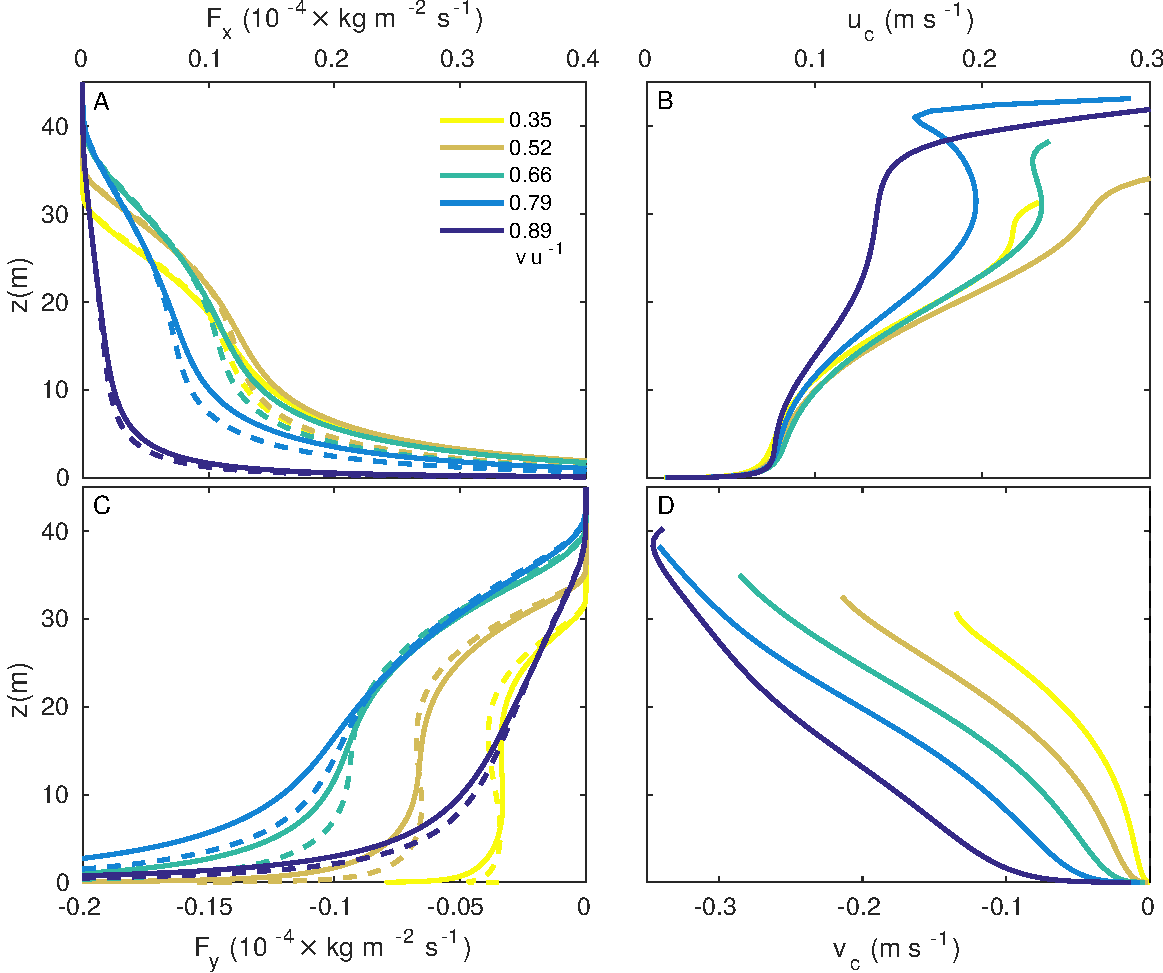
\includegraphics[width=30pc]{coriolis.pdf}
  \caption{Profiles of (a) cross-slope and (c) along-slope SPM flux,
    and (b) cross-slope and (d) along-slope transport velocity for a
    range of latitudes between 20$^\circ$~N and 60$^\circ$~N (at
    10$^\circ$ intervals).  The pressure forcing is purely cross-slope
    ($P_y=0$), and the amplitude of the cross-slope tidal velocity
    fluctuations in the region above the BBL is $u=0.5$~m~s$^{-1}$ for
    all cases. The amplitude of the corresponding along-slope
    component $v$ increases with latitude as indicated.  Dashed lines
    in (a) and (c) show the contribution of tidal pumping to the
    overall SPM flux.}
  \label{coriolis}
\end{figure}

The case with pure cross-slope forcing ($P_y=0$) includes the
non-rotational case ($f=0$, $v=0$) investigated in detail by
\cite{schulzumlauf2016}. As pointed out by these authors, the
turbulent diffusivities show in this case a clear $M_4$ signal that
exhibits a $M_2$ modulation due to SIPS (higher diffusivities are
observed during periods with upslope flow). These tidal asymmetries
trigger an efficient tidal pumping mechanism that transports suspended
material in the upslope direction. Fig.\ \ref{coriolis}a,b shows that
this mechanism remains essentially unchanged for latitudes up to
approximately 40$^\circ$~N, corresponding to a axis ratio of 0.66 for
the tidal ellipse. While the BBL thickness significantly increases
over this range of latitudes, SPM fluxes and transport velocities
exhibit only small changes in the lowest 20~m of the BBL, where most
of the suspended material is located and therefore most of the
transport occurs. Quite differently, the along-slope SPM transport,
vanishing for $f=0$, quickly increases for $f>0$ as a result of the
same tidal pumping mechanisms described in detail in sections
\ref{temporal} and \ref{residualtransports} (see
Fig.\ \ref{coriolis}c,d).

\begin{figure}
  \noindent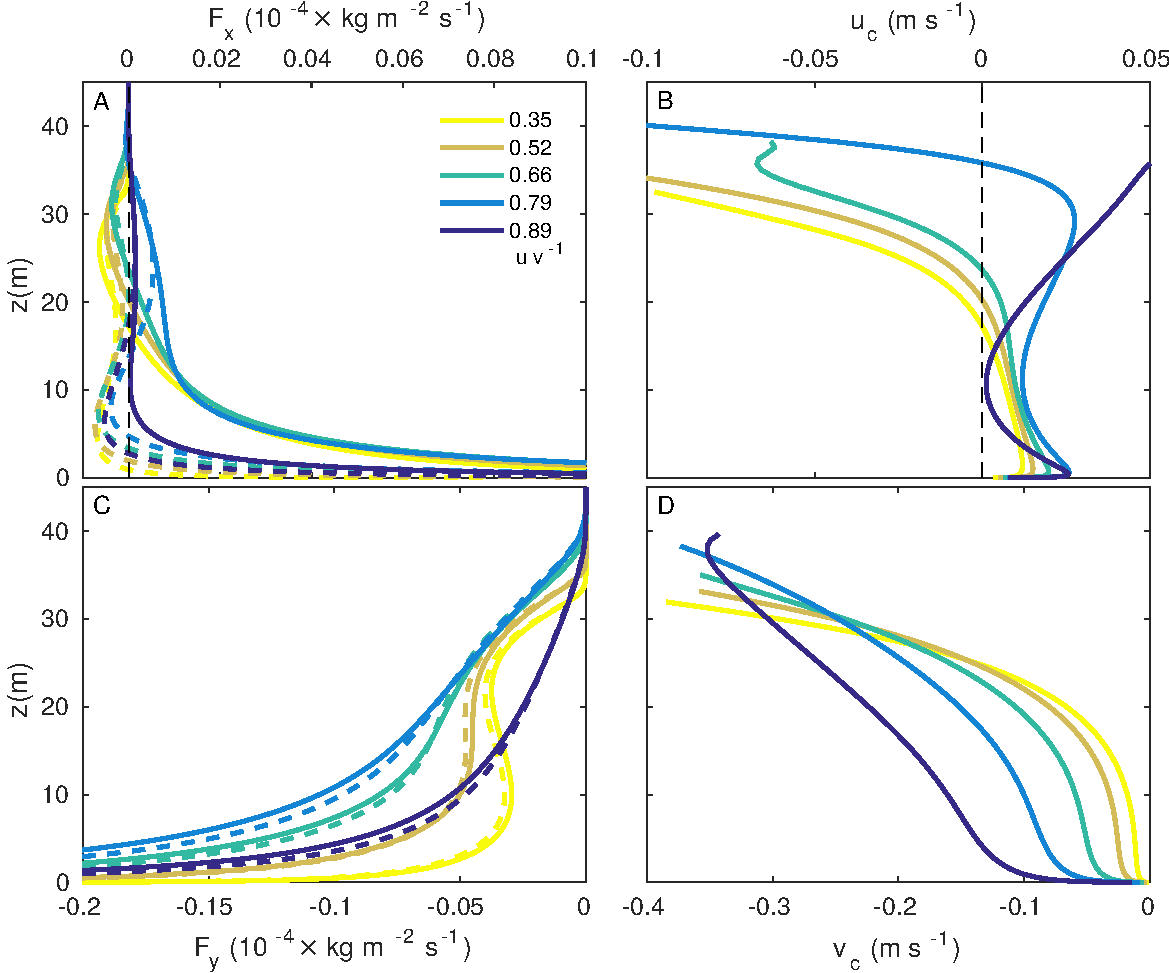
\includegraphics[width=30pc]{coriolis2.pdf}
  \caption{As in Fig.\ \ref{coriolis}, but now for along-slope
    pressure forcing ($P_x=0$), and constant amplitude of the
    along-slope tidal velocity fluctuations ($v=0.5$~m~s$^{-1}$).}
  \label{coriolis2}
\end{figure}

For higher latitudes, the tidal ellipses gradually approach a circular
shape, implying that the magnitude of the rotating velocity vector
changes only slightly during a tidal cycle. As consequence, the
turbulent diffusvity and the bottom stress (both important for SPM
erosion) show a transition from a pronounced $M_4$ variability with
two maxima during a tidal cycle towards a weak $M_2$ modulation with a
single maximum during periods with upslope flow. Considerably less
material is eroded during this single maximum compared to the cases
with smaller rotation rates, and SPM concentrations strongly
decrease. Therefore, although tidal pumping is still active or even
increasing in the along-slope direction (see Fig.\ \ref{coriolis}d),
the total SPM fluxes collapse for high latitudes
(Fig.\ \ref{coriolis}a,c).

In our second series of simulations, we assume that the tidal pressure
force is directed exactly along the slope ($P_x=0$). Different from
the case with cross-slope forcing, both the cross-slope and the
along-slope SPM fluxes vanish in the limit $f \rightarrow 0$ for
symmetry reasons. For increasing latitudes, a weak upslope transport
develops, which, similar to the example in section
\ref{residualtransports}, is driven by the residual flow rather than
by tidal pumping (Fig.\ \ref{coriolis2}a,b). The weak transport rates
in the cross-slope direction are strongly contrasted by the vigorous
along-slope tidal pumping mechanism that quickly develops for
increasing $f$ (Fig.\ \ref{coriolis2}c,d). The mechanisms are analogous
to the example discussed in the previous sections (see
Fig.\ \ref{residualv}a,c), which was also characterized by a dominant
along-slope flow component. For the highest latitudes, however, both
the cross-slope and along-slope transports collapse again due to
decreasing concentrations of suspended material. The reasons are
identical to those discussed above.

\section{Conclusions} \label{conclusions}
Two main conclusions can be drawn from the first part of our study,
which showed that an idealized one-dimensional numerical model is able
to reproduce the most important features in a dataset describing tidal
straining on a sloping shelf in the East China Sea. First, the good
agreement between model and data indicates that the model correctly
represents the key physical processes determining slope-induced tidal
straining; and secondly, our results let it seems unlikely that
processes other than those represented in the model (e.g., classical
tidal straining due to river runoff) explain the observed BBL
variability at our study site. The combination of model results and
experimental data therefore provides the first direct and conclusive
evidence for the occurrence of slope-induced tidal straining at a real
ocean site.

Our simulations also revealed a number of important processes related
to the effect of rotation, which was ignored in previous studies of
slope-induced tidal straining. For tidal ellipses oriented in the
cross-isobath direction, the upslope transport of suspended material
by tidal pumping, originally described by \cite{schulzumlauf2016} for
the non-rotating case, was only slightly modified by rotational
effects. However, the along-slope tidal velocity fluctuations induced
by these rotational effects were shown to trigger a new type of tidal
pumping mechanism that efficiently transports suspended material along
the slope. A comparable along-slope tidal pumping was also observed
for tidal ellipses oriented with their main axes along isobaths. In
both cases, tidal pumping was found to be most efficient for an
optimal sinking speed that was of the order of $5 \times
10^{-4}$~m~s$^{-1}$ in our example. For material sinking significantly
slower or quicker than this value, the tidal pumping of suspended
material was strongly reduced. Typical transport velocities deduced
from our simulations suggest that suspended material may be
transported over several kilometers along the slope during one tidal
cycle.

%% In this case, however, it also turned out that rotational effects tend
%% to decorrelate cross-slope tidal fluctuations in velocity,
%% $\tilde{u}$, and SPM concentration, $\tilde{c}$, thus resulting in a
%% shut-down of upslope tidal pumping ($\langle \tilde{u} \tilde{c}
%% \rangle \rightarrow 0$). Cross-slope transport in this situation is
%% determined by the contribution of the residual circulation $\langle u
%% \rangle \langle c \rangle$, which is, however, a much less efficient
%% mechanism.


Additional parameter studies have shown that the processes identified
in this study are robust, and therefore likely to occur across a wide
range of naturally occurring conditions. In contrast to classical tidal
straining that relies on the existence of a freshwater source or
differential heating, slope-induced tidal straining only requires: a
slope, an oscillating tidal current, and a stratified water
column. These pre-requisites are nearly ubiquitous in the ocean.

\chapter{The Baltic Sea}
\label{kap-einleitung}

In the previous chapters, an idealized process study with the help of a 
numerical model was carried out (section \ref{kap-slope}) and observations of 
the discussed process in an existing data set from the East China Sea were 
reproduced (section \ref{kap-jgr}). Besides model studies, several field work 
campaigns were performed in the context of this thesis. The measurements were 
carried out in coastal areas of the Western Baltic Sea. Prior to the discussion 
of the obtained data in the next chapter, an introduction on the evolution of 
the Baltic Sea and the present hydrological conditions is given in this 
chapter, and the sedimentology and prevailing hydrodynamic processes which are 
characteristic in parts of the Western Baltic Sea are highlighted.

\section{History and Present State}

The Baltic Sea emerged from a subglacial lake at the end of the Weichselian Ice 
Age, approximately 12,000 BP, and has since gone through several stages of 
salty and brackish sea states or fresh water conditions, depending on whether a 
connection to the open ocean was established or not. Indicators for this 
alternations are, amongst others, changes in the benthic communities, and so the 
nomenclature of the evolution stages was often determined by the prevailing 
species.

With the retreat of the glaciers at the end of the Weichselian Ice Age, a 
subglacial lake, together with water from the rapidly melting glaciers, formed 
the \textit{Baltic Ice Lake}. Land uplift, that followed the deglaciation, 
formed a landbridge between Sweden and the main land 11,200 BP, damming the 
Baltic Ice Lake. Sea level was raised by glacial melt water until the lake began 
to drain over the Öresund sill. Presumably, a lowering of the water level by 25 
to 28 m by drainage through a channel near Mt. Billingen in central Sweden 
happened very rapidly around 10,300 BP, when the retreating ice margin collapsed 
\citep[][]{bjoerk95,tikkanen2002} and a connection to the sea was opened. 

This new stage of the Baltic with a lower sea level is known as \textit{Yoldia 
Sea} (from the marine mollusc \textit{Portlandia (Yolida) arctica} 
\citep[][]{schoning2001}). There are no indicators for salt water entrainment 
into the Yoldia Sea until global sea level rise and deglaciation formed a 
connection through the Närke Strait 300 years later \citep[][]{schoning2001}. 
This lead to brackish water conditions followed by decreasing salinity after the 
straits had become too narrow to allow water exchange another 100 to 300 years 
later \citep[][]{bjoerk95}.

After the glaciers retreated, uplift of the land was not be compensated by 
global sea level rise. Connection to the ocean was closed again around 9,500 BP, 
and the regime shifted to fresh water conditions again, now called 
\textit{Ancylus Lake} (after the freshwater gastropod \textit{Ancylus 
fluviatilis} \citep[][]{tikkanen2002}). Although narrow outlets existed, the 
surface of the Ancylus Lake rose up to 10 m above global sea level, inundating 
extensive areas of land. This phase, called the Ancylus Transgression, ended 
around 9,200 BP, when the sea level height exceeded the height of the Darss Sill 
and water began to flow out through an evolving river system in the land 
connection between Sweden and Germany \citep[][]{tikkanen2002}. Around 9,000 BP 
this so-called Ancylus Regression ended when the water level reached global sea 
level. The connection to the ocean through the river system remained, but no 
extensive saline intrusion happened for the next 1,000 years.

Ongoing global sea level rise deepened the connection between the Baltic Basin 
and the open ocean, letting more and more saline water enter the Ancylus Lake. A 
short transition stage called \textit{Mastogloia Sea} (\textit{Mastogloia} are 
diatoms that live in slightly saline conditions \citep[][]{eronen2001}) was 
followed by the \textit{Litorina Sea} (named after the brackish water gastropod 
\textit{Littorina littorea} \citep[][]{eronen2001}), when a great extent of 
saline water entered the Baltic basin through the Straits of Denmark in 7,500 BP 
\citep[][]{bjoerk95}. Transgression took place until the rise in ocean levels 
ended 6,000 to 5,000 BP. When the Straits of Denmark became shallower, as land 
uplift continued, water exchange was reduced and salinity in the Litorina Sea 
declined down to the present brackish state in 4,000 BP, at first named 
\textit{Limnea Sea} (from the snail \textit{Lymnaea ovata}), and finally, since 
500 BP, \textit{Mya Sea} (after the Northern American clam \textit{Mya 
arenaria}, which was brought into the Baltic by Viking ships 
\citep[][]{bjoerck2008}).

\begin{figure}[ht]
 \flushleft
 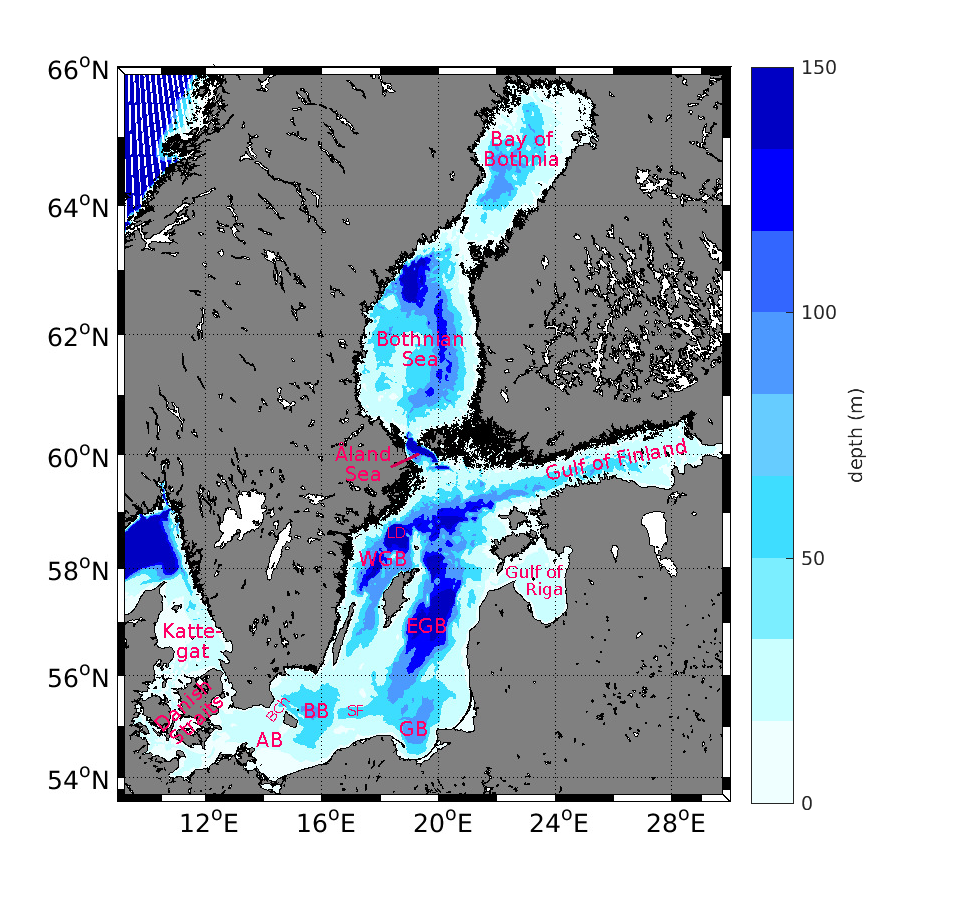
\includegraphics[width=17cm]{bilder/baltic.pdf}
 \caption{Topographic map of the Baltic Sea. Abbreviations stand for Arkona 
Basin (AB), Bornholm Channel (BCh), Bornholm Basin (BB), S\l upsk Furrow (SF), 
Gda\`{n}sk Basin (GB), Eastern Gotland Basin (EGB), Landsort Deep (LD) and 
Western Gotland Basin (WGB).}\label{balticmap}
\end{figure}

Today, the Baltic Sea has an extent of $4.2 \times 10^{5} \, \text{km}^2$ 
\citep[][]{balticsea} and is connected to the North Sea via the Danish Straits: 
the \O resund and the Great and Little Belt together with the Fehmarn Belt. The 
climate is humid: Annual precipitation adds around 224 $\text{km}^3$ of water to 
the Baltic Sea, evaporation amounts to only 184 $\text{km}^3$. River discharge a 
total of 436 $\text{km}^3$ water per year. \citep[][]{reissmann2009}. An 
exchange flow takes place, where brackish water leaves the Baltic near the 
surface (annually around 947 $\text{km}^3$) and saline North Sea water enters at 
the bottom (nearly 500 $\text{km}^3$ a year on average, but frequency and 
strength of inflow events differ dramatically over time, highly dependent on 
short term weather conditions). Two shallow sills, the Dr\o gden Sill (7 m deep, 
values in brackets refer to the local depth in the following) and the Darss Sill 
(18 m) form the passage to the first of several basins, the Arkona Basin (45 m), 
through which the North Sea water propagates as a deep gravity current 
(see \fig{balticmap}). Through 
the Bornholm Channel, the Arkona Basin is connected to the Bornholm Basin (80 
m), from where the bottom current flows over the S\l upsk Sill (60 m) and 
through the approximately 80 km long S\l upsk Furrow (90 m) southeast into the 
Gda\`{n}sk Basin (110 m) and northeast into the Eastern Gotland Basin (250 m). 
From there, the deep current can enter the easterly Gulf of Riga or the Western 
Gotland Basin, wherein the Landsort Deep (with 490 m the deepest point in the 
Baltic Sea) is located. The Gulf of Finnland forms the eastern boundary of the 
Baltic Sea and north of the Gotland Basin, the \r{A}land Sea separates the 
Baltic Proper in the south from the Bothnian Sea and the Bay of Bothnia in the 
north \citep[][]{reissmann2009}. Salt water entering at the Darss Sill needs 
approximately 2--6 months to exchange the bottom water in the Gotland Basin 
\citep[][]{balticsea}.

The bathymetry of the Baltic Basin together with climate conditions and the 
exclusive water exchange via the Danish Straits leads to several notable 
features in the hydrographic conditions: Dense bottom water from the North Sea 
creates a permanent strong halocline that separates bottom from surface water, 
preventing ventilation of the water masses in the deep basins. Oxygen that 
enters through exchange with the atmosphere is not mixed below the halocline, 
leaving entraining North Sea water the only oxygen source. Large parts of the 
Baltic Sea become anoxic after long periods without significant salt water 
inflows, with severe implications on geochemical processes and the ecosystem of 
both the lower water column and the sediment-water interface. 

Since the only source of saline water are inflows from the North Sea, a 
salinity gradient is present across the Baltic Sea: The bottom current is 
entrained with overlying brackish water along its pathway (for example, volume 
of the gravity current increases by 53 \% when passing through the Arkona Basin, 
\citep[see][]{reissmann2009}), and slow entrainment of salt into the overlying 
water mass forms a NE--SW surface salinity gradient. Surface salinity drops from 
around 18 psu in the Danish Straits to 8 psu in the Arkona Basin, down to 6--7 
psu in the Eastern Gotland Basin and even below 3 psu in the Bay of Bothnia and 
the Gulf of Finnland \citep[][]{balticsea}.

WAVE CLIMATE AND INERTIAL OSCILLATIONS GENERATION!

\section{Major Baltic Inflow December 2014}

GANZES KAPITEL WEG?

Saline water can enter the Baltic Sea in two different ways. Baroclinic inflows 
are triggered by the horizontal salinity gradient between North and Baltic Sea 
and occur at calm wind conditions, mostly in summer \citep[][]{reissmann2009}. 
The main impact on the ventilation of the deep sea is, however, subject to the 
barotropic inflow events, called Major Baltic Inflows (MBIs). Those MBIs occur 
irregularly and are caused by special meteorological conditions: Firstly, high 
air pressure over the Baltic region and strong winds in westerly direction cause 
the mean sea level in the Baltic to drop by up to 50 cm, imposing a gradient in 
sea level elevation between Kattegat and Arkona Basin. Secondly, several weeks 
of wind in easterly direction with strong gales \citep[][]{balticsea, 
reissmann2009, mohrholz2015} push saline and oxygen rich water into the Baltic 
Sea.
These conditions occur primarily between October and February. Since records 
started in 1897, MBIs were on a rather regular base up to the 1970s. After this, 
long periods without inflow events decreased oxygen supply in the Baltic basins 
drastically. The last MBIs were in 1993 and 2003, but they interrupted the 
anoxic conditions in the deep water only for short periods of time 
\citep[][]{schinke1998, mohrholz2015}.

In November 2014, medium to strong easterly winds forced an outflow of Baltic 
sea water and consequently a drop in mean sea level of 57 cm. At the beginning 
of December, the wind changed to heavily westerly wind, pushing a strong 
barotropic inflow of saline water into the Baltic Sea. The main inflow period 
lasted until Christmas. During that time, an overall amount of 320 $\text{km}^3$ 
water was imported into the Baltic Sea, carrying approximately 4 Gt salt. The 
MBI in 2014 was the third largest inflow event recorded since 1880 and has the 
potential to ventilate the entire deep water of the Baltic. 

\section{German Coastal Seas and Sediment}

General sedimentology and grain size distribution of parts of the Western 
Baltic Sea have 
been mapped in detail in a collaboration between the German maritime and 
hydrographic agency (BSH) and the Leibniz Institute for Baltic Sea Research 
(\fig{westernbaltic}). Prevailing sediments in this area reach from 
fine sand to silt. Although sediment distribution is rather inhomogeneous, some 
features related to the bathymetry are clearly visible. In the very shallow 
regions with water depth less than 20 m, predominately sandy sediments are 
found, while in the deeper basins finer silt is present.
As fine grained material is easily eroded, it is not likely to remain in highly 
energetic, shallow regions and is therefore transported into the deeper basins, 
where 
it accumulates \citep[][]{basys1}. This process is best visible at the 
transition from the Oder Bight to the Arkona Basin. It was found that the 20 m 
isobath separates erosional from depositional areas, and the muddy sediments 
accumulate below a regional halocline here \citep[][]{basys2}. MORE ON THE 
TW and AB REGION. TAUC ETC

\begin{figure}[ht]
 \flushleft
 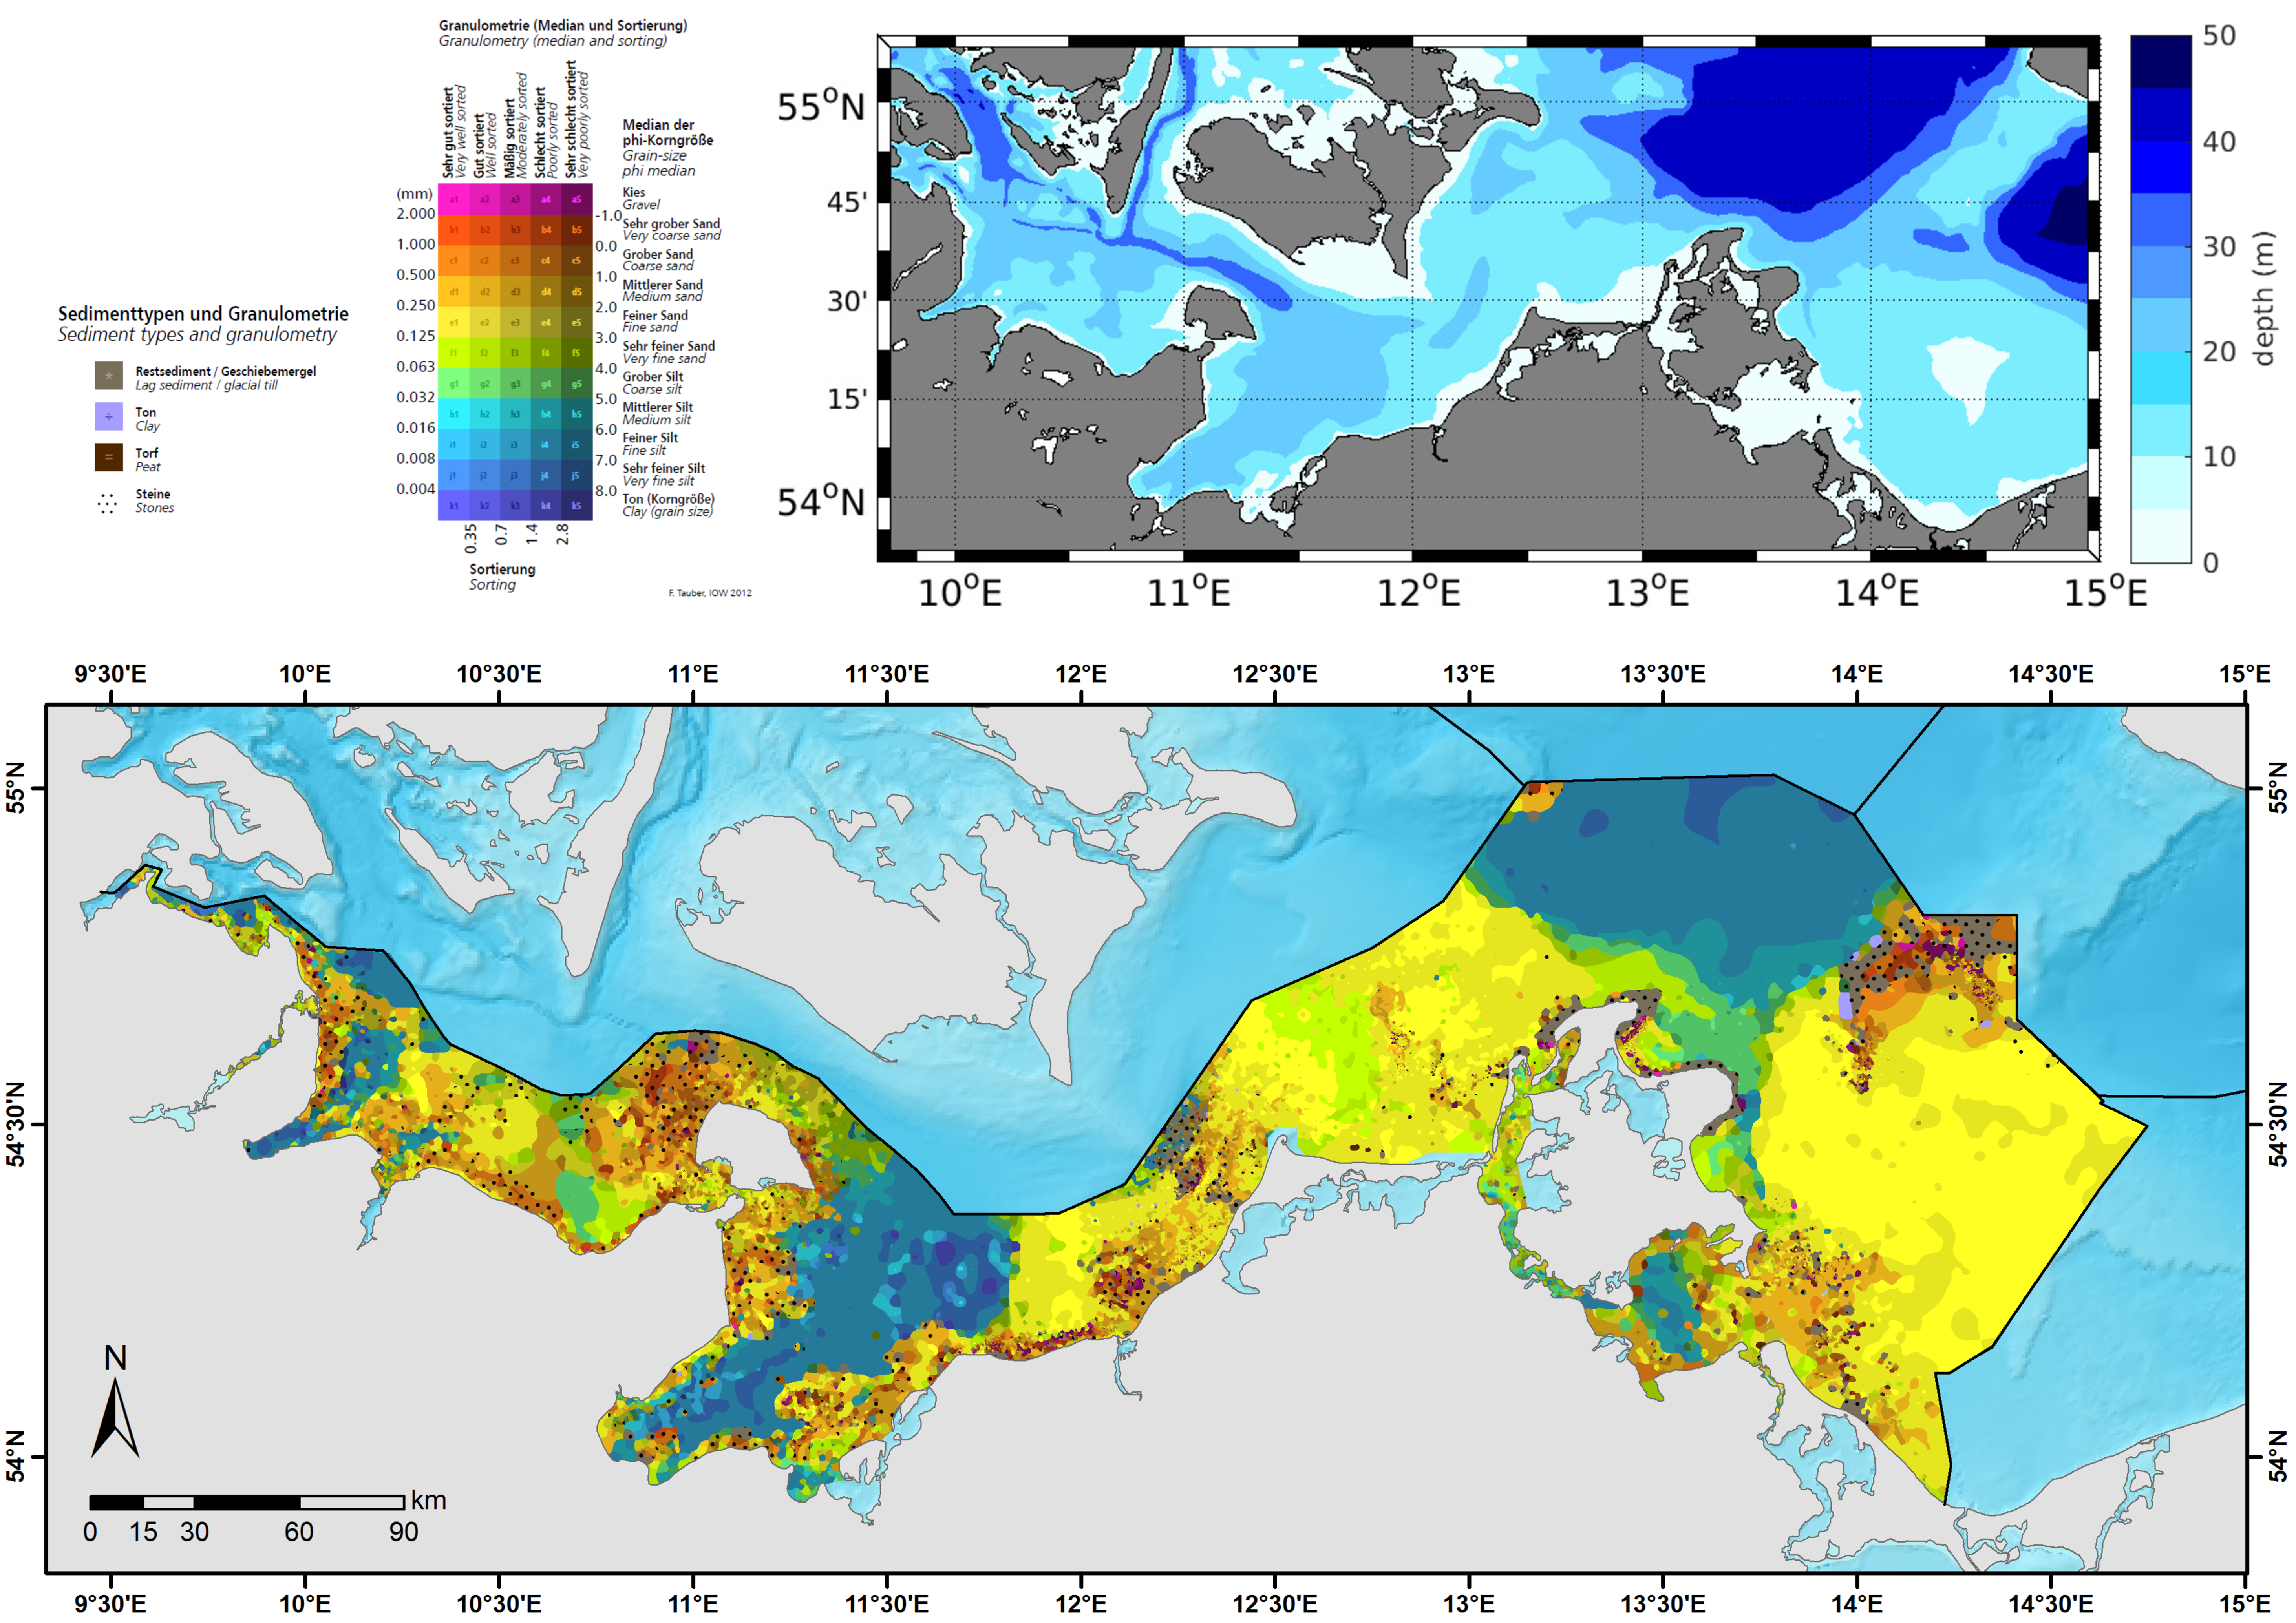
\includegraphics[width=15cm]{bilder/sediment.pdf}
 \caption{Topographic and sediment map of the Western Baltic 
Sea. Sediment data taken from \citep[][]{tauber2012}}\label{westernbaltic}
\end{figure}
\chapter{Measurements}
\label{kap-measure}

\section{Introduction}

\section{Study Area and Instrumentation}

We obtained hydrographic and turbulence data at 
several locations throughout the German coastal area during three cruises with 
R/V \textit{Alkor} in spring 2014 (AL434, 28.03.-08.04.2014), R/V 
\textit{Elisabeth Mann Borgese} in spring 2015 (EMB100, 09.04.-16.04.2015) and 
R/V \textit{Maria S. Merian} in winter 2016 (MSM50, 05.01.-29.01.2016). Here, 
we exclusively discuss data obtained in the transition zone from the coast off 
the island R\"{u}gen (called Tromper Wiek (TW), around 30~m water depth) to 
the approximately 45~m deep Arkona Basin (AB). The exact positions of deployed 
moorings and ship-based microstructure profiler transects are indicated in 
\fig{studyarea}.
 \begin{figure}[ht]
 \centering
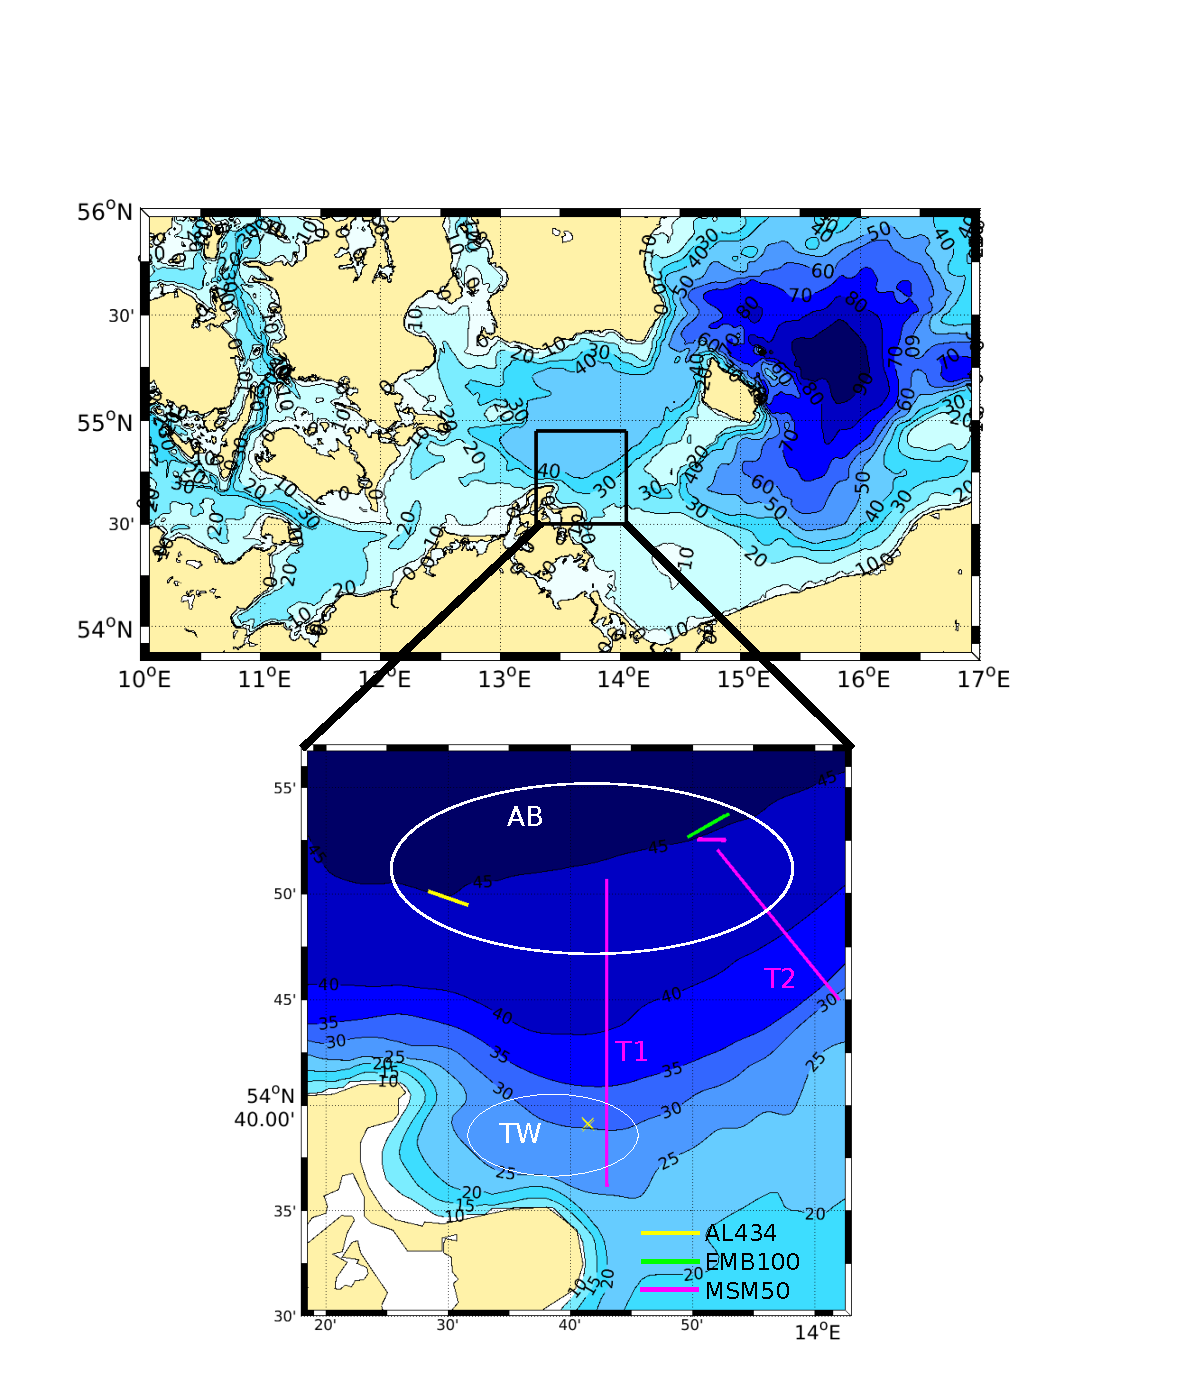
\includegraphics[width=17cm]{bilder/studyarea.pdf}
 \caption{Bathymetric map of the Western Baltic Sea and an enlargement of the 
study area. Deployments during cruise AL434 are indicated in yellow, from EMB100 
in green and from cruise MSM50 in magenta.}
 \label{studyarea}
 \end{figure}
 
 \begin{figure}[ht]
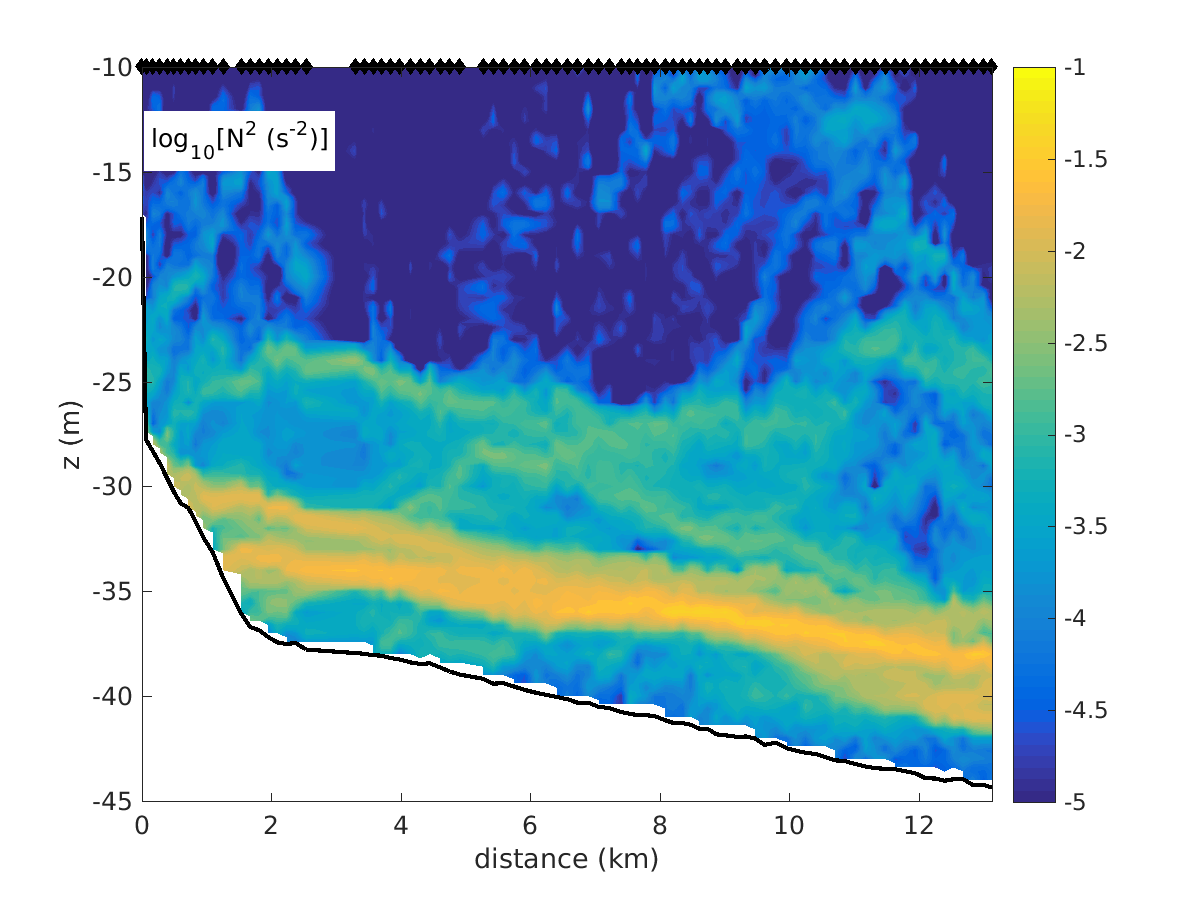
\includegraphics[width=40pc]{bilder/abslope.png}
 \caption{Topographic and hydrologic structure in the study area obtained from 
microstructure transect T1 in 2016. The steep slope on the left hand side has 
an inclination of approximately $5 \times 10^{-3}$, the mild slope further to 
the right of around $7 \times 10^{-4}$. Color indicates the buoynacy frequency 
$N^2$.}
 \label{abslope}
 \end{figure}

 Sediment distribution in this area is heterogeneous in the shallow regions 
with predominately medium to fine sand. At water depths below 25 - 30~m in the 
Arkona Basin, sediment is finer and consists homogeneously of silt 
(\fig{tauberkarte}). In the vicinity of TW, a special type of fine grained and 
organic poor sediment is found. Previous studies \citep[][]{leipe2000, 
basys1} found the Arkona Basin to be a deposition center for material 
orginiating from the shallower areas, with accumulation rates of around 2.2 
mm/yr. Sediment characteristics in the Arkona Basin resemble to those of a 
fluffy layer, i.e. it is easily resuspended and, due to its low settling 
velocity, remains suspended for a relatively long period of time. A consecutive 
study \citep[][]{basys2} found the 20~m isobath to be the border between 
erosional and depositional sites in this area, yielding that the Tromper Wiek 
region is depositional as well. This study also pointed out that muddy 
sediments accumulated below the halocline in this region.
 \begin{figure}[ht]
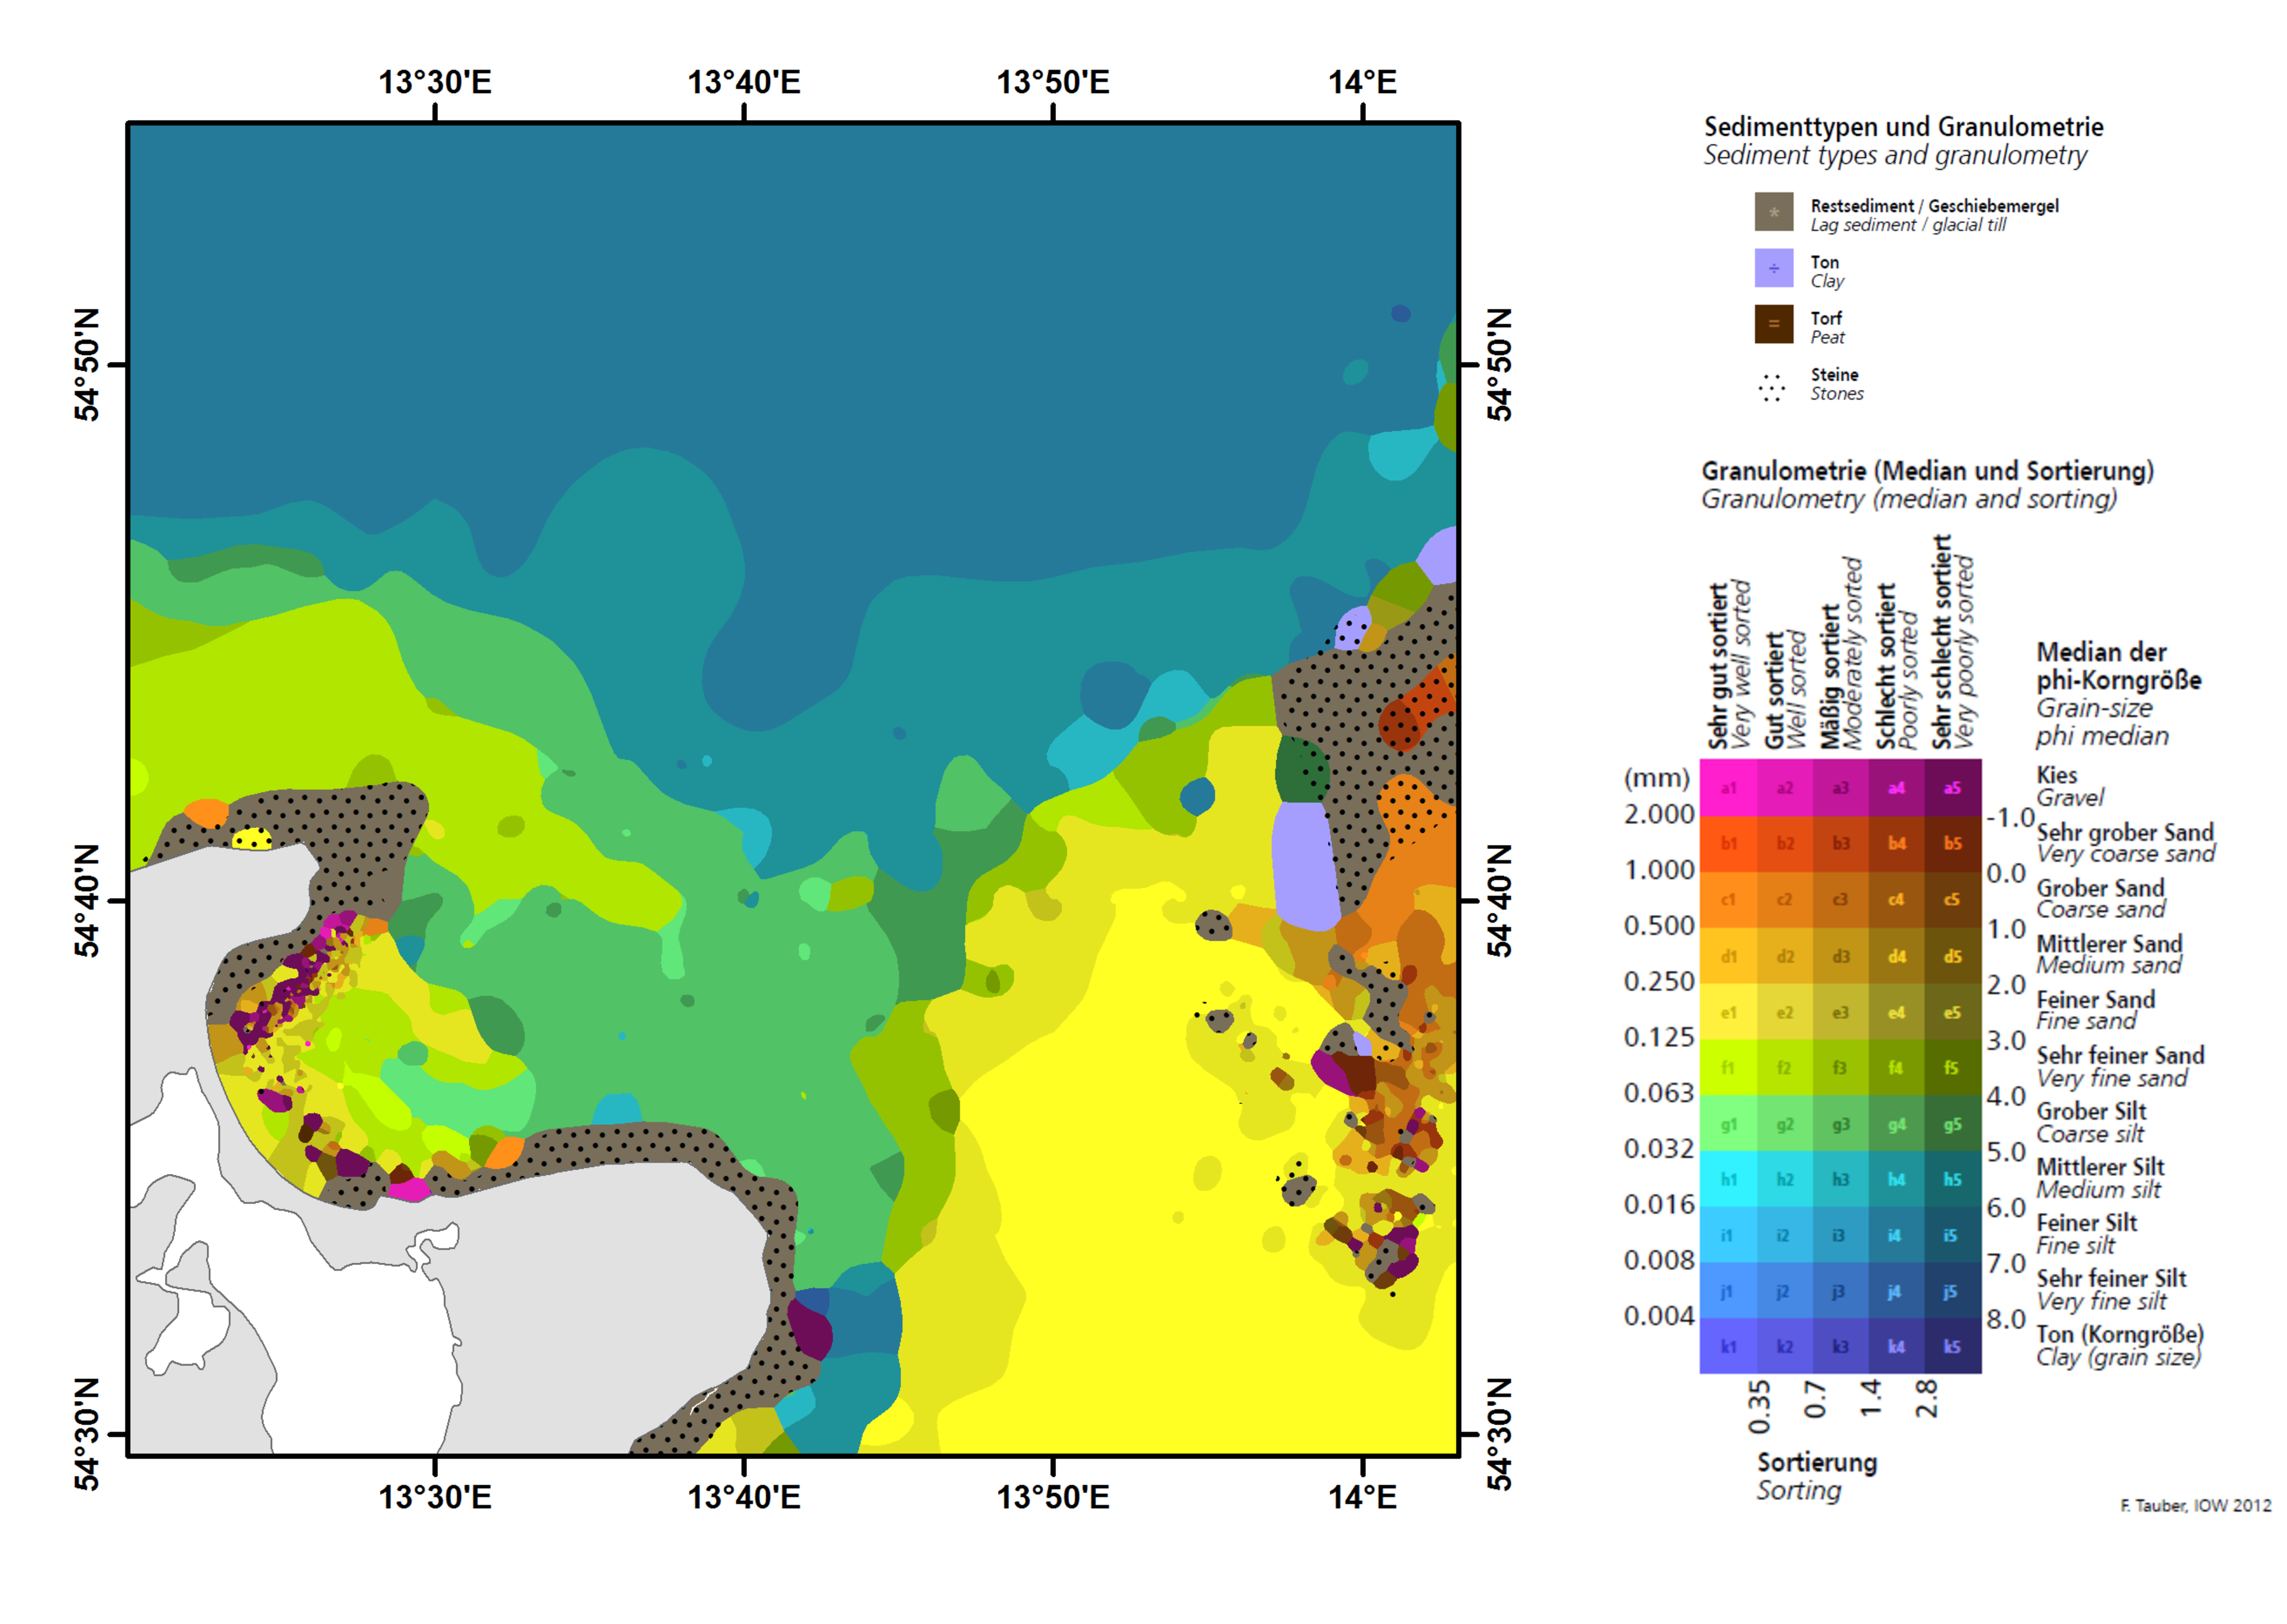
\includegraphics[width=40pc]{bilder/TW.pdf}
 \caption{Sediment distribution in the study area. Data were taken from 
\cite{tauber2012}.}
 \label{tauberkarte}
 \end{figure}

Three different types of moorings were deployed: A CTD-Chain consisted of eight 
CTD-loggers (MicroCat from Seabird, USA), tied to a mooring line at intervals 
of 1 m, starting at 1 m above the seabed, additionally two optical 
backscatter sensors (NTU from Wetlabs, USA) at 3.5 and 5.5 m above the seabed. 
For the EMB100 cruise, the CTD-Chain was extended to 10 CTD-loggers (5 MicroCat 
and 5 TR-1060 type from RBR, Canada) and the turbidity sensors were omitted. 
Lander 1 was a bottom-mounted instrument frame with an upward looking 1200 kHz 
ADCP (Teledyne RDI, USA), a 6 MHz single-point Doppler current meter (Vector 
from Nortek AS, Norway), another CTD-logger and a turbidity sensor. Lander 2 
was a similar bottom frame equipped with an upward looking 600 MHz ADCP 
(Teledyne RDI, USA) and an upward looking 1 MHz (2 MHz during cruise AL434) 
pulse-coherent ADCP (Aquadopp HR from Nortek AS, Norway). For the cruises 
EMB100 and MSM50, Lander 2 was complemented with an additional CTD-logger and a 
turbidity sensor. Deployment times of the moorings are listed in 
\tab{deployments}.

 \begin{table}
\caption{Deployment times of moorings (UTC). In the first 
line, TW and AB indicate deployment sites near the coast and in the Arkona 
Basin, respectively.}\label{deployments}
\begin{center}
\begin{tabular}{cccc}
 & AL434 (TW) & EMB100 (AB) & MSM50 (TW) \\
 \hline
 start & 03.04.2014, 07:00 & 14.04.2015, 12:00 & 26.01.2016, 22:00 \\ 
 end & 08.04.2014, 06:00 & 17.04.2015 04:00 & 28.01.2016, 07:00 \\
\hline
 & CTD-Chain & CTD-Chain & \\
 & Lander 1 & Lander 1 & Lander 1\\
 & Lander 2 & Lander 2 & Lander 2\\
\end{tabular}
\end{center}
\end{table}

Ship-based microstructure measurements were performed with a MSS90-L 
microstructure profiler (ISW, Germany). The instrument contained a set of 
precision CTD sensors, a fast FP07 thermistor, a turbidity sensor, and two 
airfoil shear-probes. During the transects (each of 1 to 5 hours duration) the 
ship moved at 1-2 kn and profiles were obtained continously. Number and time of 
the transects for each cruise are summarized in \tab{mss}.

 \begin{table}
\caption{Start and end times (UTC) and number (in brackets) of microstructure 
transects.}\label{mss}
\begin{center}
\begin{tabular}{cccc}
 & AL434 (2014) & EMB100 (2015) & MSM50 (2016)\\
 \hline
Tromper & 04.04., 16:15 - & & 27.01., 00:00 - \\ 
Wiek & 04.04., 22:30 (4) & & 28.01., 06:00 (9)\\
 & 06.04., 17:30 & & \\
 &  07.04., 22:15 (8) & & \\
\hline
Arkona & 05.04., 16:15 - & 14.04., 16:45 - & 23.01., 13:30 - \\
Basin & 06.04., 01:15 (5) & 15.04., 05:30 (5) & 24.01., 16:45 (7)\\
\hline
transect &  & & 24.01., 19:30 - 23:45 (T1)\\
coast to basin & & & 28.01., 09:45 - 17:00 (T2)\\
\end{tabular}
\end{center}
\end{table}

\section{Observations}

 \begin{figure}[ht]
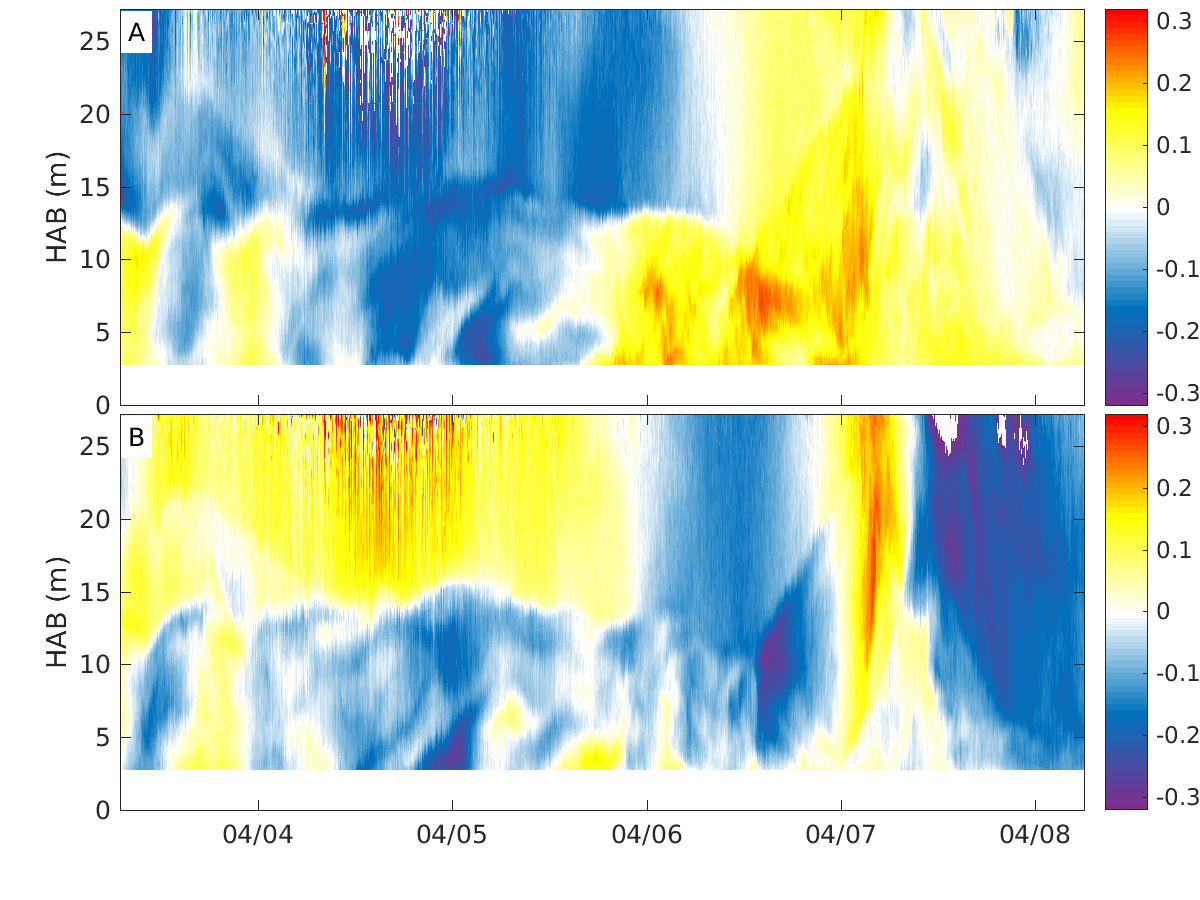
\includegraphics[width=40pc]{bilder/adcp600.png}
 \caption{Time series of velocity profiles obtained with the 600~kHz ADCP on 
Lander 2 during the deployment at TW on cruise AL434 (April 2014).}
 \label{adcp600}
 \end{figure}

\subsection{Tromper Wiek}

During the 5 day instrument deployment in 2014 (\tab{deployments}), we captured 
a storm event with 7 Bft wind and up to 4 m wave height with a consecutive calm 
period (\fig{tromperwiek}, a). In \fig{tromperwiek}, b the variance of the 
horizontal velocity componentsfiltered for wave periods between 2 and 20 
seconds, which is proportional to the kinetic energy contained in the 
waves, is displayed. Although wave energy was maximal in the afternoon of April 
4, the peak in turbidity was not reached until late morning of April, 5. This 
yields that local resuspension during storm did not occur, but a turbid 
watermass was advected to the measurement site. Near bottom current 
(\fig{tromperwiek},C) was directed to the south during the relevant period, i.e. 
water from deeper parts was advected up the slope.
 \begin{figure}[ht]
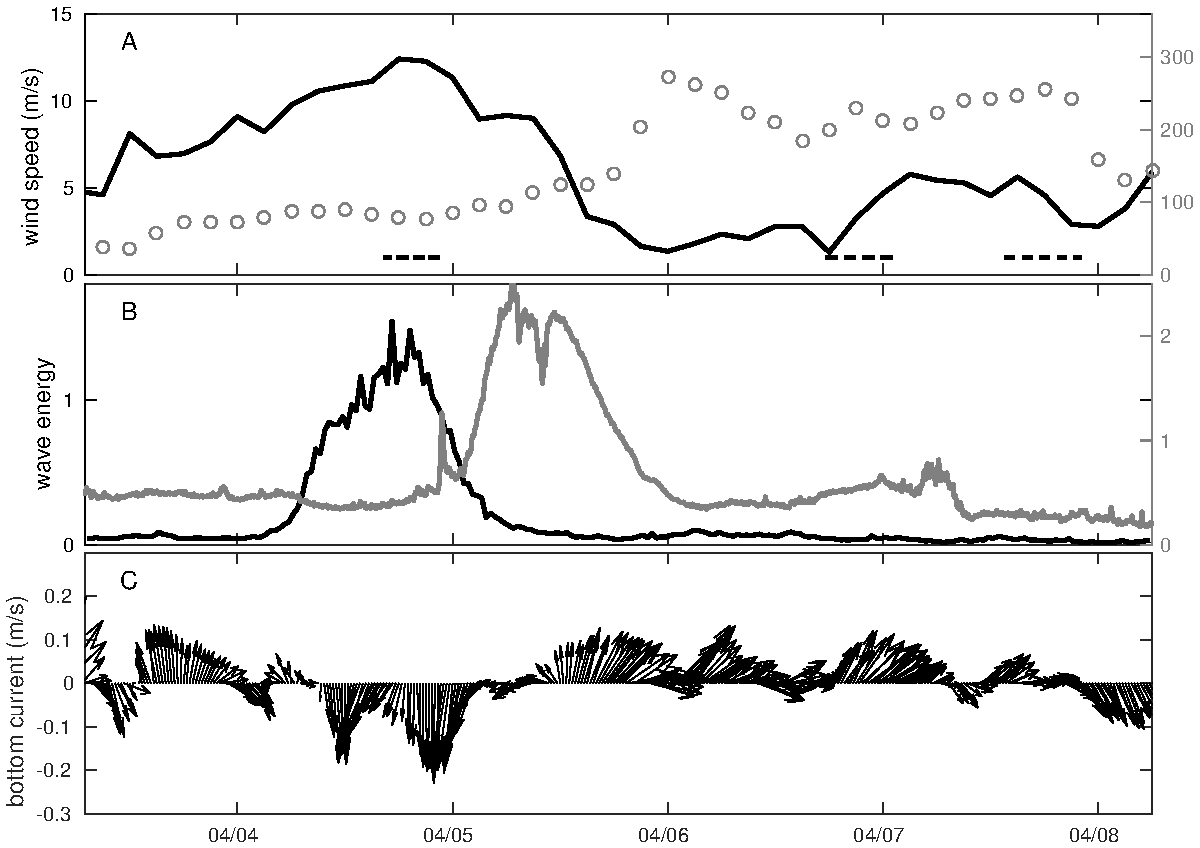
\includegraphics[width=15cm]{bilder/al434tw.pdf}
 \caption{(A) Wind speed and direction from the hindcast of the German Weather 
Service, (B) wave energy and turbidity and (C) direction of 
near bottom current, all obtained with Lander 1 during the deployment at TW on 
cruise AL434 (April 2014).}
 \label{tromperwiek}
 \end{figure}

In the CTD Chain data in \fig{ctdchain} we see a steady increase of the 
near-bottom salinity, accompanied by increasing turbidity. The increase in 
turbidity is clearly linked to the increase of salinity, supporting that turbid 
water is advected to TW from deeper regions below the halocline.

 \begin{figure}[ht]
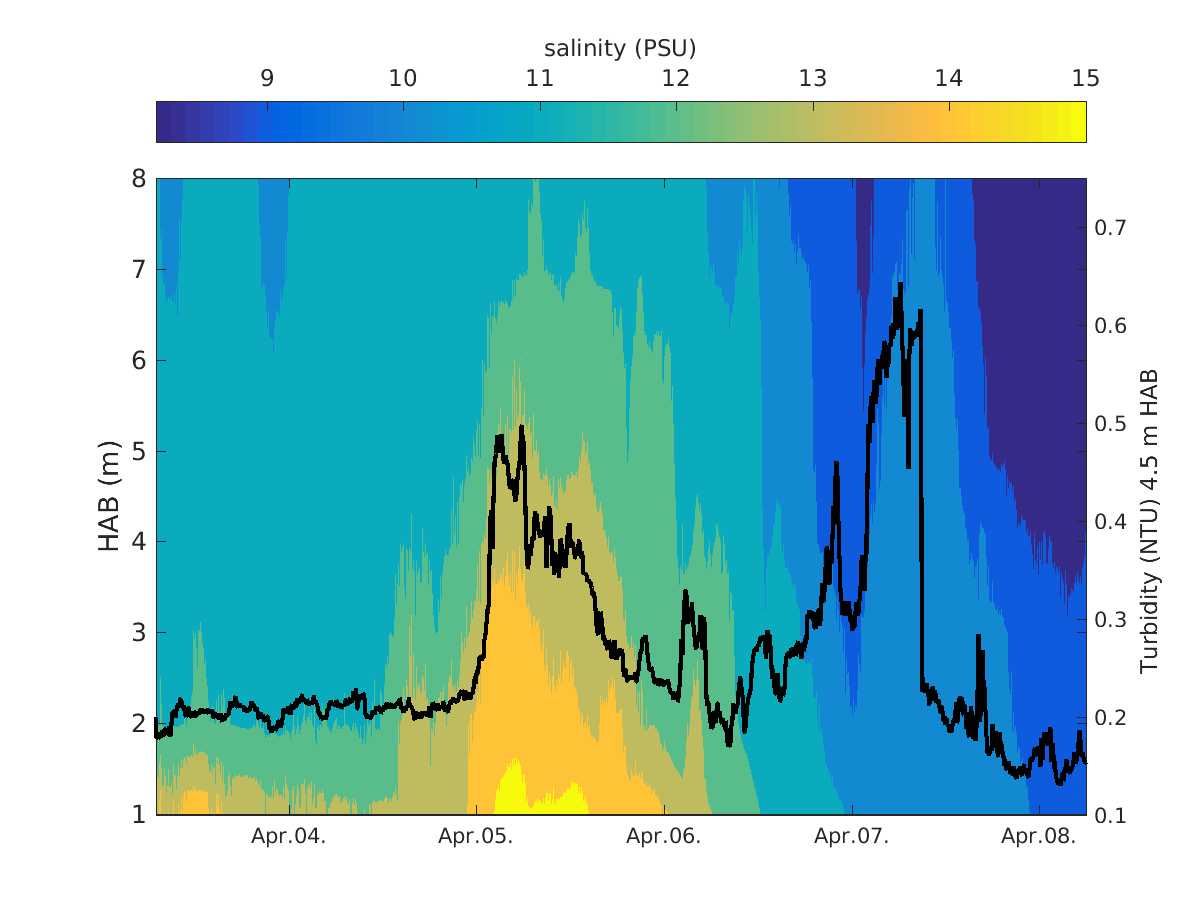
\includegraphics[width=15cm]{bilder/ctdchaintw.png}
 \caption{Salinity (PSU) obtained from the CTD Chain deployed at Tromper Wiek 
during cruise AL434.}
 \label{ctdchain}
 \end{figure}

 This advection of saline water near the bottom is triggered by the local wind 
forcing. Strong easterly wind causes Ekman transport to the north in the 
surface layer \citep[][]{lass2001}, which is visible in the velocity data from 
the 600~kHz ADCP mounted on Lander~2. After the wind decayed, 

\subsection{Transect}

In \fig{transect} we see how the water body is structured along the slope from 
the coast into the basin. A sharp halocline seperates a turbulent bottom 
boundary layer (BBL) of approximately 5 m from the interior. At the left hand 
side of the pannel, where the slope angle steepens, the halocline is widened. 
The boundary layer is generally turbid: Turbidity is more patchy at the upper 
parts of the slope, but high values are confined to the bottom boundary layer, 
so no suspended matter is mixed across the halocline. This indicates that 
turbidity is caused by material originating from the seafloor and held in 
suspension by turbulent motions in the BBL.
Salinity isolines are rather parallel to the slope than straight horizontal, 
what would be the stably stratified case.
  \begin{figure}[ht]
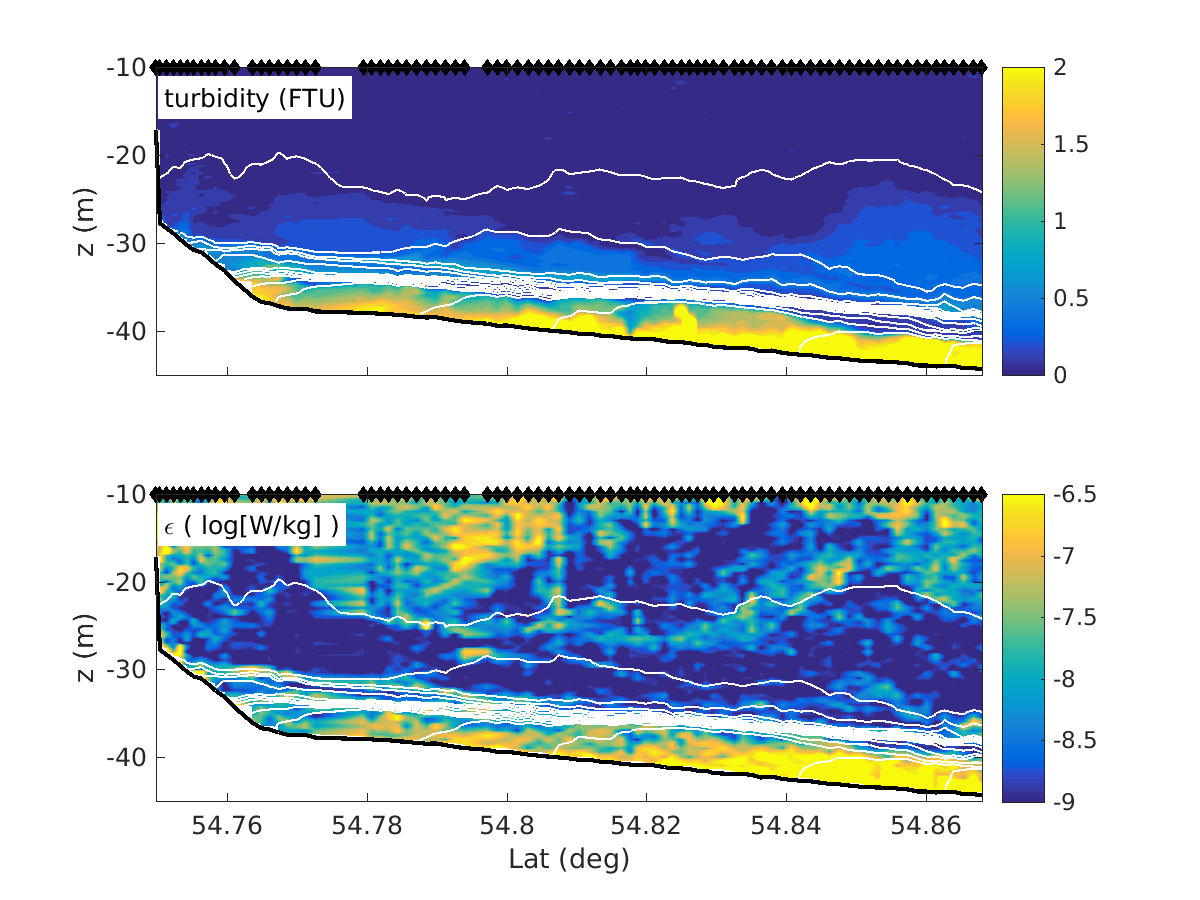
\includegraphics[width=40pc]{bilder/abtrans.png}
 \caption{Turbidity and dissipation rate from the microstructure transect T1. 
White lines indicate levels of equal salinity.}
 \label{transect}
 \end{figure}


\subsection{Arkona Basin}

During each of the three cruises, we collected microstructure data in the 
Arkona Basin. \fig{abmss} shows the profiles of dissipation rate and turbidity, 
averaged over all profiles obtained in the basin for each cruise. A turbulent 
BBL is visible in all three profiles, ranging from 1 to 5 m thickness. 
Turbidity is again enhanced in the BBL, but not above, supporting the data 
described in the last section. As this data set was obtained over three years 
and in different seasons, it is most likely that this turbid, very sharply 
defined BBL is constantly present in the Arkona Basin.
   \begin{figure}[ht]
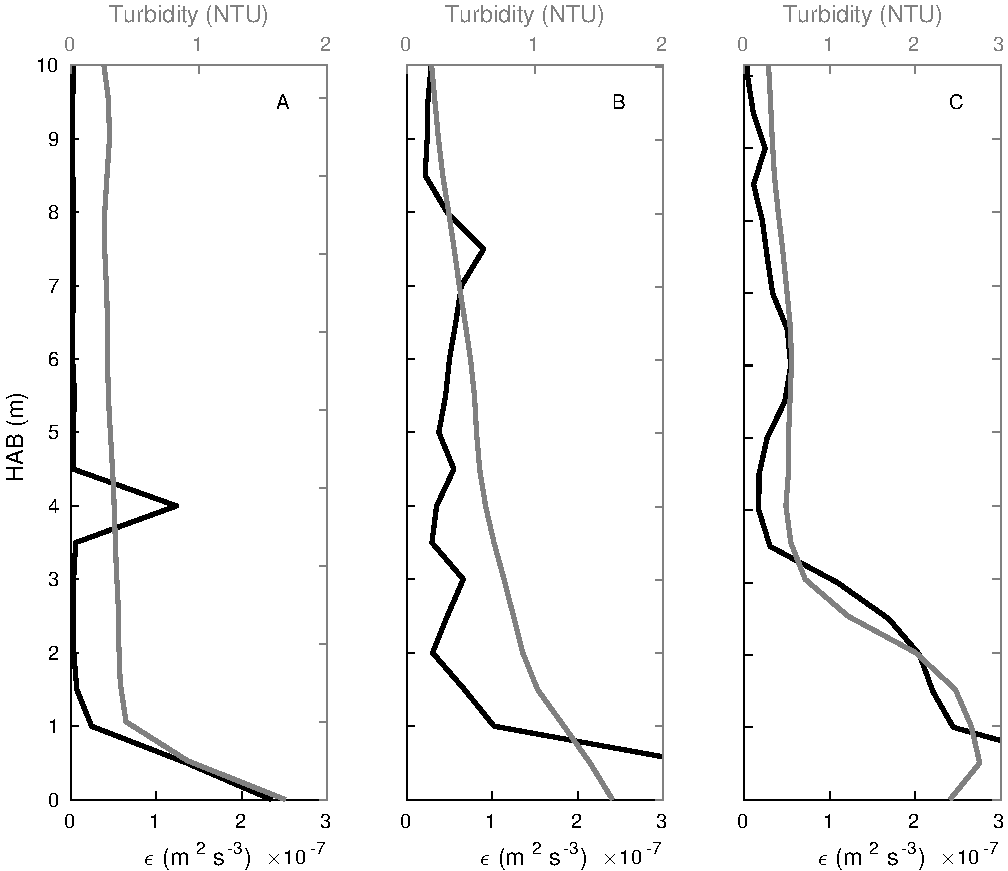
\includegraphics[width=15cm]{bilder/arkona_mss.pdf}
 \caption{Turbidity and dissipation rate from all microstructure transect in 
the Arkona Basin. Solid lines are mean values, dashed line the standard 
deviation. Only the lowermost part of the watercolumn is displayed here.}
 \label{abmss}
 \end{figure}
 
\section{Discussion}

\section{Conclusions}
\chapter{The Effect of Wind Waves on Sediment Properties}
\label{kap-waves}

Wind generated waves are a main contributor to the energetics in shallow water 
bodies. They generate surface mixed layers and influence the near bed dynamics 
even at considerable water depths. In shallow areas, wave induced maximal 
bottom stress mainly dominates over current induced turbulence 
\citep[][]{jonsson2004}. Consequently, waves play a major role in sediment 
transport and distribution in the Baltic Sea.

\section{Introduction}

DEFINITION PERMEABILITY. Sediments that are considered as permeable allow pore 
water flow and exchange by hydrodynamically imposed pressure differences. 
Biogeochemical processes in the sediment are strongly affected by this process, 
and potentially permeable sediments are present in estimately 70$\%$ of the 
global shelf seas. CITE EMERY1968

Permeability is related to grain size distribution and size and geometry of the 
interstices in the sediment. 



\section{Permeability Map}

\cite{forster2003} constructed a map reflecting the permeability in the western 
Baltic Sea using direct measurements of vertical permeability and estimates 
from grain size distribution and porosity. From 37 samples, hydraulic 
conductivity was measured and converted to permeability. From the same samples, 
grain size distribution was determined. An approximation for the permeability 
is the relation of Krumbein and Monk \citep[][]{krumbein1942}
\begin{equation}
 \label{kKM}
 k_{KM} = 7.5 \times 10^{-4} d_{50}^2 e^{-1.31 \sigma},
\end{equation}
where $d_{50}$ is the median diameter and $\sigma$ the standard deviation of 
the grain size distribution. This relation only holds for sufficiently well 
sorted sediments with $\sigma \leq 0.7$. This formula was found to overestimate 
the permeability, thus Eq.\ref{kKM} was divided by a correction factor of 2.6.  
With this new relation, permeability was estimated from two data sets of grain 
size distribution and interpolated. The data are shown in Fig.\ref{perm}.
\begin{figure}[ht]
 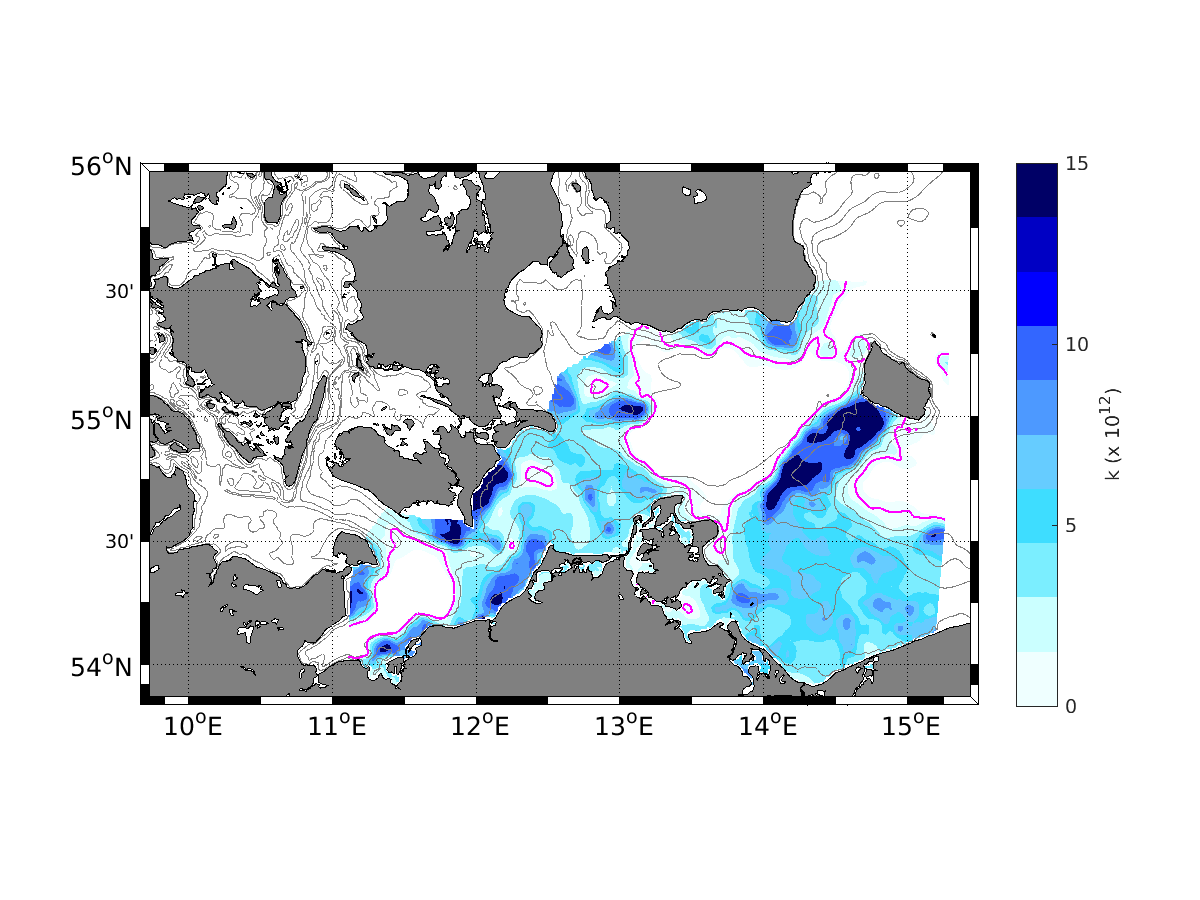
\includegraphics[width=16cm]{bilder/perm_k.png}
 \caption{Permeability data from \cite{forster2003}. Reprinted 
with permission. Pink line indicates the k=$2.5\times10^{-12}$ 
isoline.\label{perm}}
\end{figure}

\section{Wave model for the Baltic Sea}\label{balticswan}

The SWAN wave model version 41.01 was set up for the Baltic Sea including a 
nesting in the area of the German coastal sea. For the whole Baltic Sea, a grid 
resolution of $0.5^\circ \times 0.1^\circ $ in Latitude and Longitude was chosen 
in a domain reaching from $53.5^\circ \text{N } 9^\circ \text{E}$ to $66^\circ 
\text{N } 31^\circ \text{E}$. This includes the Kattegat, the passage from the 
Baltic to the North Sea, where boundary conditions were prescribed in the east: 
A constant JONSWAP spectrum with a wave height of $1$ m, a period of $5$ s and 
peak wave direction of $90^\circ$ with a high directional spreading. The passage 
from the North to the Baltic sea is very shallow, so the boundary conditions 
have negligible influence on the model outcome. Wave frequency range was set to 
0.1 to 1.8 Hz, which mirrors the actual wave frequencies in the Baltic 
Sea \citep[][]{balticsea}, with a resolution of $42$ frequency bins. 
Computations included a spin-up time of $10$ days, sufficient for wave modeling 
and were performed for the years 2013 and 2014. The model was forced by wind 
data from the German Weather Service (DWD), the computational time step was $1$ 
hour (note that the propagation scheme implemented in SWAN is implicit, so the 
time step is not restricted by numerical issues). 

The nesting area reached from $53.5^\circ \text{N } 10^\circ \text{E}$ to 
$55.5^\circ \text{N } 15^\circ \text{E}$, including the Western German coastal 
seas. Spatial resolution was $0.01^\circ \times 0.025^\circ $ in Latitude and 
Longitude and the computational time step was set to $15$ minutes. Boundary 
conditions came from the Baltic Sea model and all parameters were left 
unchanged.

In \fig{verify} the significant wave height calculated with the wave model was 
compared to data obtained with a wave rider buoy. The significant wave height 
is defined as the average wave height of the highest one-third of the waves. 
This value matches the visually observed wave height best and can be calculated 
from the zeroth-order moment if the variance density spectrum $m_0$ via 
$H_{sign} = 4 \sqrt{m_0}$.
\begin{figure}[ht]
 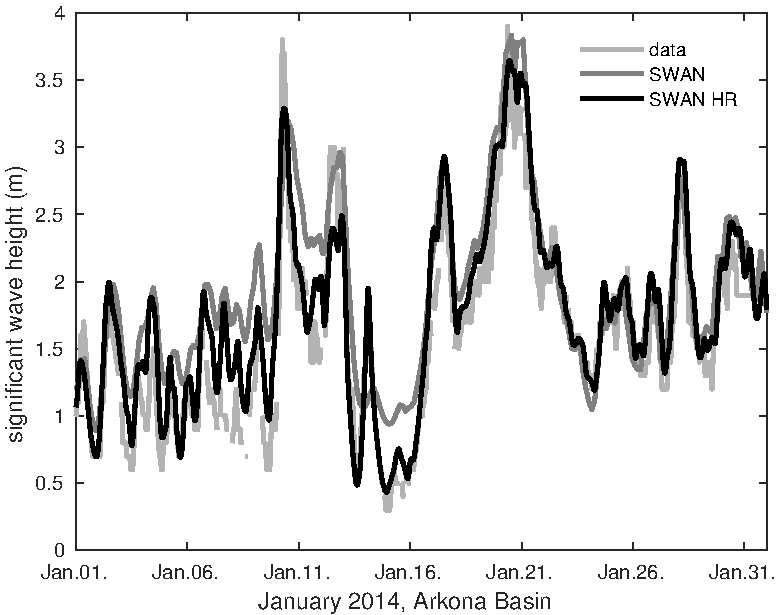
\includegraphics[width=9cm]{bilder/januar.pdf}
 \caption{Significant wave height calculated with the SWAN wave model (HR 
refers to the high resolved nested run) and measured wave height from the 
Arkona wave rider buoy.\label{verify}}
\end{figure}

In the context of a Master Thesis \citep[][]{masterarbeitronja}, the model 
setup for 2013 (still using the previous version SWAN 40.91AB) was 
extensively tested for numerical convergence and compared to measured data on 
several locations in the Baltic Sea. Wave parameters like significant wave 
height were in good agreement with obtained data, even in areas with complex 
topography. A brief description of wind wave properties and processes and a 
discussion the wave model SWAN can be found in Appendix B.

\subsection{Idealized Wind Situations}

Storm surges in the Baltic sea are caused by two large-scale wheater 
situations. Strong northwest or northeast winds generate the highest 
waves in the western Baltic \citep[][]{balticsea}. Northeast winds maximize the 
fetch and therefore the wave activity in German coastal waters. Strong 
northwesterly winds occur more frequently, but tend to last shorter. 

To model wave activity under the two scenarios described above, we forced the 
Baltic Sea wave model with constant wind from the northwest (NW) and the 
northeast (NE), respectively. Wind speed was set to 20 m~s$^{-1}$, which was 
the maximal wind speed reached during a strong northwest wind in January 2005.
We used the same resolution and configuration as described in 
section \ref{balticswan} and a the modeled time period sufficiently long to 
reach stationarity (10 days).

\section{Results}	

\section{Discussion}

\section{Conclusions}
\end{mainmatter}

% Anhaenge -- auskommentieren falls nicht ben\"{o}tigt.
\begin{appendices}
\chapter{Numerical boundary conditions for SPM concentrations}
\pagenumbering{roman}

In view of the strong near-bottom gradients of suspended material, the
implementation of the boundary conditions for the SPM transport
equation \eq{c} requires special attention. While \eq{defFz} provides
an exact expression for the upward turbulent flux $F_z$ at the bottom,
the numerical implementation of the sinking flux,
\begin{equation}
 \label{Fs}
 F_s(z=0) = w_s c_0 \comma
\end{equation}
is not straightforward because the bottom concentration, $c_0$, is
unknown. In vertically staggered numerical grids typically used in
ocean modeling, the bottom concentration $c_0$ has to be estimated
from the known concentration $c_1$ in the center of the lowermost grid
cell, which requires some assumptions about the vertical distribution
of the suspended material in the near-bottom region. While it is
reasonable to assume that the bottom cell is well mixed (i.e.,
$c_0=c_1$) if the bed stress $|\tau_b|$ is smaller than the critical
stress for erosion, $\tau_c$, it is likely that the bottom
concentration $c_0$ is significantly larger than $c_1$ if active
erosion takes place ($|\tau_b| > \tau_c$). In this case, the popular
assumption $c_0=c_1$ may lead to large numerical errors, and to a grid
dependence of the numerical solution. In the following, we show how a
more consistent lower boundary condition can be derived.

We start from the observation that close to the bottom, the transport
equation in \eq{c} reduces to a balance between upward mixing and
downward sinking of suspended material,
\begin{equation}
 \label{cstationary}
 0 = \nu_t^b \partder{c}{z} + w_s c
 \comma
\end{equation}
assuming small slopes ($\alpha \ll 1$) for simplicity. The turbulent
viscosity in the near-bottom region is known to follow the
law-of-the-wall relation $\nu_t = \kappa u_\ast (z + z_0)$, where
$\kappa \approx 0.4$ is the von K{\'a}rm{\'a}n constant, and $u_\ast =
|\tau_b|^{1/2}$ the bottom friction velocity
\citep[e.g.,][]{Pope2000a}. The turbulent diffusivity $\nu_t^b$ in this
region is proportional to $\nu_t$, and therefore adopts the form
$\nu_t^b = Pr_t^{-1} \kappa u_\ast (z + z_0)$, where the turbulent
Prandtl number, $Pr_t$, plays the role of a constant proportionality
factor of order 1. The turbulence model used in our study has been shown to
exactly reproduce this near-wall behavior for $\nu_t$ and $\nu_t^b$
\citep[e.g., ][]{UmlaufBurchard2003a,UmlaufBurchard2005a}.

Inserting the above law-of-the-wall relation for $\nu_t^b$ into
\eq{cstationary}, we find a solution of the form
\begin{equation}
 \label{Rouse}
 \dfrac{c}{c_0} = \left( \frac{z}{z_0} + 1 \right)^{-p} \comma
\end{equation}
which is recognized as the classical Rouse profile
\citep{vanRijn84b}, slightly modified here by the appearance of the
turbulent Prandtl number in the definition of the Rouse number $p =
w_sPr_t \, / (\kappa u_\ast)$.

Recalling that in any conservative numerical scheme, $c_1$ represents
the average concentration inside the lowermost grid cell, a relation
between $c_0$ and $c_1$ may be found from integrating \eq{Rouse}
across the cell. If we denote $h$ as the cell thickness, this yields
\begin{equation}
 \label{cbot}
 c_0 = \frac{c_1}{r} \quad \text{for} \quad |\tau_b|>\tau_c \comma
\end{equation}
where 
\begin{equation}
 \label{rr}
 r =  \frac{1}{(1-p) h/z_0} \left[ \left( \frac{h}{z_0} + 1 \right)^{1-p} -1 \right] 
 \comma
\end{equation}
\begin{figure}[ht]
  \noindent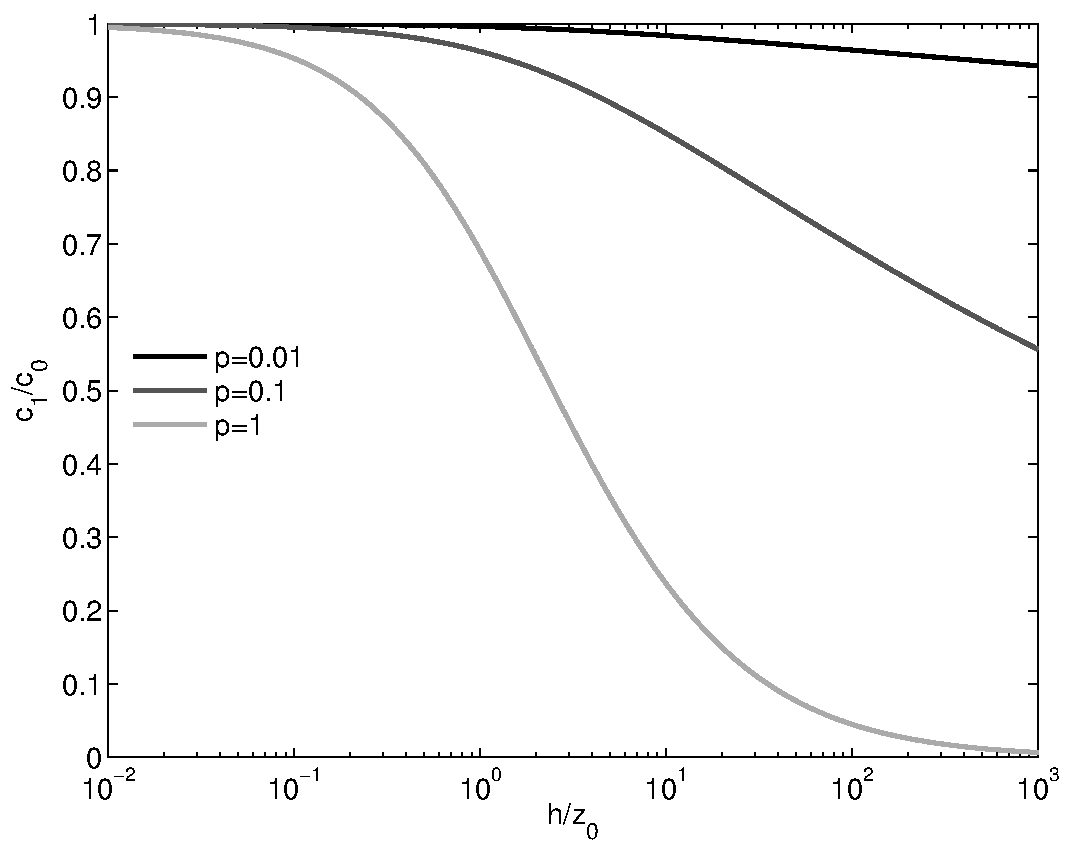
\includegraphics[width=29pc,angle=0]{bilder/rouse.pdf}\\
  \caption{A1}{Concentration ratio $c_1/c_0$ as a function of
    non-dimensional cell thickness, $h/z_0$, for different Rouse
    numbers according to \eq{cbot}.\label{c0c1}}
\end{figure}
Fig. A1 shows the ratio $r=c_1/c_0$ as a function of the normalized
cell thickness $h/z_0$ for different Rouse numbers. The most important
conclusion from this figure is that the naive approach of assuming
$c_0 = c_1$ to compute the sinking flux in \eq{Fs} during erosion
periods introduces large numerical errors except for small Rouse
numbers and/or extremely fine grids with $h \ll z_0$. Below, we
nevertheless discuss some reference solutions that satisfy this
condition. We note, however, that the constraint $h \ll z_0$ implies
$\Delta t \ll z_0 / w_s$ for the numerical time step according to the
well-known CFL stability criterion for explicit advection schemes. It
is easy to show that, even for idealized one-dimensional simulations,
the numerical effort may become prohibitively large for small $z_0$.

Using the example from Section \ref{sec:bbl} above, Fig. A2
illustrates that assuming $c_0 = c_1$ during both erosive and
non-erosive periods leads to significant numerical errors, and to a
grid-dependence of the results. 
\begin{figure}[ht]
  \noindent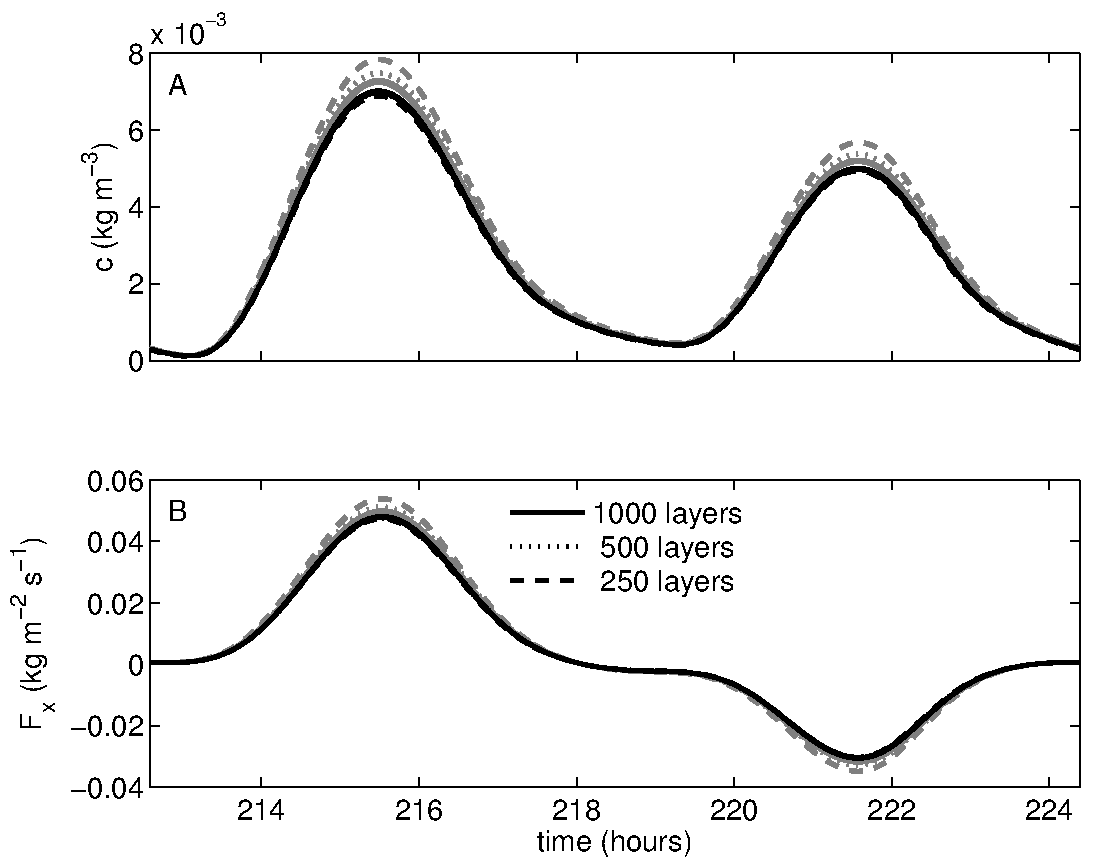
\includegraphics[width=29pc,angle=0]{bilder/appendix.pdf}\\ \caption{A2}{Numerical
    results for (a) SPM concentration 5~m above the bottom, and (b)
    upslope flux $F_x$ for three vertical resolutions. Gray lines are
    based on the assumption $c_0 = c_1$ to compute the sinking flux in
    \eq{Fs}, whereas black lines are based on \eq{cbot} during erosive
    periods. Parameters correspond to Case 1 in
    \tab{params}. \label{convergence}}
\end{figure}
Estimating $c_0$ based on \eq{cbot}
during periods with active erosion, however, removes this dependency
on the numerical grid, and leads to stable results already for
moderate vertical resolution. All results discussed in this manuscript
are therefore based on this new expression. Convergence studies were
carried out to insure that all our results are independent of the
numerical grid size and time step.
\chapter{State of the art wind wave modeling}

In this appendix, supplementary information about wind wave generation and 
evolution is given, followed by a discussion of the third generation wave model 
SWAN, including the latest findings to improve the theory.

\section{Evolution of Waves}

The spectrum of vertical motions of the ocean surface consists of several types 
of waves, covering a broad frequency range.  Wind generated 
waves have periods around $0.25 - 30\,\text{s}$. Locally generated waves, 
called 
wind sea, are irregular and short crested. While propagating away from the 
generation area, they become long crested and more regular, their periods 
increase. These waves are called swell \citep[][]{holthuijsen2007}. 

\subsection{Wave Generation by Wind}
Energy is transferred from wind to the waves by wind-induced surface pressure 
fluctuations. 
Under the assumption of a harmonic wave propagating in the same direction as 
the (faster) wind 
blows, the wind field near the water surface is disturbed as indicated in 
\fig{windgen}. Higher air pressure is induced at the windward site of the wave 
crest, where the water surface moves downwards while the wave is propagating, 
and vice versa low air pressure at the leeward site of the wave crest, where 
the sea surface is moving upwards.
\begin{figure}[ht]

 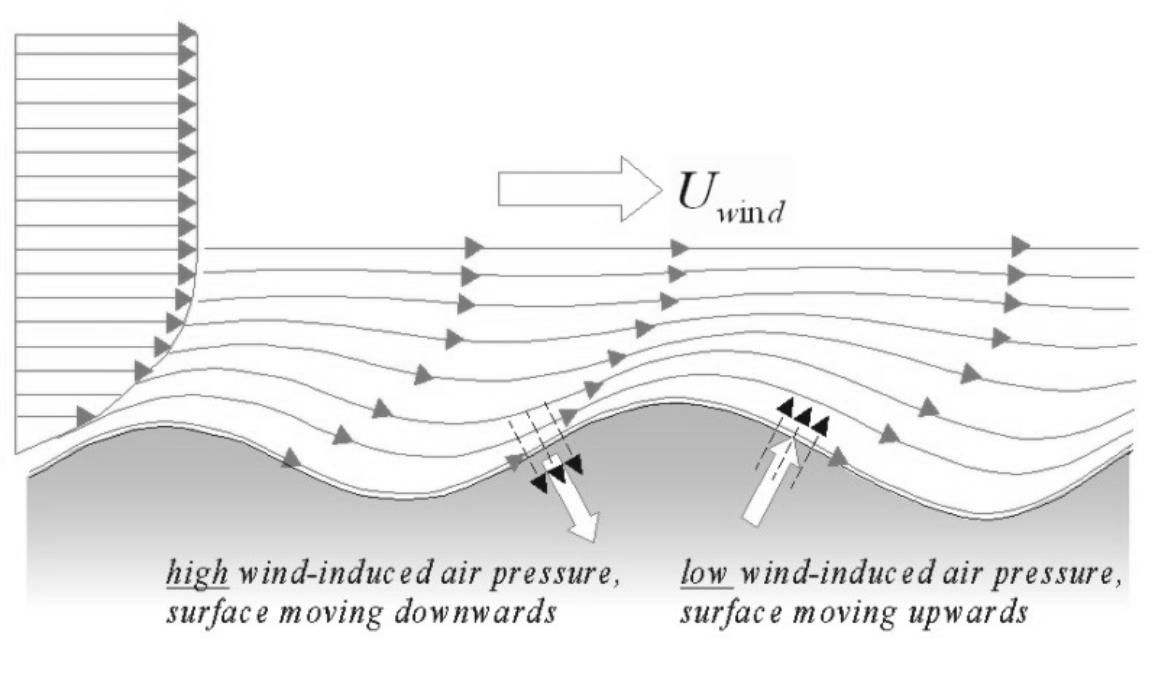
\includegraphics[width=10cm]{bilder/windpressure_sw.png}
 \caption{Wind-pressure distortions over a propagating harmonic wave. Figure 
taken from \cite{holthuijsen2007}. \label{windgen}}
\end{figure}

This way, the (wave-induced) air pressure distortions amplify the vertical 
movement of the water surface, transfering energy from wind to the wave field. 
This process enforces itself as it is more effective for higher waves. Wave 
growth ends when the wave propagation speed approaches wind speed. It is not 
well understood how initial distortions of the sea surface are generated, but 
fortunately wave growth is not sensitive to the initial wave field.

\subsubsection{Wave Growth Limitation}

Wave growth (in deep water) is not only limited by the wind speed 
$U_{10}$, as mentioned above, but also by the time that wind has been blowing 
and the distance to the coast where the wind comes from. This distance is 
called fetch, and wave height increases the longer the fetch is. Wind duration 
and fetch can be combined to the equivalent fetch, assuming that from the 
moment on that the wind started, a wave component with group velocity $c_g$ has 
travelled a certain distance in wind direction. Wind transfers the same 
energy to the wave component either over a time $t$ or (for an infinitely long 
time period) over a distance
\begin{equation}
 \label{eqFetch}
 F_{eq} = c_g t \cos \theta , 
\end{equation}
where $\theta$ is the wave propagation direction relative to the wind 
direction. This distance is called the equivalent fetch. Sea states where real 
fetch is shorter (longer) than the equivalent one are called fetch-limited 
(duration-limited). At fully developed sea states, the wave phase speed (at 
some peak frequency) has approached $U_{10}$ and wave growth decays.

\subsection{Wave-wave Interaction}

Energy can be transfered between wave components by resonance. This happens, if 
two pairs of waves have the same frequency, wave number vector and direction. A 
pair of waves is a superposition of two waves of different frequencies and wave 
number vectors, which visually form a diamond pattern (\fig{diamond}).
\begin{figure}[ht]
 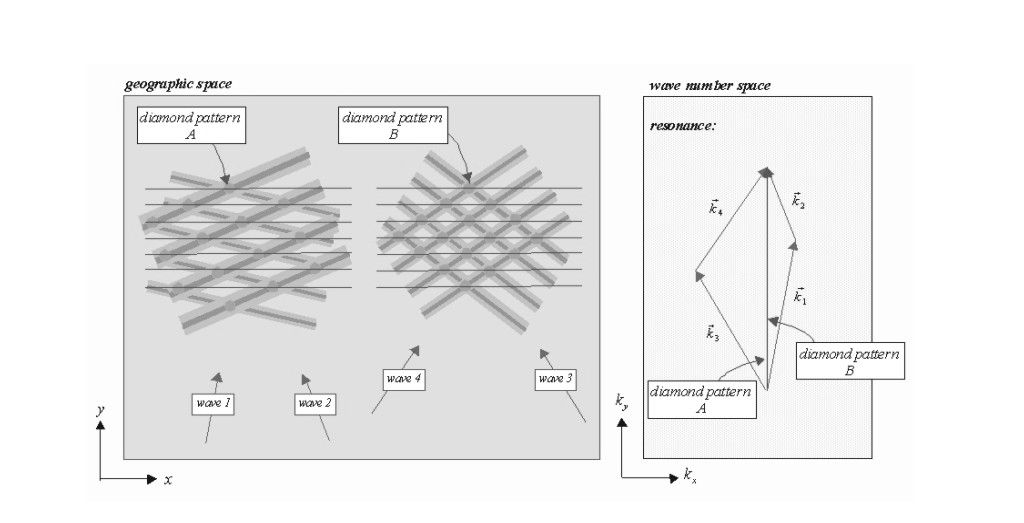
\includegraphics[width=15cm]{bilder/diamond.png}
 \caption{Two pairs of waves, each creating a diamond pattern, fulfill the 
resonance conditions fow quadruplet wave-wave interaction. Figure taken from 
\cite{holthuijsen2007}. \label{diamond}}
\end{figure}

If two of those diamond patterns fulfill the resonance conditions, energy can 
be distributed among the four waves involved. This mechanism is called 
quadruplet wave- wave interaction. It draws energy from the mid-range 
frequencies and provides it to waves with rather high or low frequencies. 

In shallow water (non-dispersive waves), triad wave-wave interaction is 
possible, where a pair of waves fulfills the above resonance conditions with a 
third wave. In deep water, the required resonance conditions cannot be 
fulfilled because of the dispersion relationship.

\subsection{Dissipation of Energy}

Wave energy can be dissipated either by white-capping in deep 
water, or by bottom friction and depth-induced breaking in the surf zone. 

White-capping describes the breaking of waves in deep water. This is a 
highly non-linear process which is not understood in detail. Presumably, wave 
steepness and local wind affect the occurrence of white-caps, which draw energy 
from waves at frequencies by hindering the upward movement of the sea surface. 
The dissipative effect of white-capping is rather weak.

\section{Sea State Description}
The most important method 
to describe a sea state is to treat ocean waves as a stochastic process to 
calculate a wave spectrum, from which parameters like wave height are derived. 
One possibility therefore is the random-phase/amplitude model, described in 
detail in \cite{holthuijsen2007}: The time series of surface elevation $ \eta 
(t)$ is assumed to be a superposition of $N$ sinusoidal waves, each with a 
distinct frequency $f_i$, amplitude $a_i$ and phase $\alpha_i$, written as
\begin{equation}
 \label{sinussum}
 \eta(t) = \sum_{i=1}^N a_i \cos (2\pi f_i t + \alpha_i).
\end{equation}
Considering $a_i$ and $\alpha_i$ to be independent random variables, 
probability density functions for both can be derived from observations. For 
waves in sufficiently deep water which are not too steep, it was found that the 
phase is uniformly distributed (and can therefore be omitted in the wave 
spectrum), while the amplitude is Rayleigh distributed with expected value 
$E\{a_i\} = \mu_i$ for each frequency $f_i$. The function $f_i \rightarrow 
E\{a_i\}$ is called the amplitude spectrum and already contains all 
(non-directional) information of the sea state. A more meaningful 
characterization is, however, the variance spectrum $f_i \rightarrow E\{a_i^2 
\slash 2\}$, as the variance is proportional to the wave energy contained in 
each frequency, with the proportionality constant $\rho g$. Here, $\rho$ 
denotes 
density of the water and $g$ the gravitational acceleration. By scaling the 
variance of each discrete frequency with the frequency bin $\Delta f$ (i.e. the 
size of the frequency resolution) and formally assuming infinitely small 
frequency bins, the variance density spectrum is obtained. Multiplied by the 
factor $\rho g$, this is the energy density spectrum:
\begin{equation}
 \label{vardensspec}
 E(f) = \rho g \lim_{\Delta f \rightarrow 0} \frac{1}{\Delta f} E\{\frac{1}{2} 
a_i^2\}.
\end{equation}
For a harmonic wave, i.e. all wave energy is contained in one distinct 
frequency, $E(f)$ reduces to a delta distribution. For more irregular waves, 
the 
energy density spectrum broadens. 

The shape of this spectrum is not at all arbitrary, but was found to have 
rather uniform characteristics under similar conditions. For a fully 
developed sea state, the Pierson-Moskowitz (PM) spectrum was derived: 
\begin{equation}
 \label{PMspectrum}
 E_{PM}(f) = \underbrace{\alpha_{PM}g^2(2 
\pi)^{-4}f^{-5}}_{f^{-5}\text{-tail}} \underbrace{\exp \left[ - \frac{5}{4} 
\left( \frac{f}{f_{PM}} \right)^{-4} \right]}_{\text{low-freq. cut-off}}.
\end{equation}
The $f^{-5}$ - tail comes from a dimensional argument under the assumption, 
that wave breaking limits the spectra on the high frequency side, and that this 
process is determined only by the gravitational acceleration and the wave 
frequency itself. Therefore, $E(f) \sim g^2f^{-5}$ at high frequencies. At a 
peak frequency $f_{PM}$, depending on the wind speed, a smooth low-frequency 
cut-off is imposed. From observations, an energy scale of $\alpha_{PM} = 
0.0081$ was derived.

The PM spectrum describes a fully developed sea state, i.e. 
constant wind conditions being present until sea state becomes stationary and 
no fetch limitation is assumed. Observed sea states rarely fulfill these 
assumptions, and during an extensive study, the JONSWAP (Joint North Sea wave 
Project, \cite{hasselmann1974}) spectrum for young sea states was designed:
\begin{equation}
 \label{JONSWAPspectrum}
 E_{JONSWAP}(f) = \underbrace{\alpha g^2(2 
\pi)^{-4}f^{-5} \exp \left[ - \frac{5}{4} \left( \frac{f}{f_{\text{peak}}} 
\right)^{-4} \right]}_{\text{PM shape}} \underbrace{\gamma^{\exp \left[ - 
\frac{1}{2} \left( \frac{f}{\sigma f_{\text{peak}}} \right)^2 \right]}}_{G(f)}.
\end{equation}
Here, the PM spectrum was down-scaled with a higher peak frequency 
$f_\text{peak}$ and a smaller energy scale $\alpha$ (which depends on the 
$f_\text{peak}$ now) to maintain the shape of the PM spectrum. $G(f)$ is a peak 
enhancement function, which amplifies and narrows the spectrum around the peak 
frequency. Hereby, $\gamma$ and $\sigma$ control height and width of the peak, 
respectively. 

The JONSWAP spectrum was found to be a good generalization of observed wave 
energy spectra, not only for idealized fetch-limited conditions but also for 
arbitrary wind conditions. Reason for that is that wave-wave interaction (see 
above) distributes energy among wave frequencies in a way that stabilizes the 
shape of the JONSWAP spectrum. 

The energy spectra discussed above are one dimensional, only depending on wave 
frequency. No information about the propagation direction of waves are 
included. To completely describe a sea state, the energy spectrum $E(f,\theta)$ 
has to be extended by informations about how energy is distributed among waves 
traveling in propagation direction $\theta$.

\section{Third Generation Wave Model SWAN}

The open source wave model SWAN, an acronym for \textbf{S}imulating 
\textbf{WA}ves \textbf{N}earshore, is a wave model optimized for applications in 
coastal waters. As the spatial resolution of model domains in coastal regions is 
often very fine to capture smaller features in topography, SWAN has an implicit 
propagation scheme implemented, assuring numerical stability even for timesteps, 
that violate the CFL criterion. 

The central equation that is solved for every timestep at every grid point is 
the action balance equation, that accounts not only for the energy 
distributions 
in the wave frequency space but also for frequency shifts by wave-current 
interaction. The action density $N=N(\sigma,\theta; x,y,t)$ is therefore 
dependent on the relative radian frequency $\sigma$, which is the shifted 
frequency in a system moving with the current: 
\begin{equation}\label{ebe}
 \frac{\partial N}{\partial t} + \frac{\partial c_{g,x} N}{\partial x} + \frac{ 
\partial c_{g,y} N}{\partial y} + \frac{\partial c_{\theta} N}{\partial \theta} 
+ 
\frac{\partial c_{\sigma} N}{\partial \sigma}= \frac{S_{in} + S_{nl} + 
S_{wc}}{\sigma},
\end{equation}
where the source terms on the right hand side refers to energy input by wind, 
nonlinear wave -- wave interaction and energy dissipation by white capping. $t, 
x ,y$ are time and spatial directions, $\theta$ is the direction of wave energy 
propagation and $c_{g,x}, c_{g,y}$ are the group speed in each spatial 
direction. The fifth term on the left had side represents the frequency shift 
by 
ambient currents.

In the absence of currents, this action balance equation reduces to the energy 
balance equation.
\begin{equation}\label{ebe}
 \frac{\partial E}{\partial t} + \frac{\partial c_{g,x} E}{\partial x} + \frac{ 
\partial c_{g,y} E}{\partial y} + \frac{\partial c_{\theta} E}{\partial \theta} 
= 
S_{in} + S_{nl} + S_{wc}.
\end{equation}
All equations in the following will be noted, consistent with the action balance 
equation, in terms of the relative radian frequency $\sigma$. Although various 
formulations for the different mechanisms below are implemented in SWAN, only 
the ones used in the setup for the Baltic Sea in chapter \ref{balticswan} are 
described.

\subsection{Wave generation by wind}

Wind data is provided to the model as the wind speed and direction at 10 m 
elevation, $U_{10}$. This value is converted to a friction velocity via
\begin{equation}
 u_\ast^2 = C_D U_{10}^2.
\end{equation}
Before version 41.01 of SWAN, the wind drag coefficient was linearly dependent 
on the wind speed with an imposed lower limit. This formulation was found to 
overestimate $C_D$ for strong winds. Therefore, \cite{zijlema2012} fitted a 
second-order polynomial to nearly 5000 observed wind drag coefficients in 
dependence of the wind speed and came up with 
\begin{equation}
 C_D = \left( 0.55 + 2.97 \dfrac{U_{10}}{U_{ref}} - 1.49 \left( 
\dfrac{U_{10}}{U_{ref}} \right)^2 \right) \times 10^{-3} ,
\end{equation}
where $U_{ref} = 31.5 \, \text{m s}^{-1}$ is the wind speed at which $C_D$ is 
maximal.

The source term for energy input by wind includes two mechanisms:
\begin{equation}\label{gen}
 S_{in} (f, \theta) = \alpha + \beta E(f,\theta),
\end{equation}
where $\alpha$ is the initial wave growth, parameterized with the following 
empirical expression by Cavaleri and Malanotte--Rizzoli
\begin{equation}
 \alpha = 
 \begin{cases}
  \dfrac{1.5 \cdot 10^{-3}}{g^2 2 \pi} \left(u_\ast \cos{(\theta - 
\theta_{wind})}\right)^4 G & \text{for } |\theta - \theta_{wind}| \le 90^\circ  
\\
  0 & \text{for } |\theta - \theta_{wind}| \textgreater 90^\circ  \\
 \end{cases}
\end{equation}
where $G$ is a cut-off function to avoid wave growth at frequencies below the 
Pierson--Moskowitz frequency, $g$ the gravitational acceleration and 
$\theta_{wind}$ is the wind direction. 

Another implemented approach to quantify the initial wave growth is to impose 
the JONSWAP spectrum for young sea states. The non-dimensional peak wave 
frequency $\tilde{f}_{peak} = f_{peak} U_{10} / g$ is thereby derived using the 
spatial step size at each point as fetch $F$ with an empirical equation by 
\cite{kahma1992} for short fetch lengths:
\begin{equation}
 \tilde{f}_{peak} = 2.18 \tilde{F}^{-0.27},
\end{equation}
where $\tilde{F} = g F / U_{10}^2$. All other coefficients in the JONSWAP energy 
spectrum equation are derived from this peak frequency 
\citep[][]{holthuijsen2007}, and  wave directions are assumed to be $\cos^2$ 
distributed.

For the exponential wave growth term $\beta$ in \eqref{gen} the classical 
expression of \citep[][]{komen1984} is used:
\begin{equation}
 \beta = \max \{ 0,0.25 \frac{\rho_{air}}{\rho_{water}} \left[28 
\frac{u_\ast}{c} \cos(\theta - \theta_{wind}) -1 \right] \} \sigma,
\end{equation}
with the phase velocity $c$ and $\rho_{air}$ and $\rho_{water}$ the densities of 
air and water.

\subsection{Nonlinear wave -- wave interaction}

The calculation of quadruplet wave-wave interaction requires large 
computational resources because of the high number of possible quadruplet 
constellations. It is calculated with the discrete-interaction approximation 
(DIA) by \citep[][]{hasselmann1985}. Only two constellations of wave 
quadruplets 
are considered to interact. The frequencies must fulfill
\begin{align*}
 \sigma_1 &= \sigma_2 = \sigma \\
 \sigma_3 &= 1.25 \sigma = \sigma^+ \\
 \sigma_4 &= 0.75 \sigma = \sigma^- .\\
\end{align*}
The wave directions must be equal for the waves with frequency $\sigma$, while 
the waves with frequencies $\sigma_3$ and $\sigma_4$ lie at angles of $\theta_1 
= -11.5^\circ \; \left[ \text{or } \theta_1 = 11.5^\circ \right]$ and $\theta_2 
= 33.6^\circ \; \left[ \text{or } \theta_2 = -33.6^\circ \right]$  to them. The 
contribution for each quadruplet to the source term $S_{nl}$ in Eq. (\ref{ebe}) 
is:
\begin{equation}
 S_{nl4}^\ast (\sigma, \theta) = 2 \delta S_{nl4} (\alpha_1 \sigma, \theta) - 
\delta S_{nl4} (\alpha_2 \sigma, \theta) - \delta S_{nl4} (\alpha_3 \sigma, 
\theta),
\end{equation}
where for $i \in \{1,2,3\}$
\begin{align*}
 \delta S_{nl4} ( \alpha_i \sigma, \theta ) = & 2.12 \cdot 10^{(-4)} \sigma^{11} 
\cdot [ ( 0.41 E(\alpha_i \sigma^+, \theta)E^2(\alpha_i \sigma, \theta) \\
 &+ 3.16 E(\alpha_i \sigma^-, \theta) ) - 54.6 E(\alpha_i \sigma, \theta) 
E(\alpha_i \sigma^+, \theta) E^2(\alpha_i \sigma^-, \theta) ] .
\end{align*}
The coefficients are $\alpha_1 = 1, \, \alpha_2 = 1.25, \, \alpha_3 = 0.75$. 

The above holds for infinite water depth and must be multiplied with a scaling 
factor 
\begin{equation}
 R ( \tilde{k}d ) = \max \{ 1+ \frac{22}{3}\tilde{k}d \left( 1-\frac{6}{7} 
\tilde{k}d \right) \times \exp(-1.25 \tilde{k}d) , 4.43 \} ,
\end{equation}
depending on the mean wave number $\tilde{k}$ and the the water depth $d$ to 
obtain the finite depth contribution to the source term for nonlinear wave -- 
wave interaction.

\subsection{Dissipation}

Wave energy is dissipated by white -- capping. The representation of this 
process originates from \citep[][]{hasselmann1974}:
\begin{equation}
 S_{wc} (\sigma, \theta ) = - 2.36 \cdot 10^{-5} \frac{k}{\tilde{k}} \left( 
\frac{\tilde{s}}{\tilde{s}_{PM}} \right)^4 \frac{\tilde{\sigma}}{\tilde{k}} k 
E(\sigma, \theta),
\end{equation}
with $\tilde{s} = \tilde{k} \sqrt{m_0}$ being the overall wave steepness, $k$ 
the wave number, $\tilde{\sigma}$ the mean wave frequency and $\tilde{s}_{PM} = 
\sqrt{3.02 \times 10^{-3}}$ the overall wave steepness of the Pierson -- 
Moskowitz spectrum.
\end{appendices}

\begin{backmatter}
% Verweis auf Literaturverzeichnis zum Inhaltsverzeichnis hinzufuegen
\addtocontents{toc}{\vspace*{1em}}

% Literaturliste aus Literaturdatenbank (Bibtex-Datei) bauen. Nur tatsaechlich zitierte Literatur wird in Liste aufgenommen.
% Regelmaessigen Aufruf von ``bibtex abschlussarbeit'' nicht vergessen, falls das der Latex-Editor nicht
% erledigt.
% Zur Bearbeitung der Literaturdatenbank kann das Programm JabRef (http://jabref.sf.net) empfohlen werden. (Java-Programm, laeuft unter Windows, Linux, Mac, ...)
\bibliography{literatur}
% Stil fuer Literaturliste festlegen
% Variante A: DIN, Eintraege erhalten Kuerzel aus Autoren-Initialien und Jahr, alphabetisch geordnet
% \bibliographystyle{alphadin}
% Variante B: DIN, Eintraege werden durchnummeriert, alphabetisch geordnet
\bibliographystyle{ametsoc2014}


\begin{abstract}[Selbständigkeitserklärung]
\thispagestyle{empty}
Ich versichere hiermit an Eides statt, dass ich die vorliegende Arbeit selbstständig
angefertigt und ohne fremde Hilfe verfasst habe, keine außer den von mir
angegebenen Hilfsmitteln und Quellen dazu verwendet habe und die den benutzten
Werken inhaltlich und wörtlich entnommenen Stellen als solche kenntlich gemacht
habe.
\vspace*{2cm}

\flushright{
Rostock, (\today)
}
\end{abstract}

\end{backmatter}

\end{document}
